%%%%%%%%%%%%%%%%%%%%%%%%%%%%%%%%%%%%%%%%%%%%%%%%%%%%%%%%%%%%%%%%%%%%%%%%%%%%%%%%%%%%%%%%%%%%%%%%%%%%%%%%%%%%%%%
%%%%%%%%%%%%%%%%%%%%%%%%%%%%%%% Fit to real data for tty total measurement %%%%%%%%%%%%%%%%%%%%%%%%%%%%%%%%%%%%
%%%%%%%%%%%%%%%%%%%%%%%%%%%%%%%%%%%%%%%%%%%%%%%%%%%%%%%%%%%%%%%%%%%%%%%%%%%%%%%%%%%%%%%%%%%%%%%%%%%%%%%%%%%%%%%
\subsection{Inclusive \tty Measurement (\tty prod. + \tty dec.):}
\label{sec:tty_total_measurement}
 In this section, we will present results of the unfolded likelihood fit using data for the incusive \tty (\tty prod. + \tty dec.) cross section measurement. After the fit, the resulting post-fit $p_T(\gamma)$ distribution are shown in Figure~\ref{fig:pt_postfit_ljet_tty_total_realdata} for the single lepton channel and in Figure~\ref{fig:pt_postfit_dilep_tty_total_realdata} for the dilepton channel. The resulting pulls of the NPs  are shown in Figure ~\ref{fig:pull_plot_pt_ljet_mu_blinded_tty_total}, Figure ~\ref{fig:pull_plot_pt_dilep_mu_blinded_1_tty_total} and the correlations in Figure ~\ref{fig:NP-corr_ljet_mu_blinded_tty_total} and Figure ~\ref{fig:NP-corr_dilep_mu_blinded_tty_total}, for the lepton+jets and dilepton channels, respectively. The post-fit value of all the NPs changed within 1 $\sigma$, with a large fraction of the NPs having very small pulls and constrains, which indicate that the fit is robust and not affected by any unexpected behavior of the NPs. Ranking plots are shown in Figures ~\ref{fig:ranking_ljet_total_mu_blinded} and ~\ref{fig:ranking_dilep_total_mu_blinded} for single lepton and dilepton channels. The unfolded distributions at particle level are shown in Figures ~\ref{fig:pt_unfolded_ljet_tty_total_realdata} and ~\ref{fig:pt_unfolded_dilep_tty_total_realdata_1} and ~\ref{fig:pt_unfolded_dilep_tty_total_realdata_2} for single lepton and dilepton channels. Furthermore, the Norm Factors are shown in Figures ~\ref{fig:pt_unfolded_ljet_table_tty_total_realdata} and ~\ref{fig:pt_unfolded_dilep_table_tty_total_realdata} for single lepton channel and dilepton channel respectively. The normalized unfolded distributions are shown in Figures ~\ref{fig:tty_total_diff_Ljets_norm} and ~\ref{fig:tty_total_diff_DL1_norm} for single lepton and dilepton channels respectively. The decomposed uncertainties of the unfolded distributions for the absolute differential cross-sections are illustrated in Figures ~\ref{fig:tty_total_diff_Ljets_groupedimpact} and ~\ref{fig:tty_total_diff_DL1_groupedimpact}, ~\ref{fig:tty_total_diff_DL2_groupedimpact} for single lepton channel and dilepton channel respectively. $\chi^2$/ndf and $p$-values between the measured absolute and normalised cross-sections of the total \tty production and decay process and the LO $2\rightarrow 7$ \MGNLO simulation interfaced with \PYTHIA[8] and \HERWIG[7] are shown in Table ~\ref{tab:chi2_tty}.




%The parameter of interests $\mu$ (inclusive \tty. signal strength) are
%blinded throughout the process. This means that the value of 
%this parameter will not be revealed until the end of the 
%analysis, ensuring a fair and unbiased evaluation of the 
%model's performance. The purpose of this approach is to 
%ensure that any potential biases or preconceptions do 
%not influence the interpretation of the results, while checking the behavior of the nuisance 
%parameters in the fit to the data. 


%the NPs are behaving as expected.  
%are robust and not affected by any unexpected behavior of the NPs.

%In summary, by keeping the POIs blinded throughout 
%the process, we have ensured a fair and unbiased 
%evaluation of the model's performance, and by studying 
%the behavior of the NPs, we have validated the 
%robustness of our results.

\begin{figure}[ht]
  \centering
  \subfloat[]{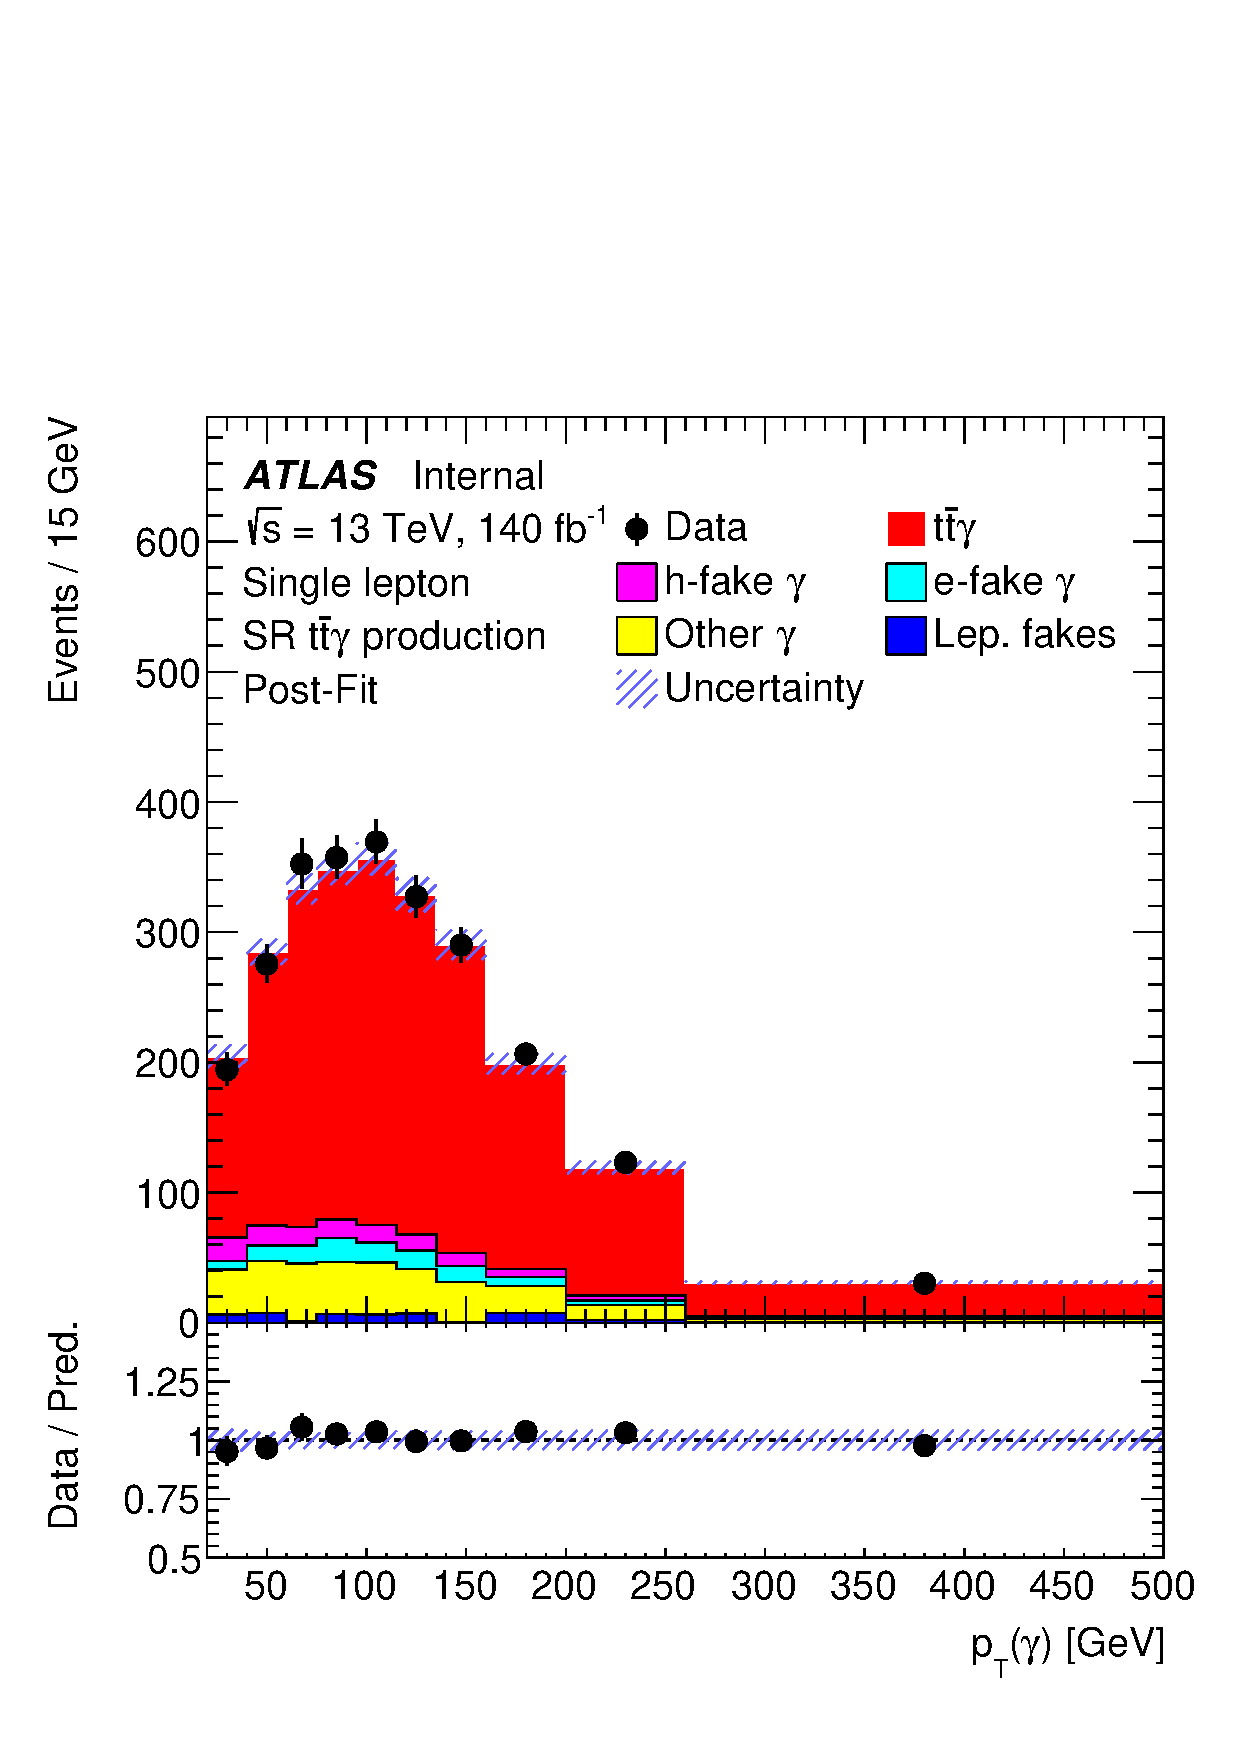
\includegraphics[width=0.30\textwidth]{figures/diff_xsec/ljet_tty_total/post_fit/tty1l_pt_all_syst/Plots/SR1_postFit.pdf}}
  \quad\quad
  \subfloat[]{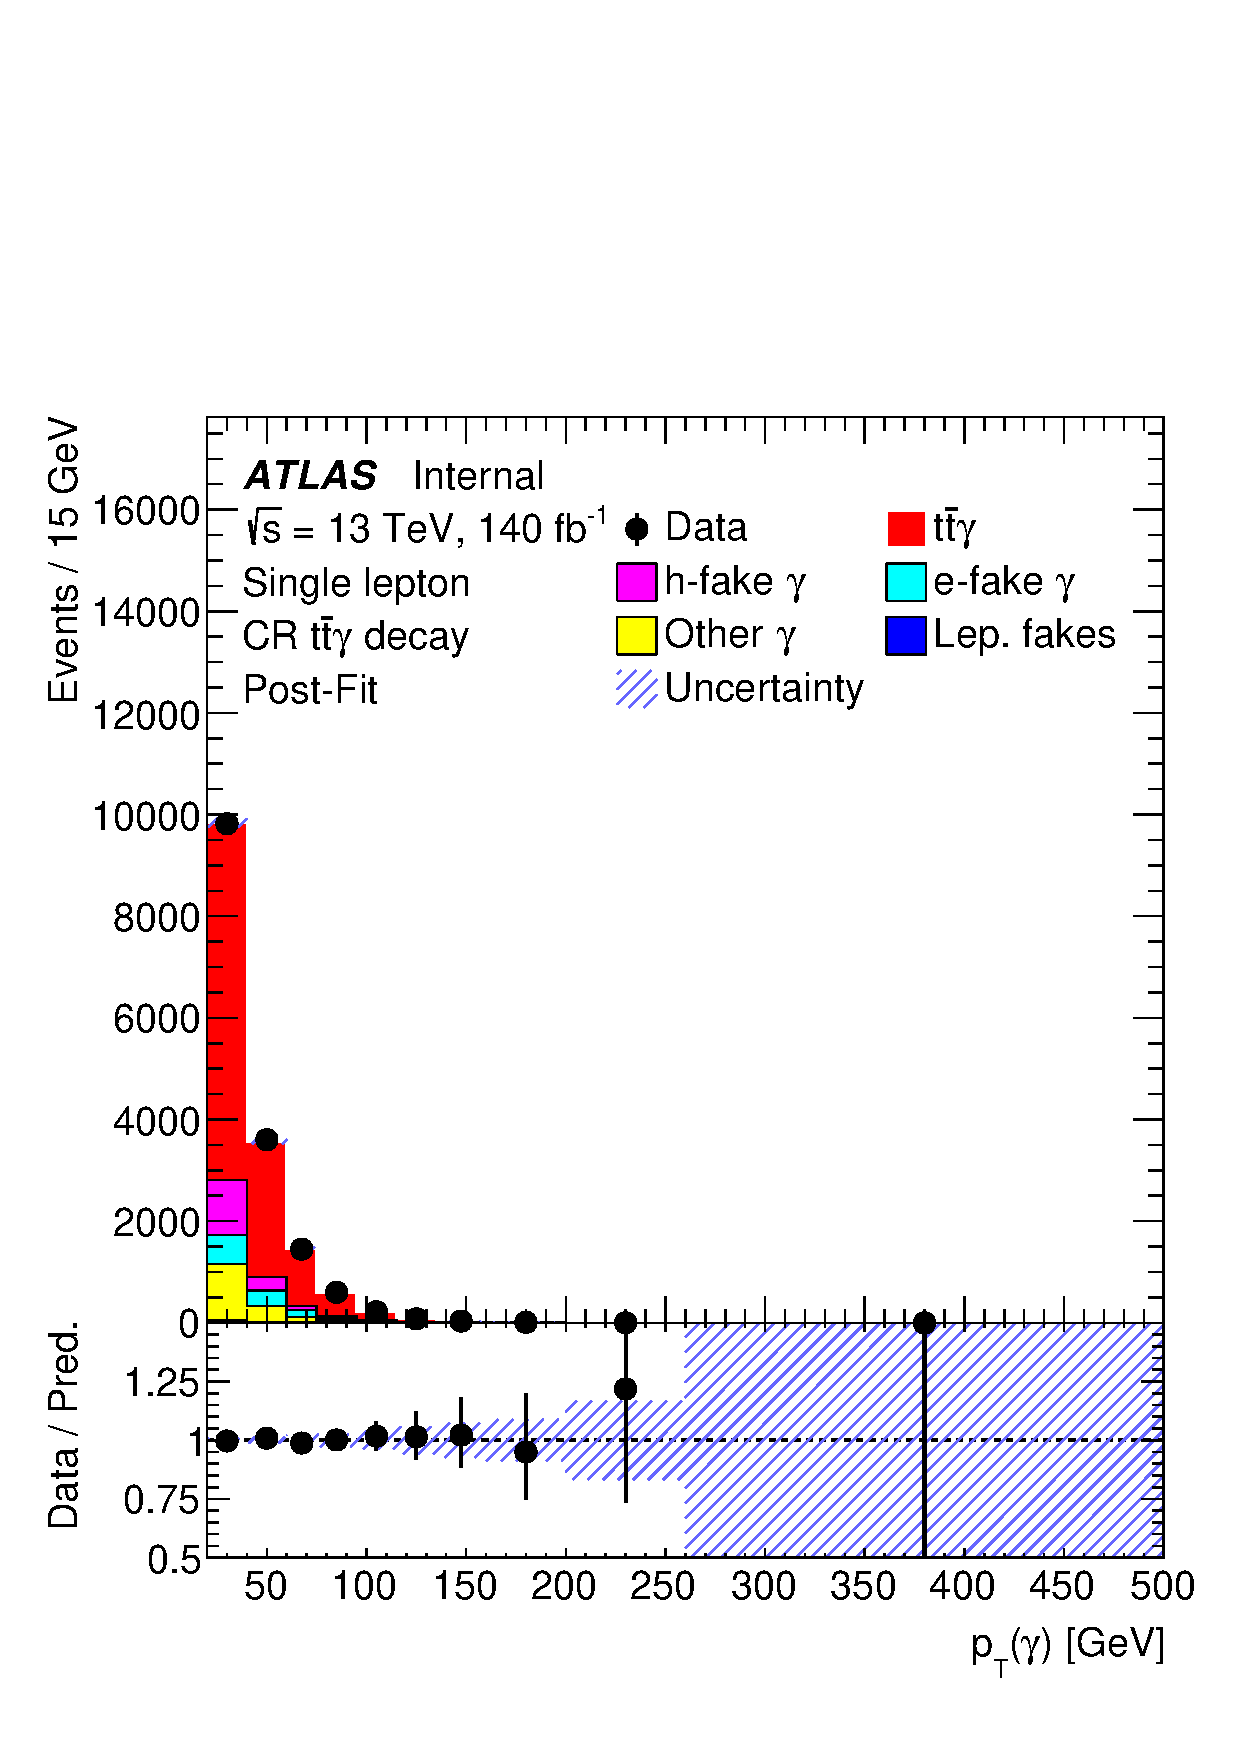
\includegraphics[width=0.30\textwidth]{figures/diff_xsec/ljet_tty_total/post_fit/tty1l_pt_all_syst/Plots/SR2_postFit.pdf}}
  \quad\quad
  \subfloat[]{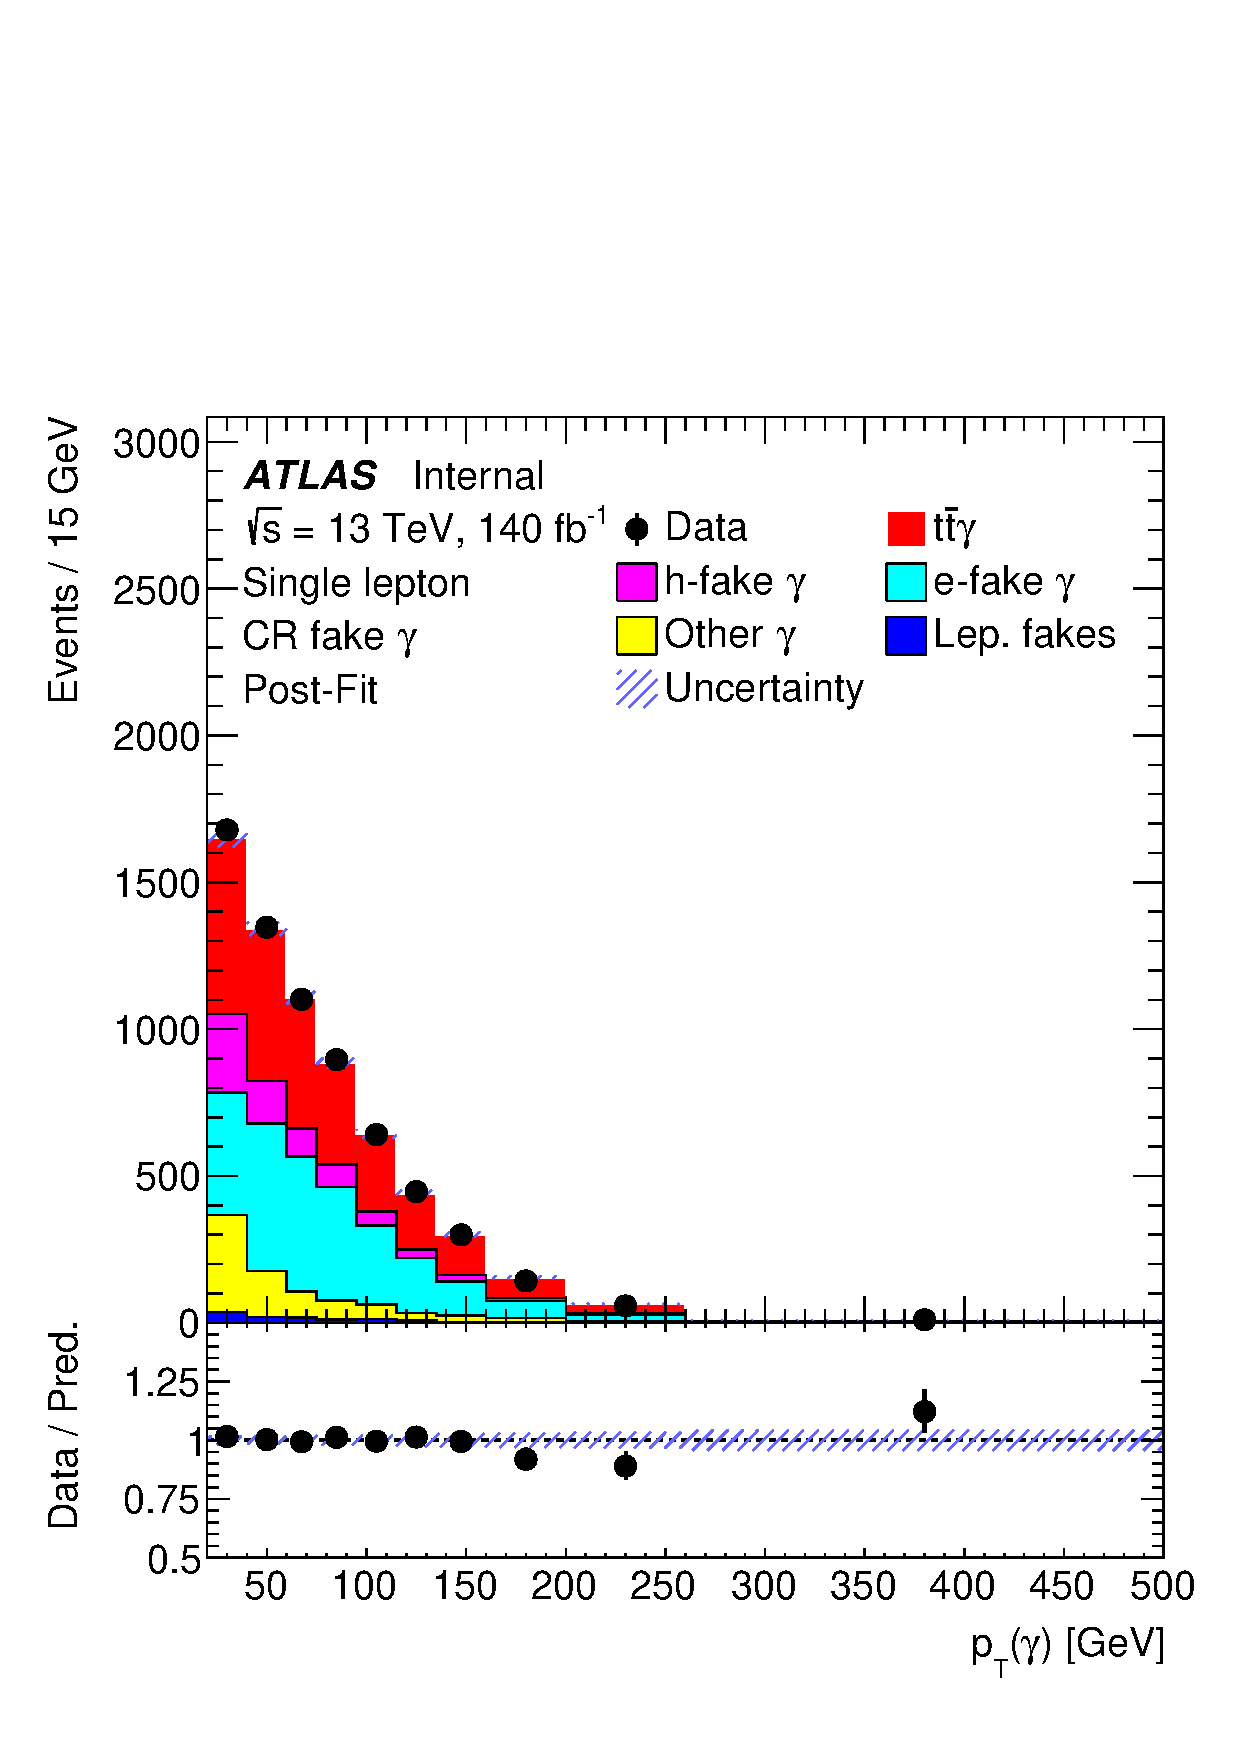
\includegraphics[width=0.30\textwidth]{figures/diff_xsec/ljet_tty_total/post_fit/tty1l_pt_all_syst/Plots/SR3_postFit.pdf}}
  \quad\quad
  \subfloat[]{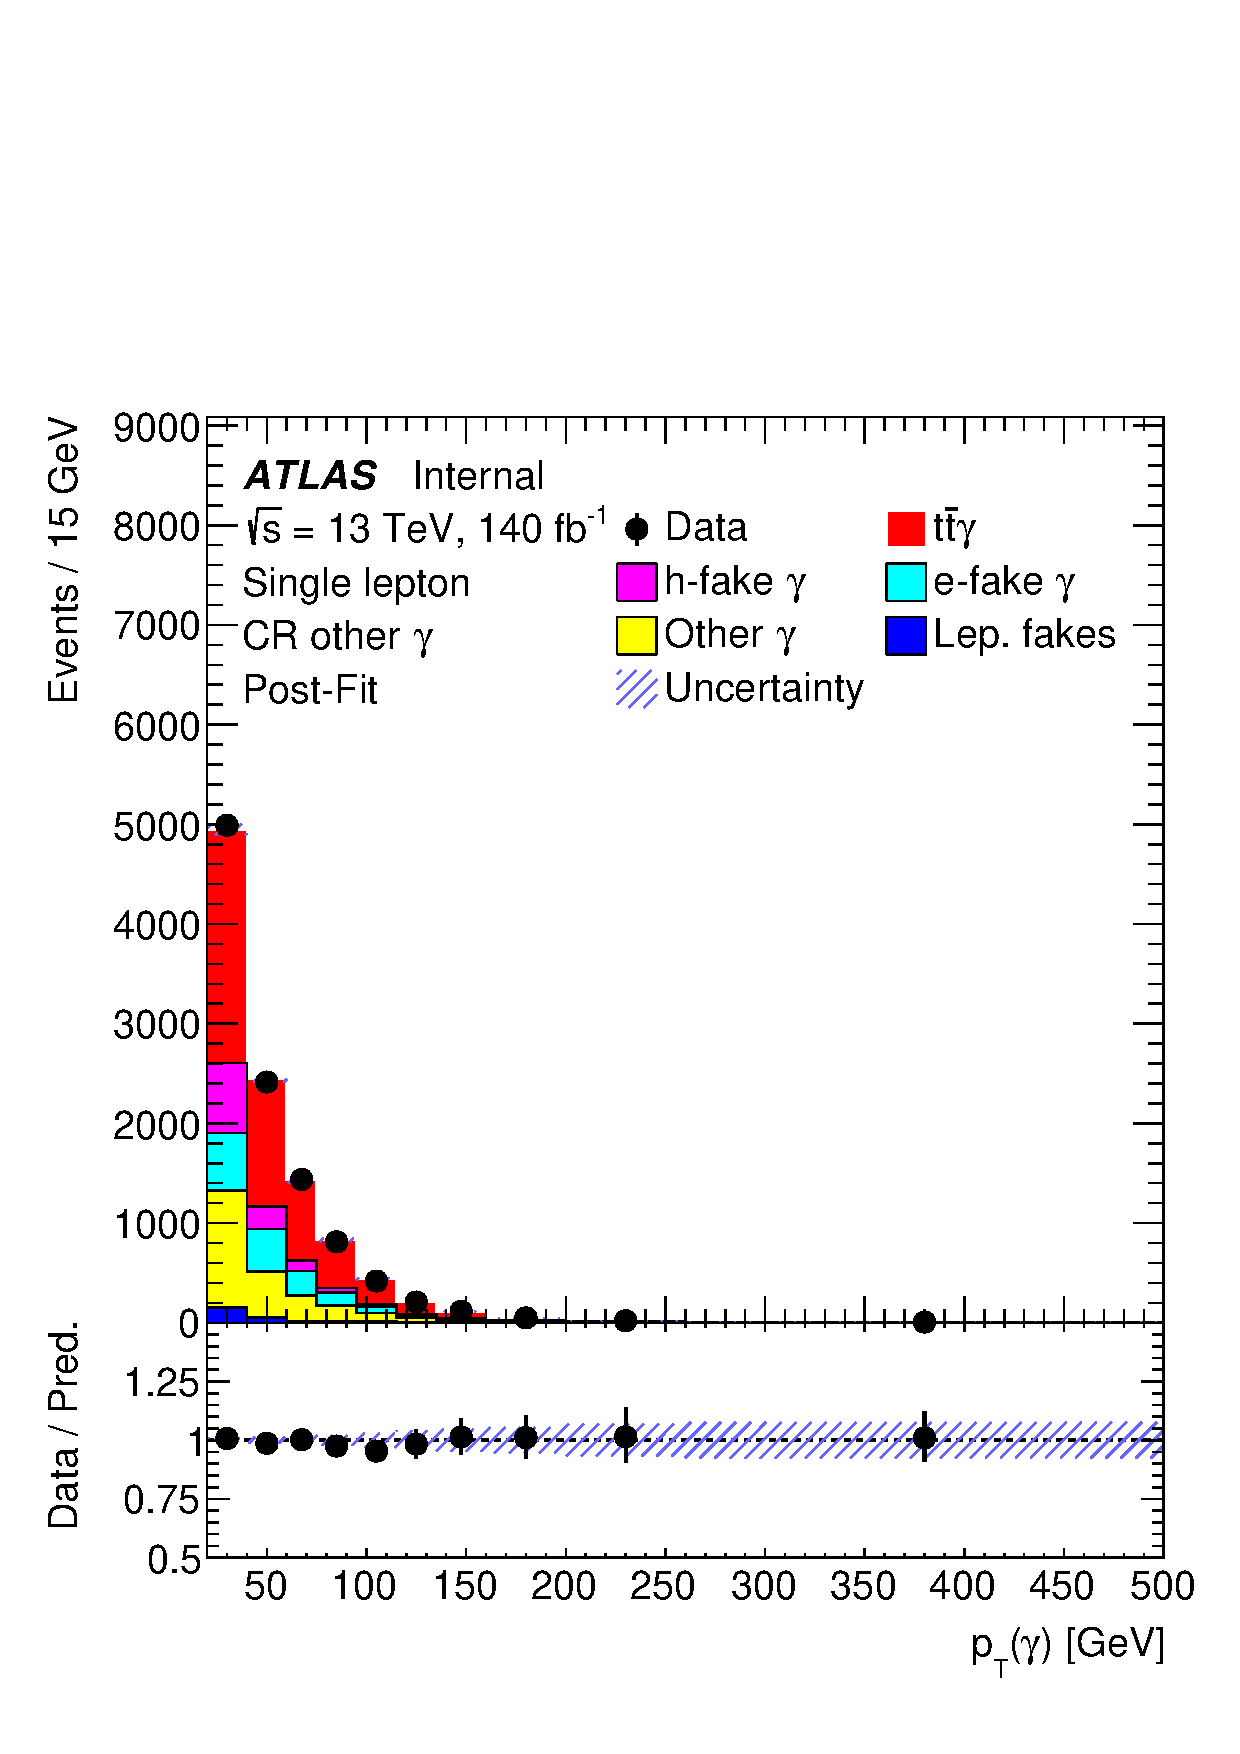
\includegraphics[width=0.30\textwidth]{figures/diff_xsec/ljet_tty_total/post_fit/tty1l_pt_all_syst/Plots/SR4_postFit.pdf}}

  \caption{The post-fit distributions of $p_T(\gamma)$ in 4 regions ( (a) \tty (prod.) enriched region  (b) \tty (dec.) enriched region
  (c) fakes enriched region (d) prompt photon enriched region) in single lepton channel. }
  \label{fig:pt_postfit_ljet_tty_total_realdata}
\end{figure}
\FloatBarrier


\begin{figure}[ht]
  \centering
  \subfloat[]{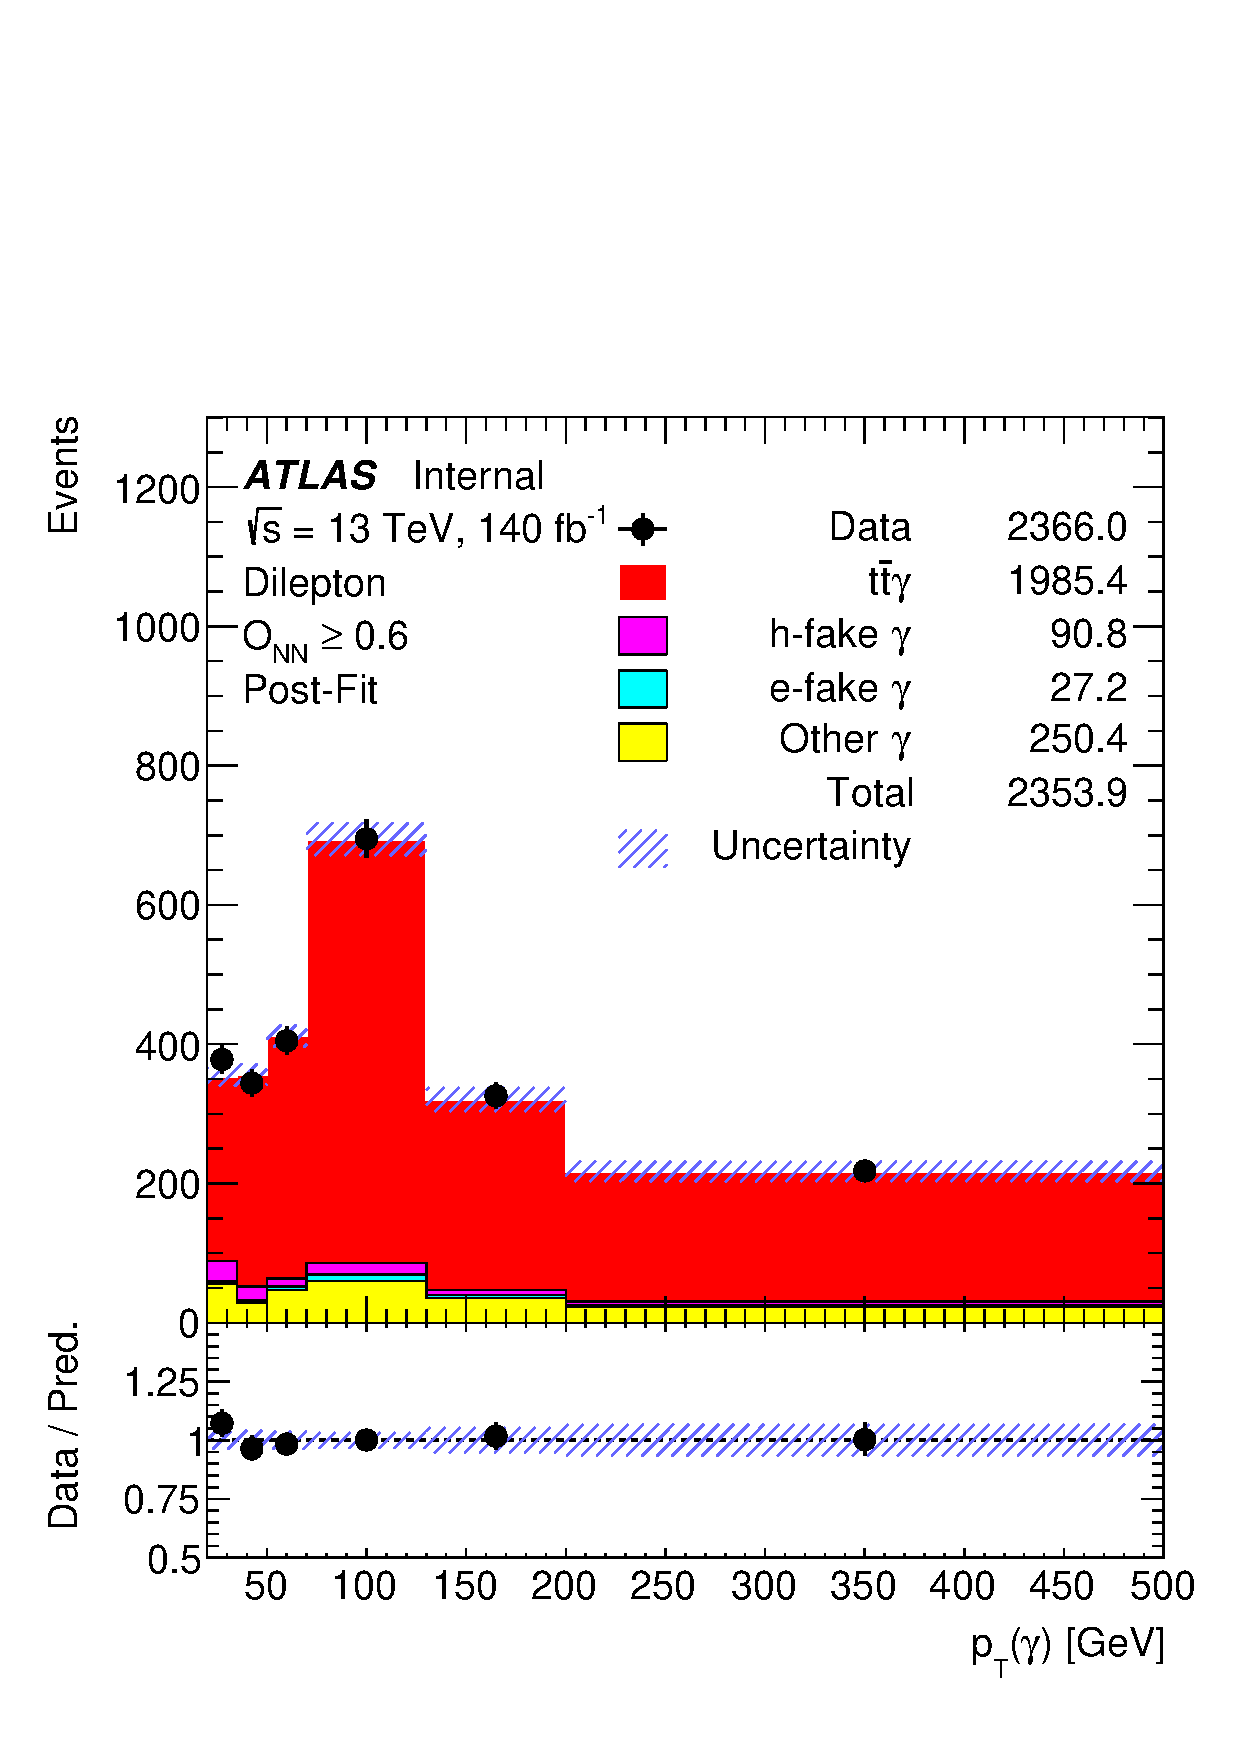
\includegraphics[width=0.30\textwidth]{figures/diff_xsec/dilep_tty_total/post_fit/tty2l_pt_all_syst/Plots/SR1_postFit.pdf}}
  \quad\quad
  \subfloat[]{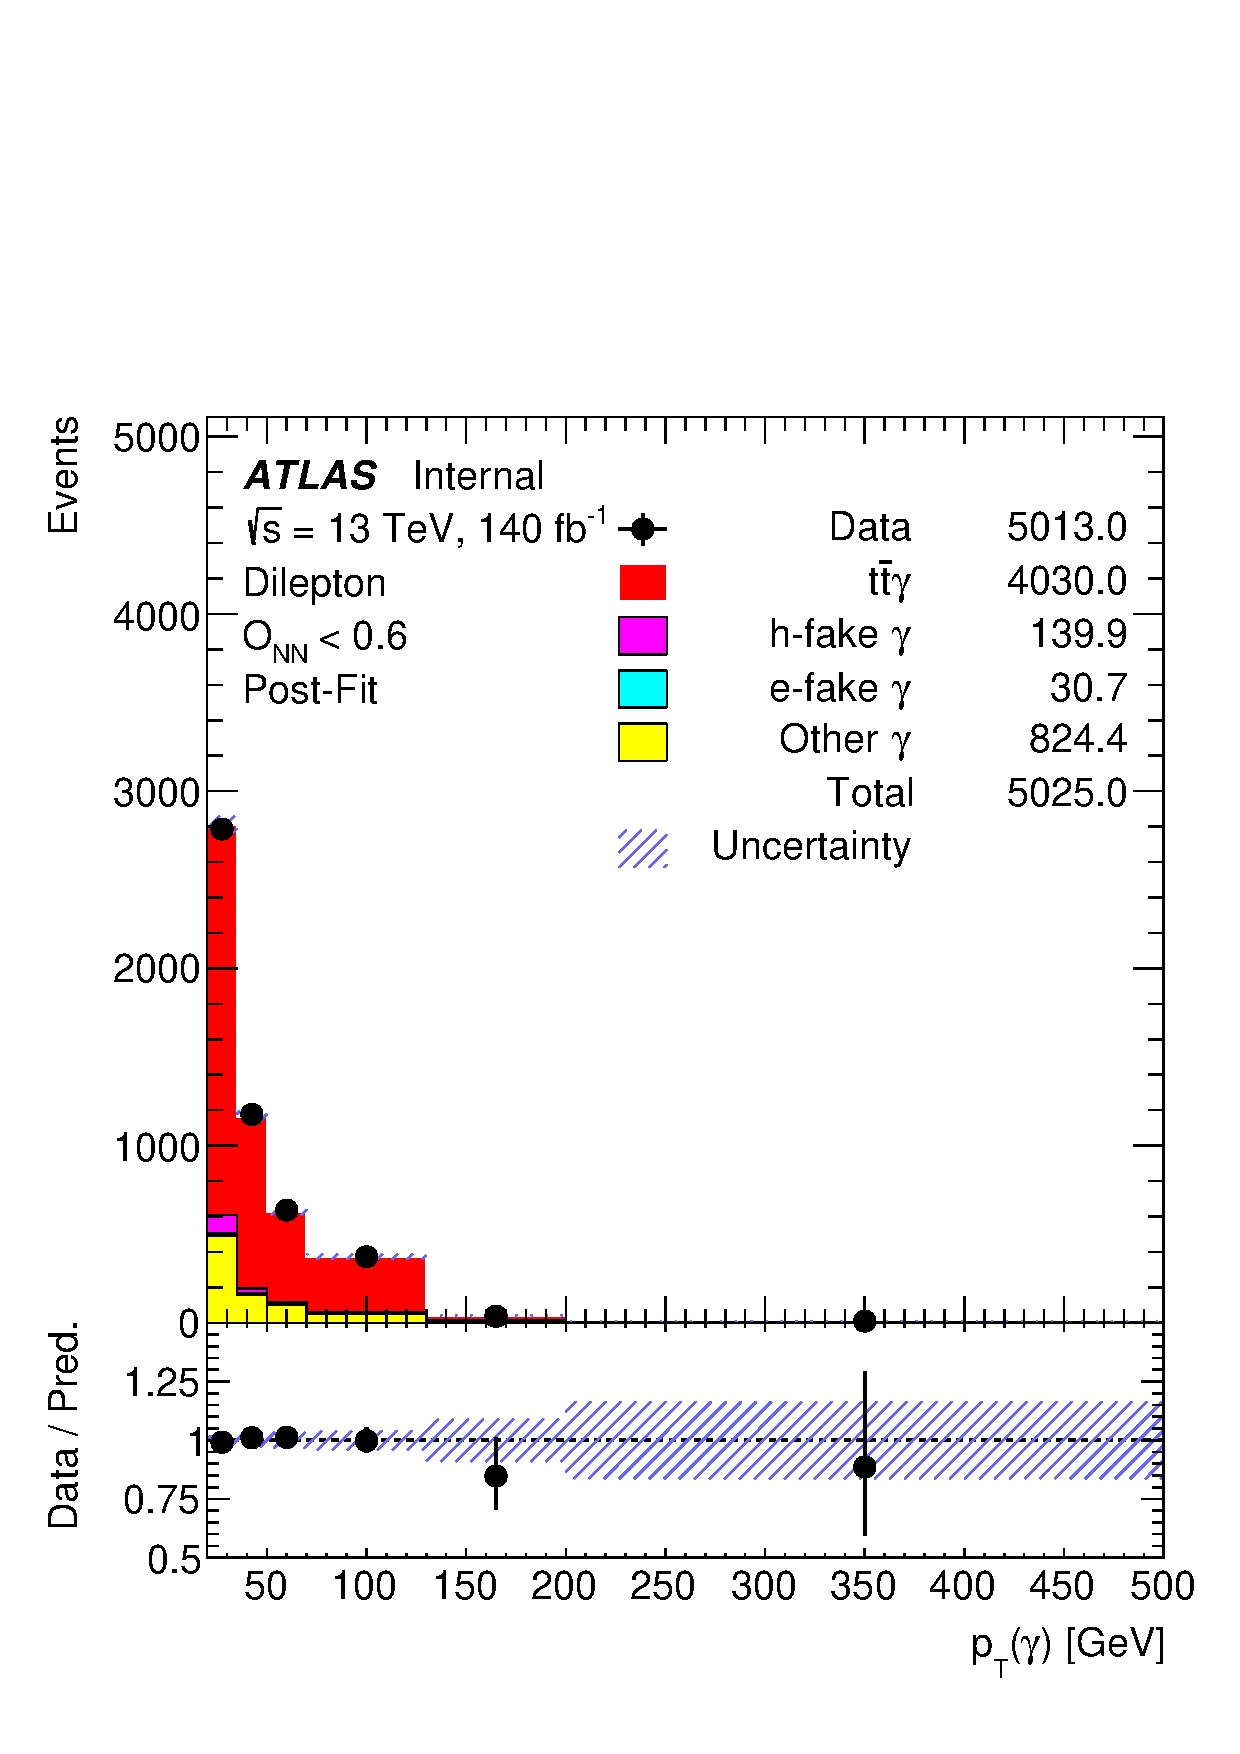
\includegraphics[width=0.30\textwidth]{figures/diff_xsec/dilep_tty_total/post_fit/tty2l_pt_all_syst/Plots/SR2_postFit.pdf}}
  \caption{The post-fit distributions of $p_T(\gamma)$ in two regions (based on the cut on the Neural Network output) (a) $O_{NN}>=0.6$ (b) $O_{NN}<0.6$ 
  in dilepton channel.}
  \label{fig:pt_postfit_dilep_tty_total_realdata}
\end{figure}




\begin{figure}[ht]
  \centering
  \subfloat[Part 1]{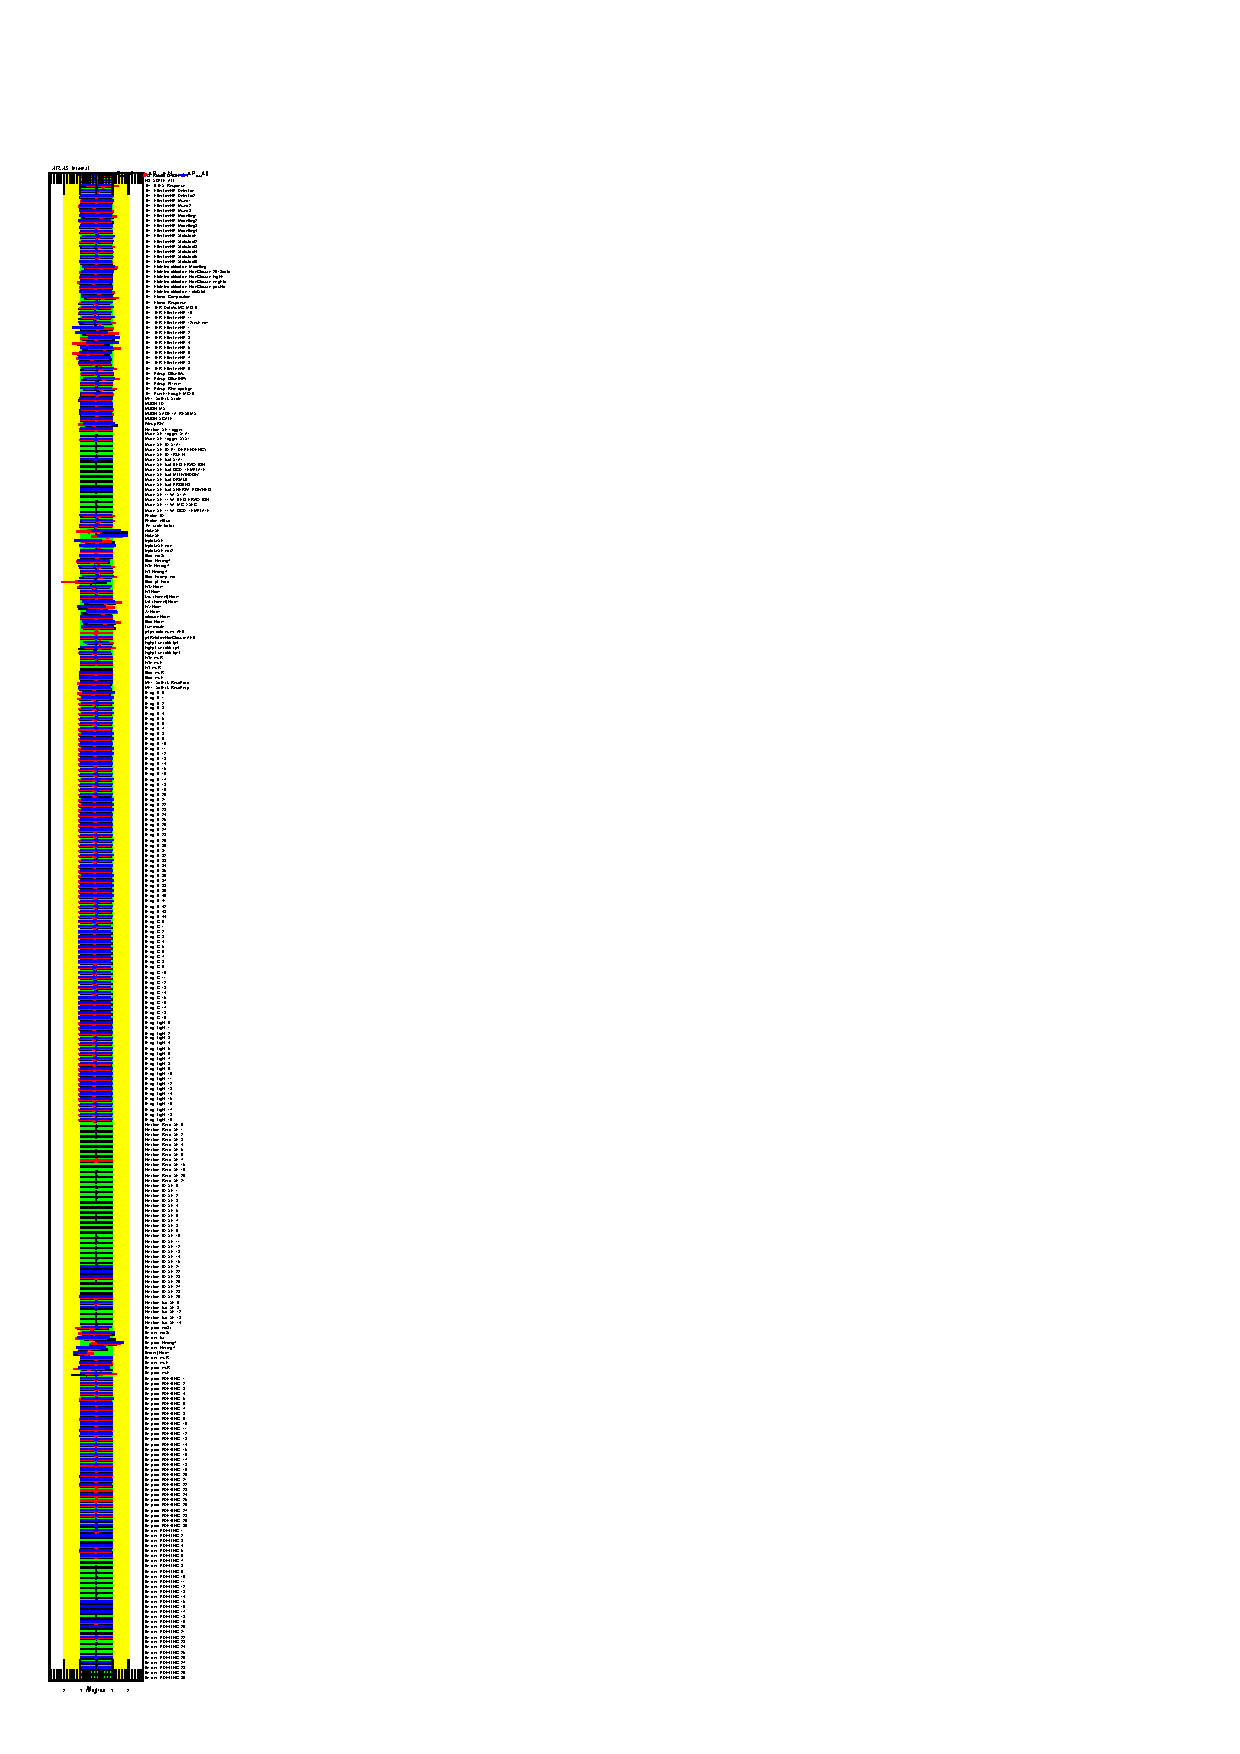
\includegraphics[width=0.40\textwidth, viewport=0 375 150 750, clip]{figures/diff_xsec/ljet_tty_total_mu_blinded/compare_NP_pulls/compare_NP_dilep_fits_drphb_drlj_dr/NuisPar_comp.pdf}}
  \quad
  \subfloat[Part 1]{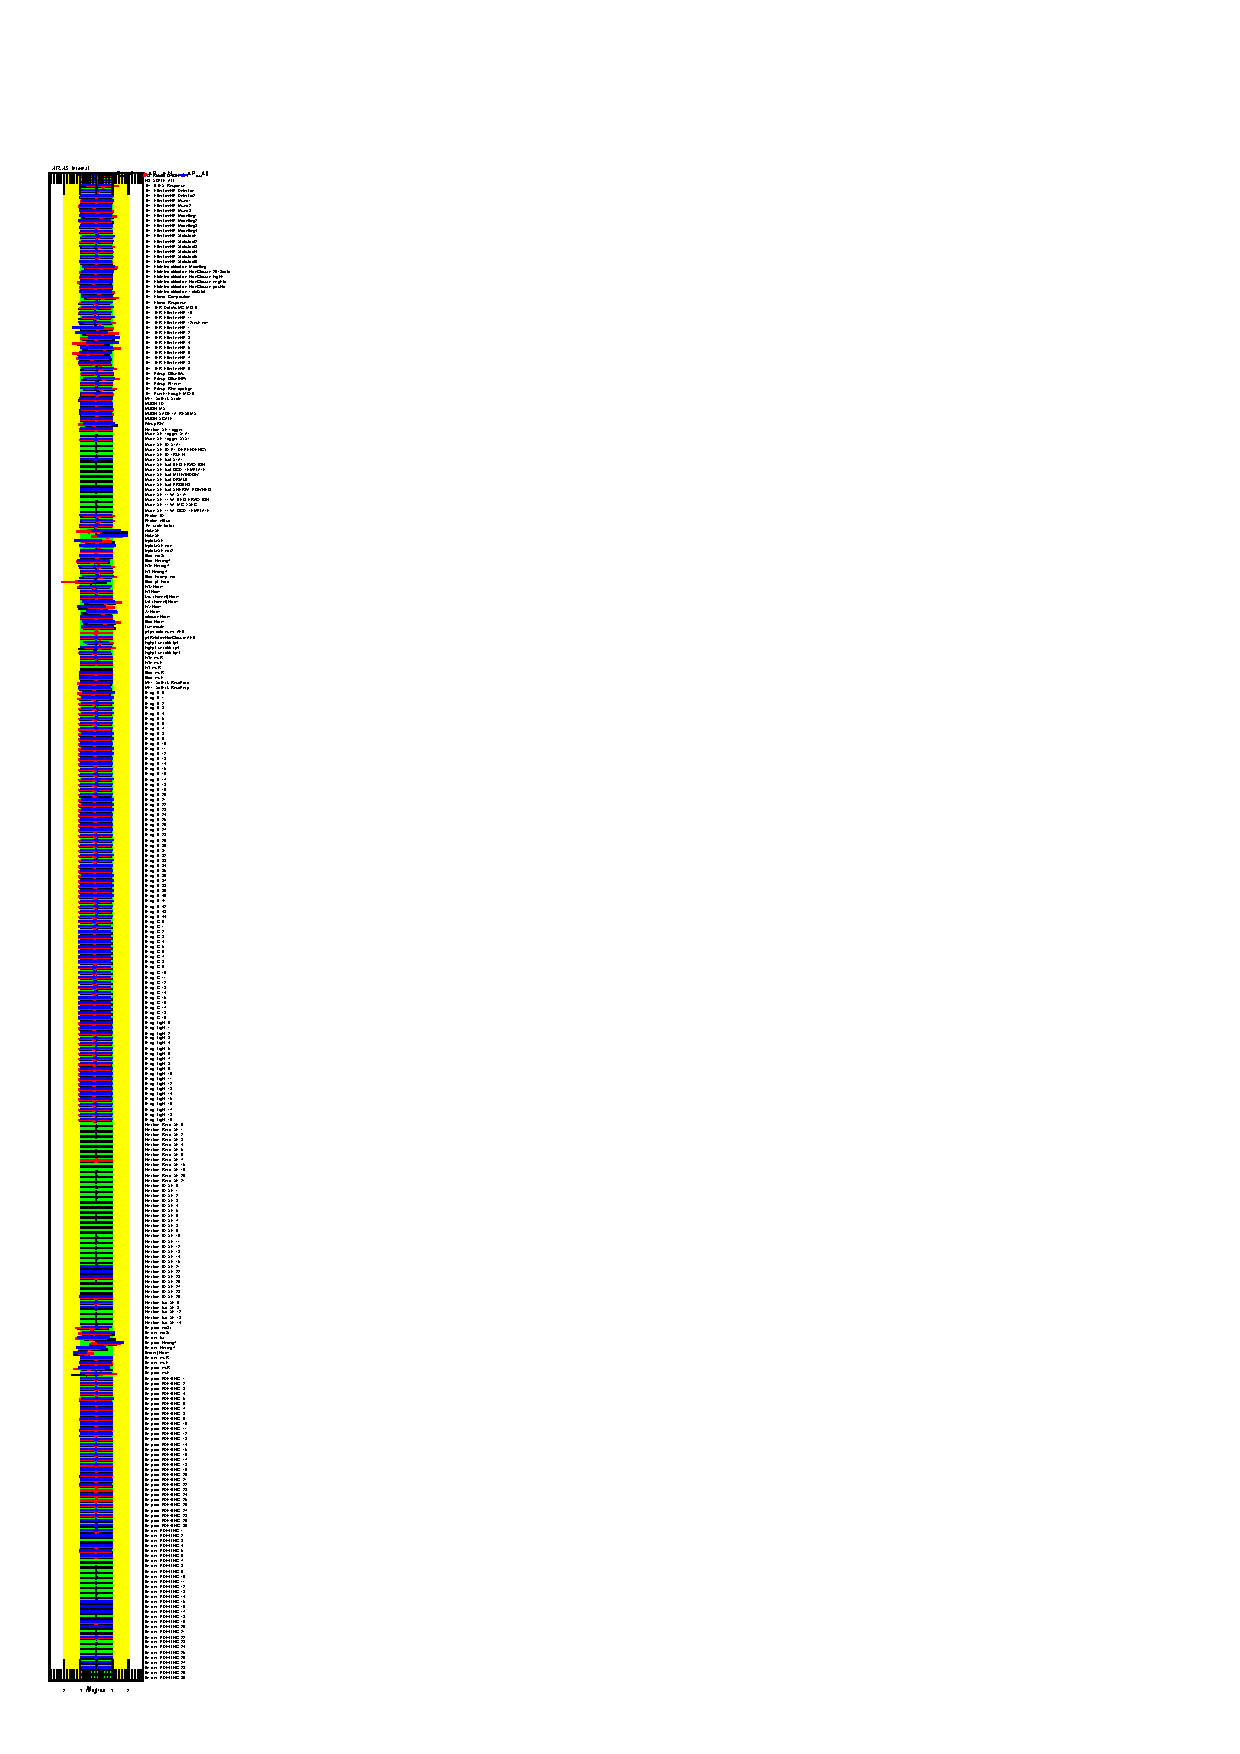
\includegraphics[width=0.40\textwidth, viewport=0 0 150 375, clip]{figures/diff_xsec/ljet_tty_total_mu_blinded/compare_NP_pulls/compare_NP_dilep_fits_drphb_drlj_dr/NuisPar_comp.pdf}}
  %\vspace{0.5cm}
  \caption{Pull plots obtained from the fit to the data for the single lepton channel, for the \tty (total) measurement.}
  \label{fig:pull_plot_pt_ljet_mu_blinded_tty_total}

\end{figure}
\FloatBarrier

\begin{figure}[ht]
  \centering
  \subfloat[Part 1]{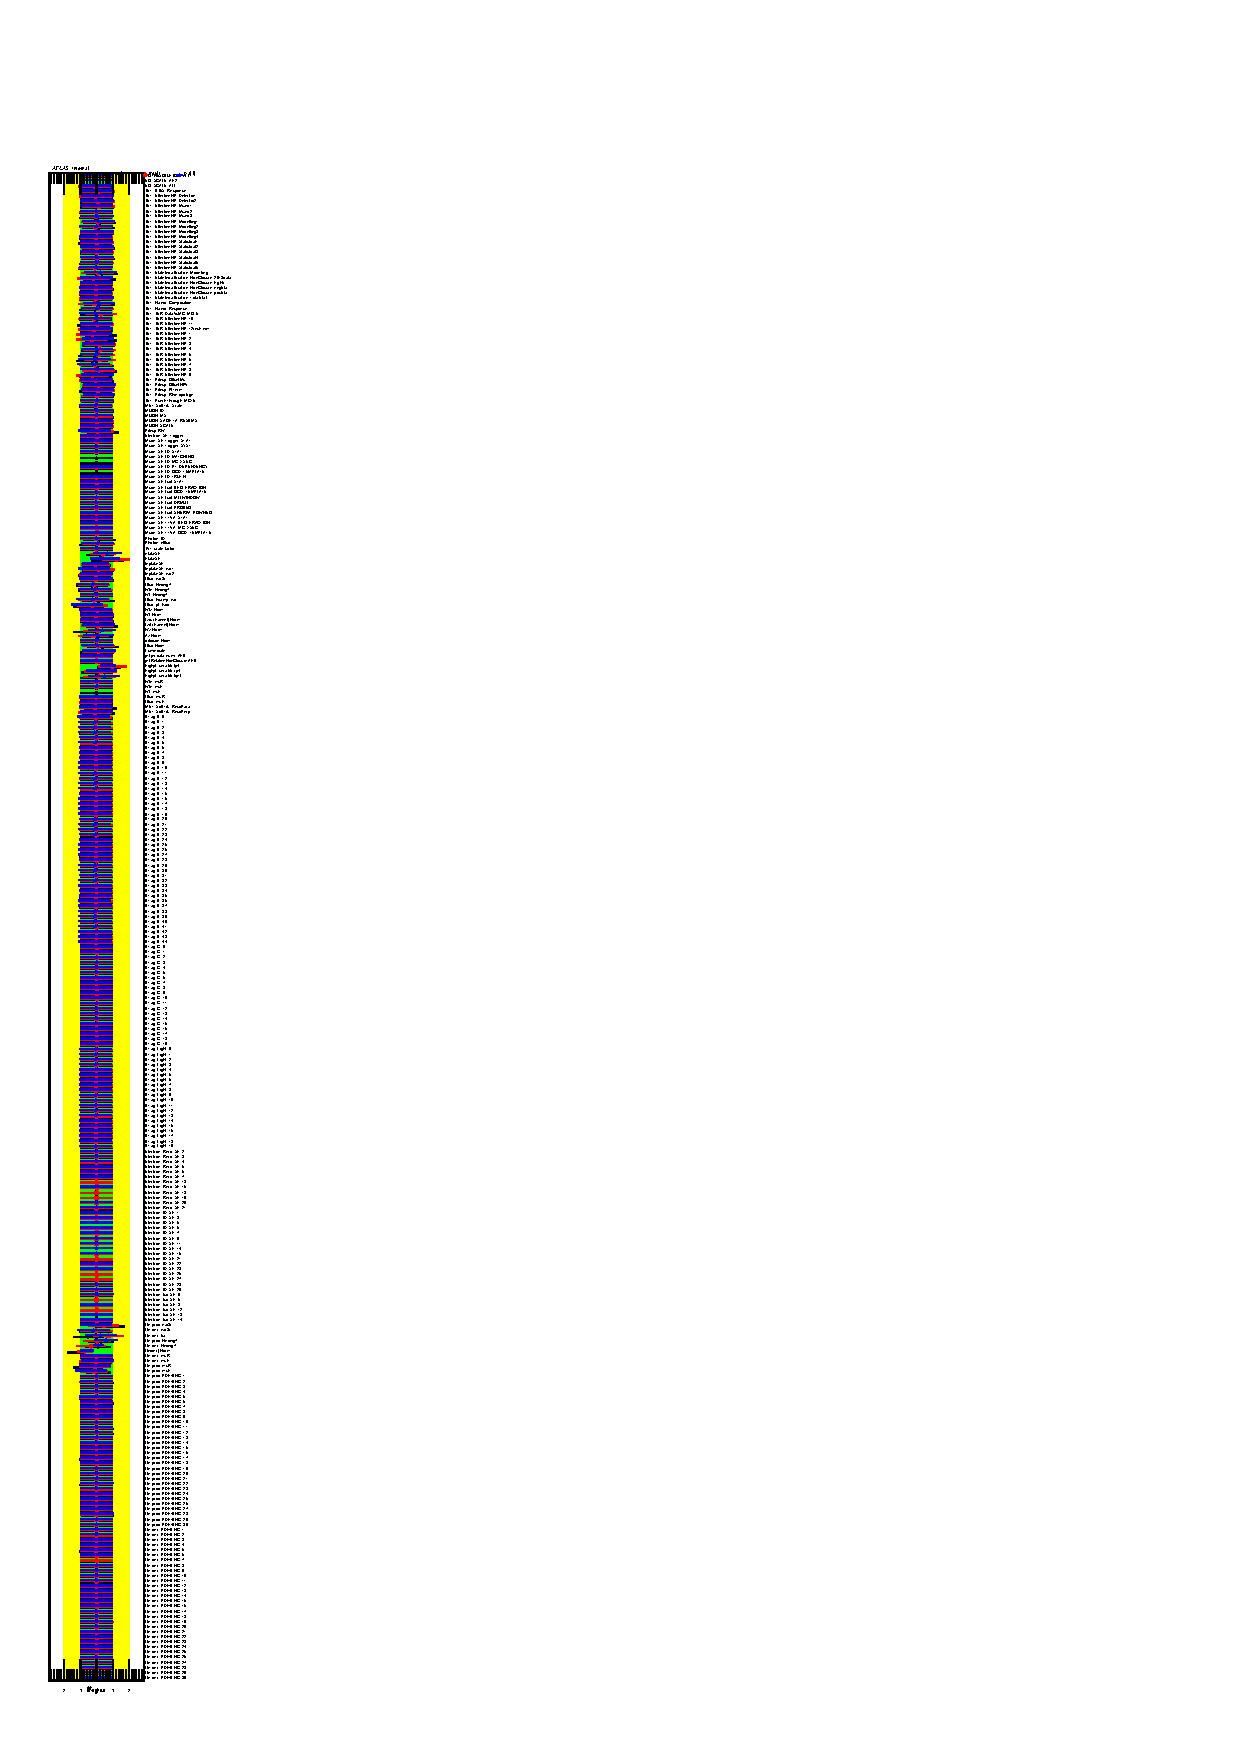
\includegraphics[width=0.40\textwidth, viewport=0 375 150 750, clip]{figures/diff_xsec/ljet_tty_total_mu_blinded/compare_NP_pulls/compare_NP_dilep_fits_pt_ptj1_eta/NuisPar_comp.pdf}}
  \quad
  \subfloat[Part 1]{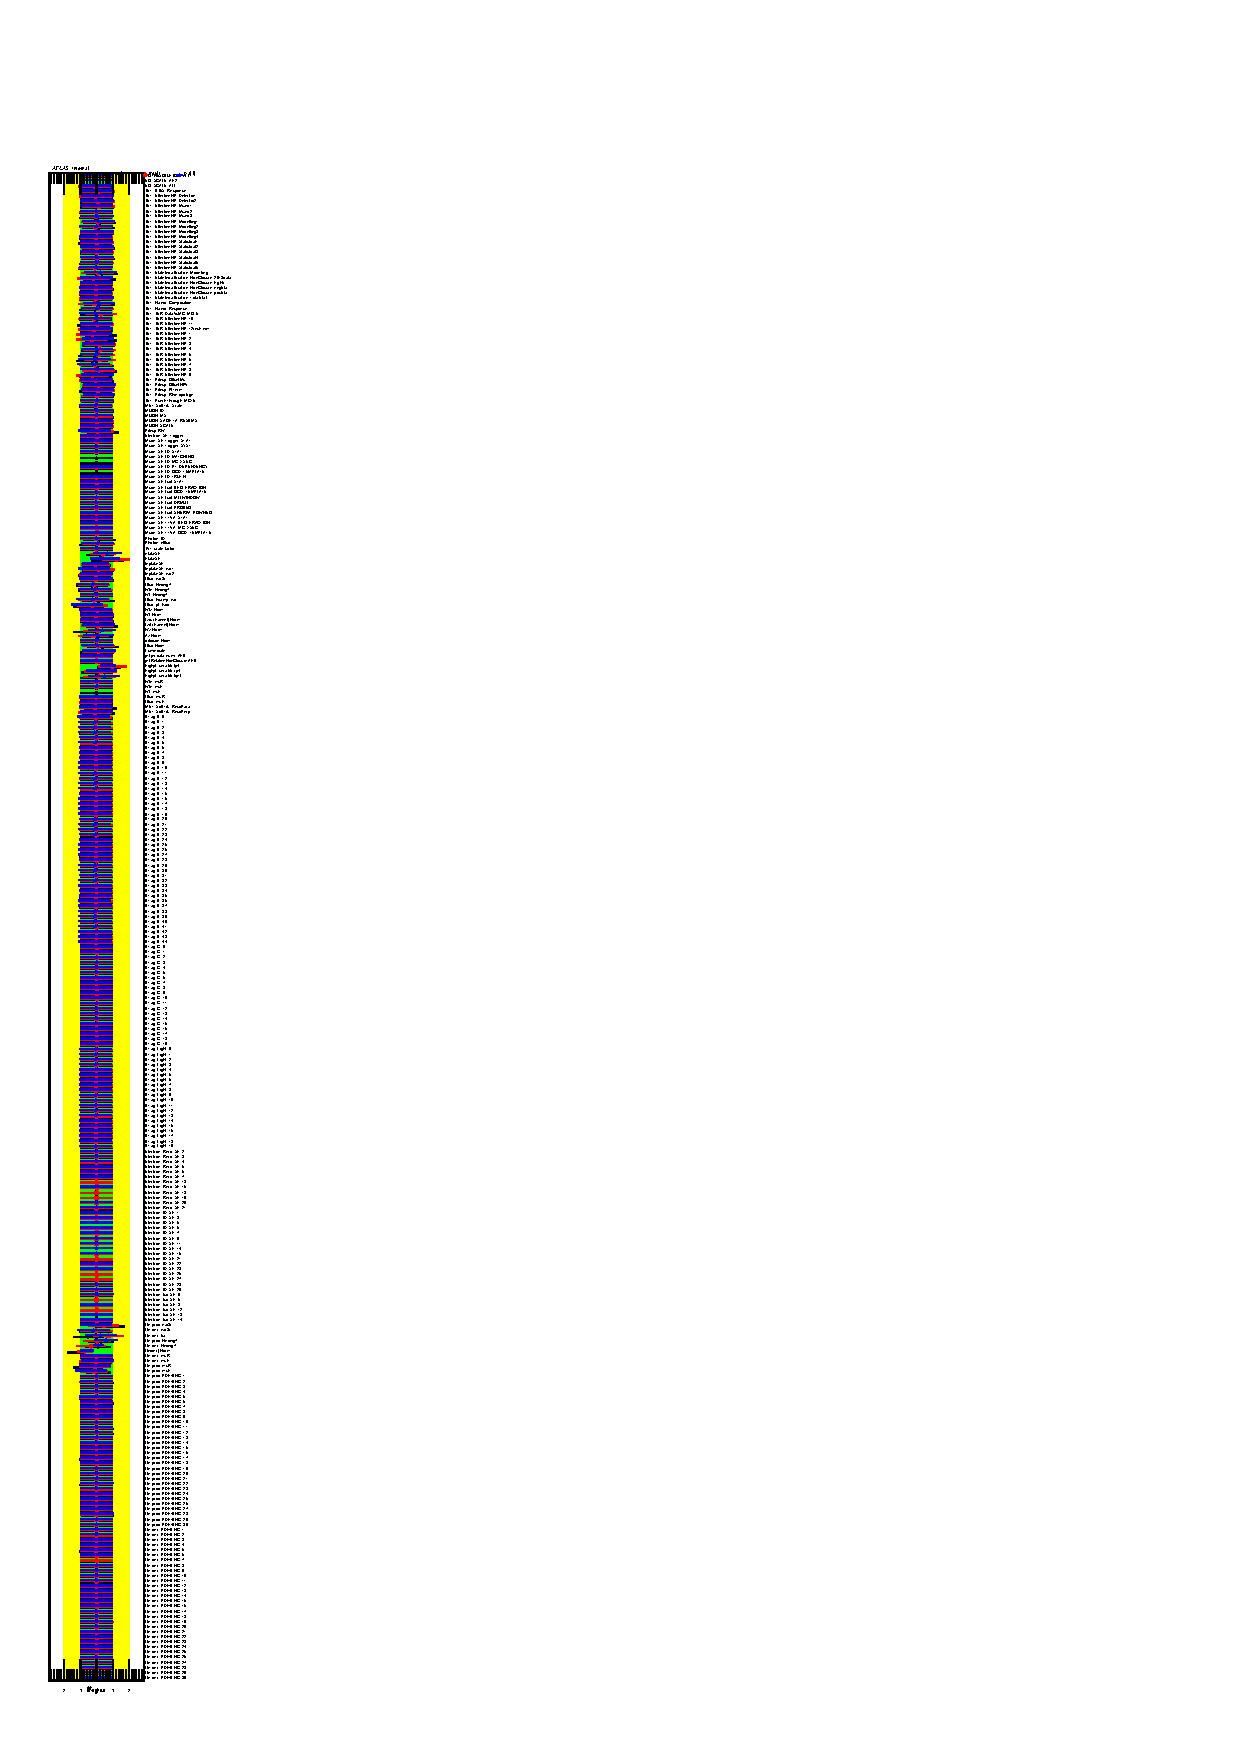
\includegraphics[width=0.40\textwidth, viewport=0 0 150 375, clip]{figures/diff_xsec/ljet_tty_total_mu_blinded/compare_NP_pulls/compare_NP_dilep_fits_pt_ptj1_eta/NuisPar_comp.pdf}}
  %\vspace{0.5cm}
  \caption{Pull plots obtained from the fit to the data for the single lepton channel, for the \tty (total) measurement.}
  \label{fig:pull_plot_pt_ljet_mu_blinded_tty_total}

\end{figure}
\FloatBarrier


%\begin{figure}[ht]
%  \centering
%  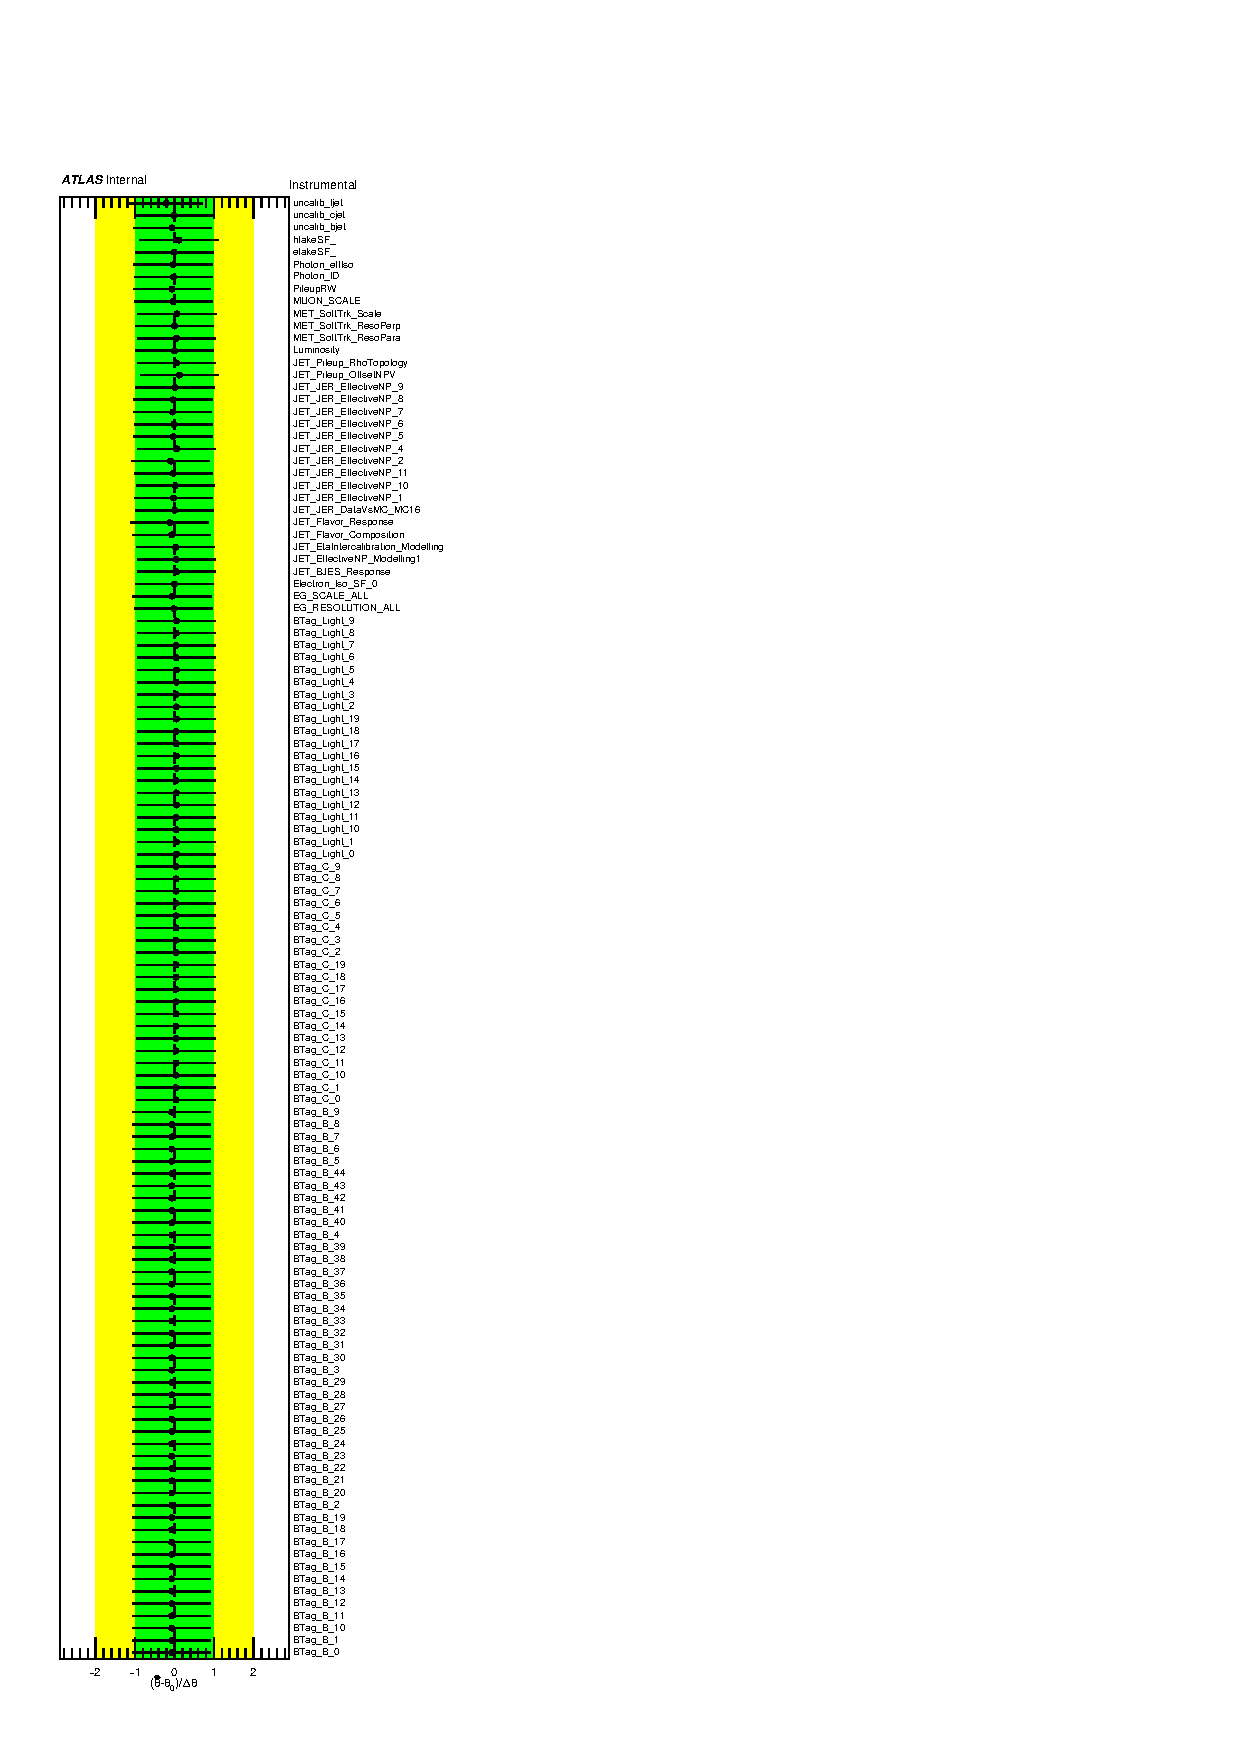
\includegraphics[width=0.25\textwidth]{figures/diff_xsec/dilep_tty_total_mu_blinded/NPs/tty2l_pt_all_syst/NuisPar_Instrumental.pdf}
%  \quad \quad
%  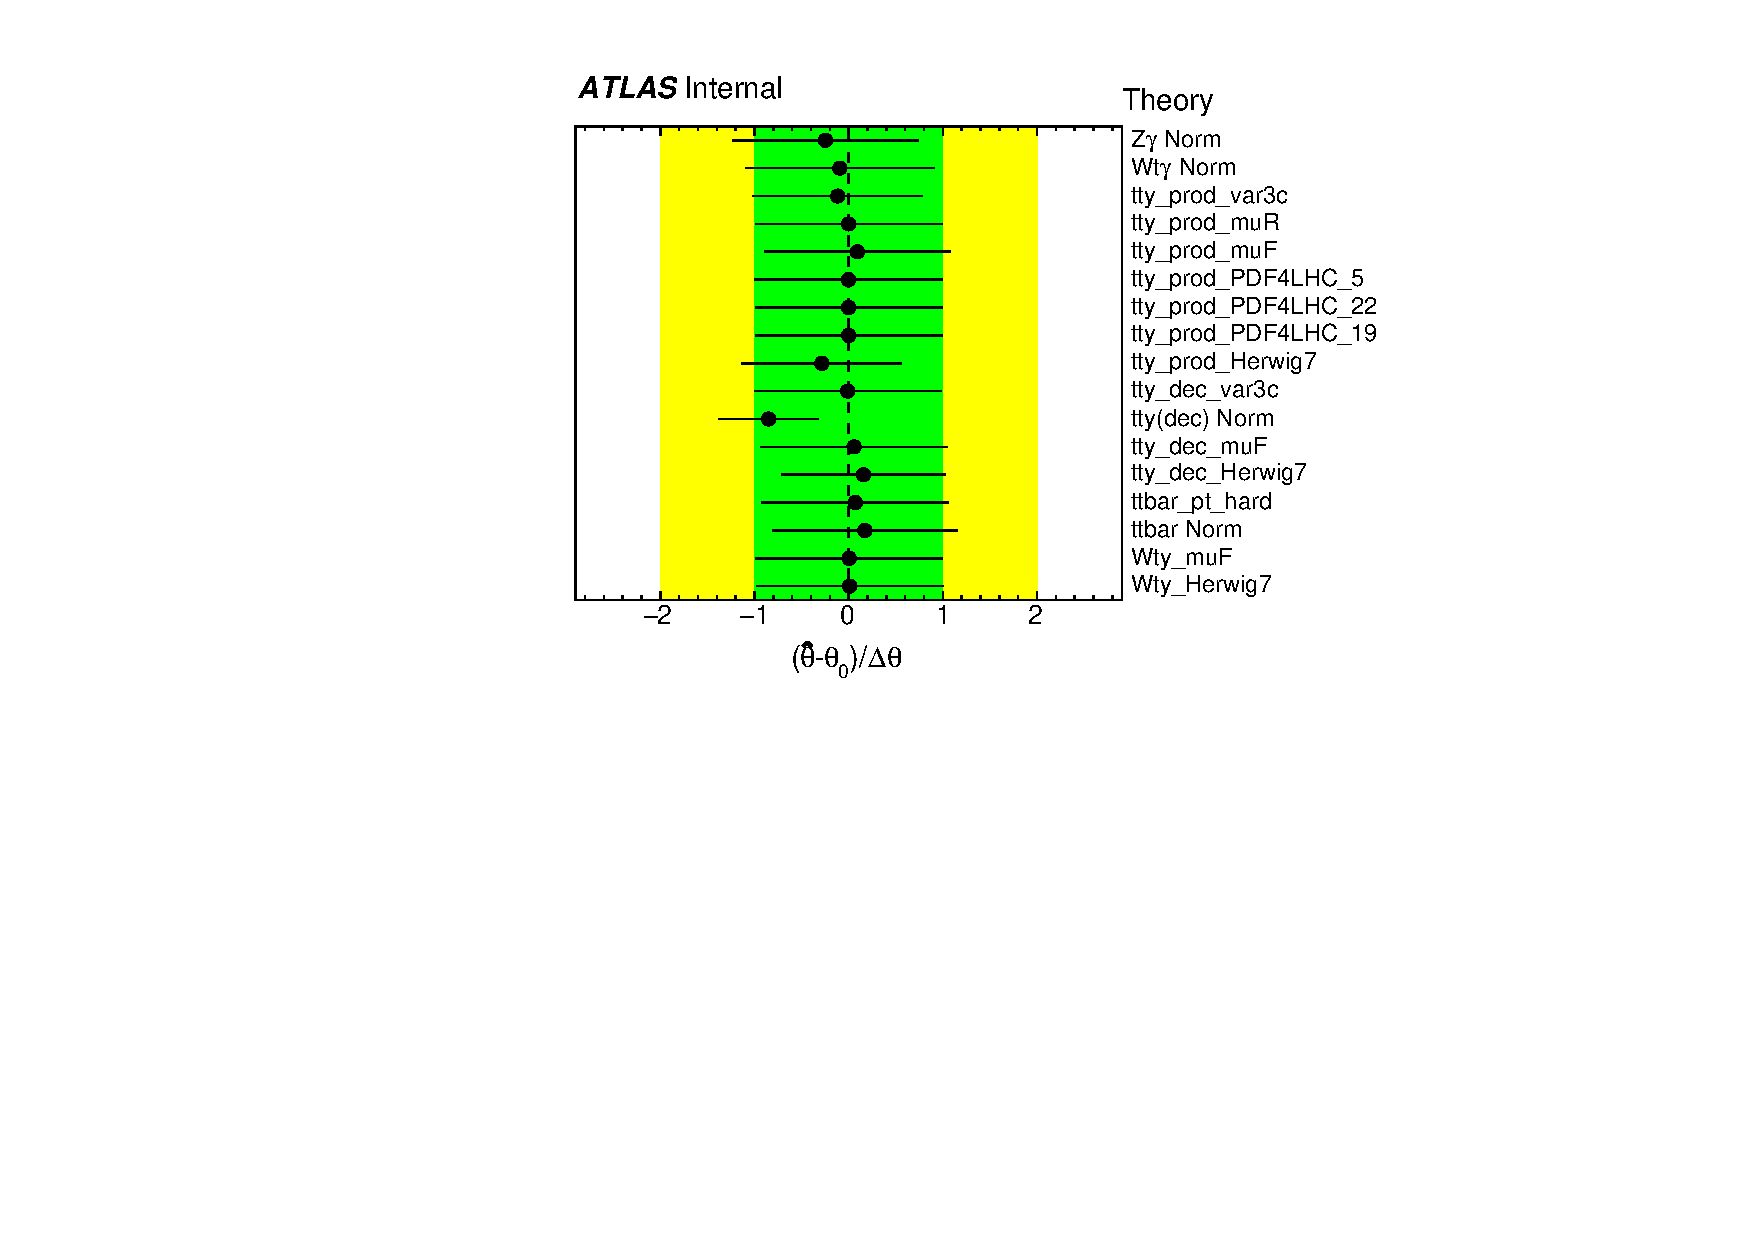
\includegraphics[width=0.25\textwidth]{figures/diff_xsec/dilep_tty_total_mu_blinded/NPs/tty2l_pt_all_syst/NuisPar_Theory.pdf}
%  \quad\quad
%  %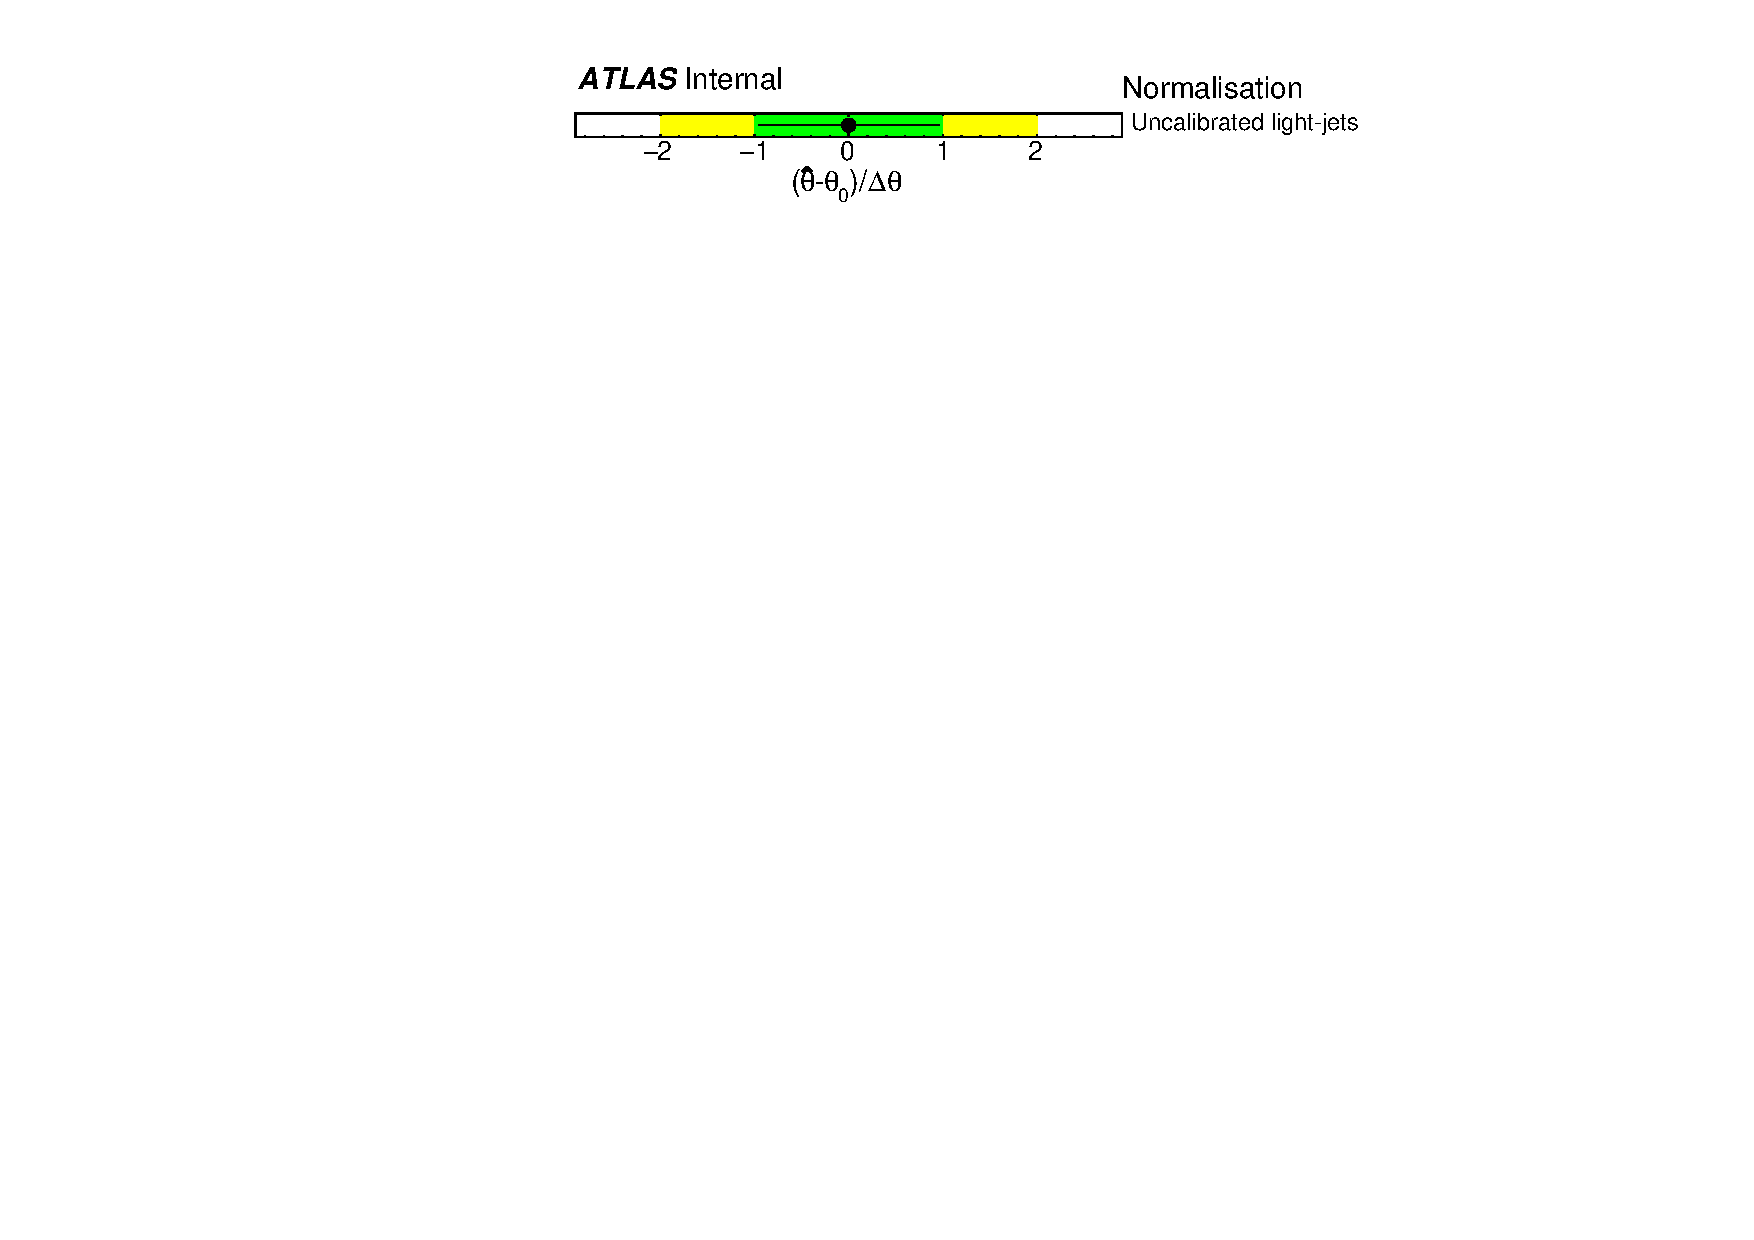
\includegraphics[width=0.25\textwidth]{figures/diff_xsec/dilep_tty_total_mu_blinded/NPs/tty2l_pt_all_syst/NuisPar_Normalisation.pdf}
%  \caption{Pull plots obtained from the fit to the data for the dilepton channel}
%  \label{fig:pull_plot_pt_dilep_mu_blinded_1_tty_total}
%\end{figure}
%\FloatBarrier


\begin{figure}[ht]
  \centering
  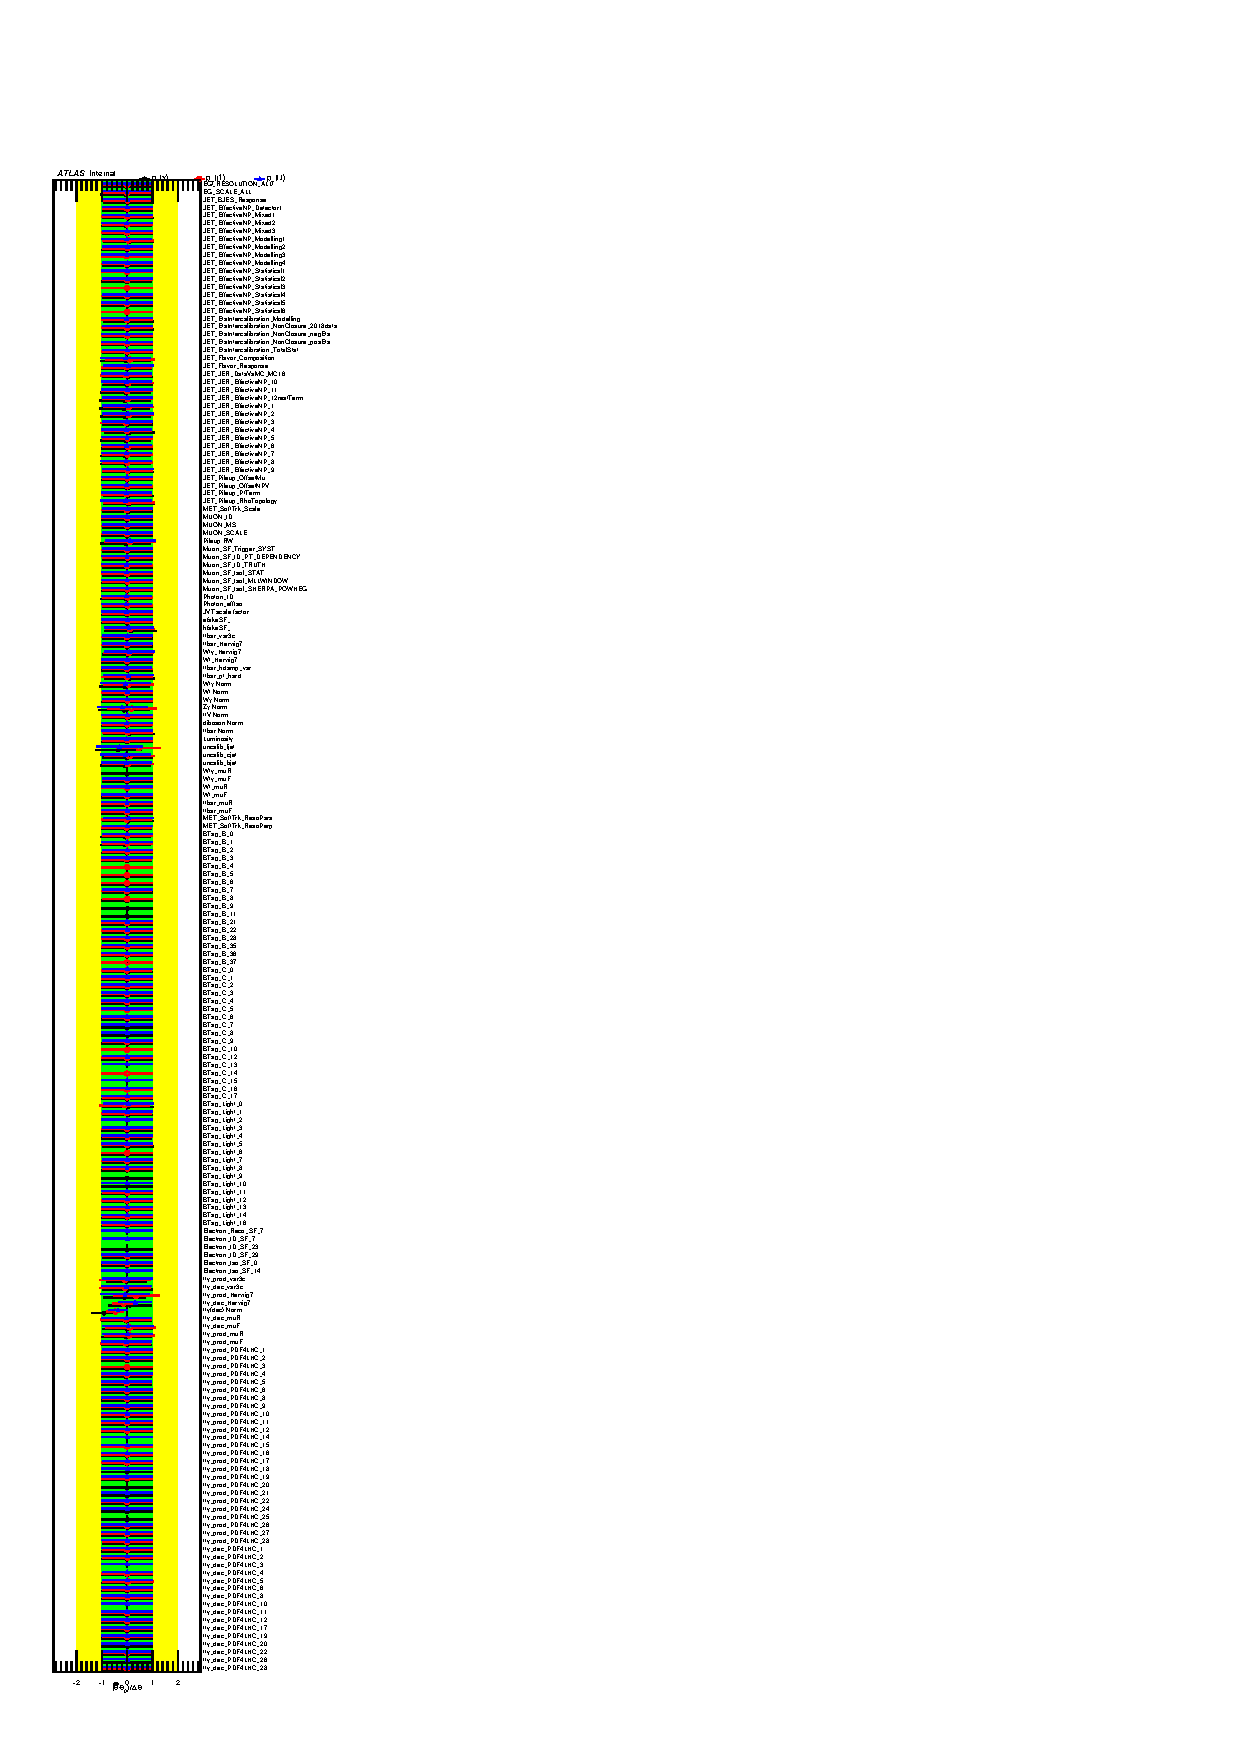
\includegraphics[width=0.22\textwidth]{figures/diff_xsec/dilep_tty_total_mu_blinded/compare_NP_pulls/compare_NP_dilep_fits_pt_ptj1_ptll/NuisPar_comp.pdf}
  \quad \quad
  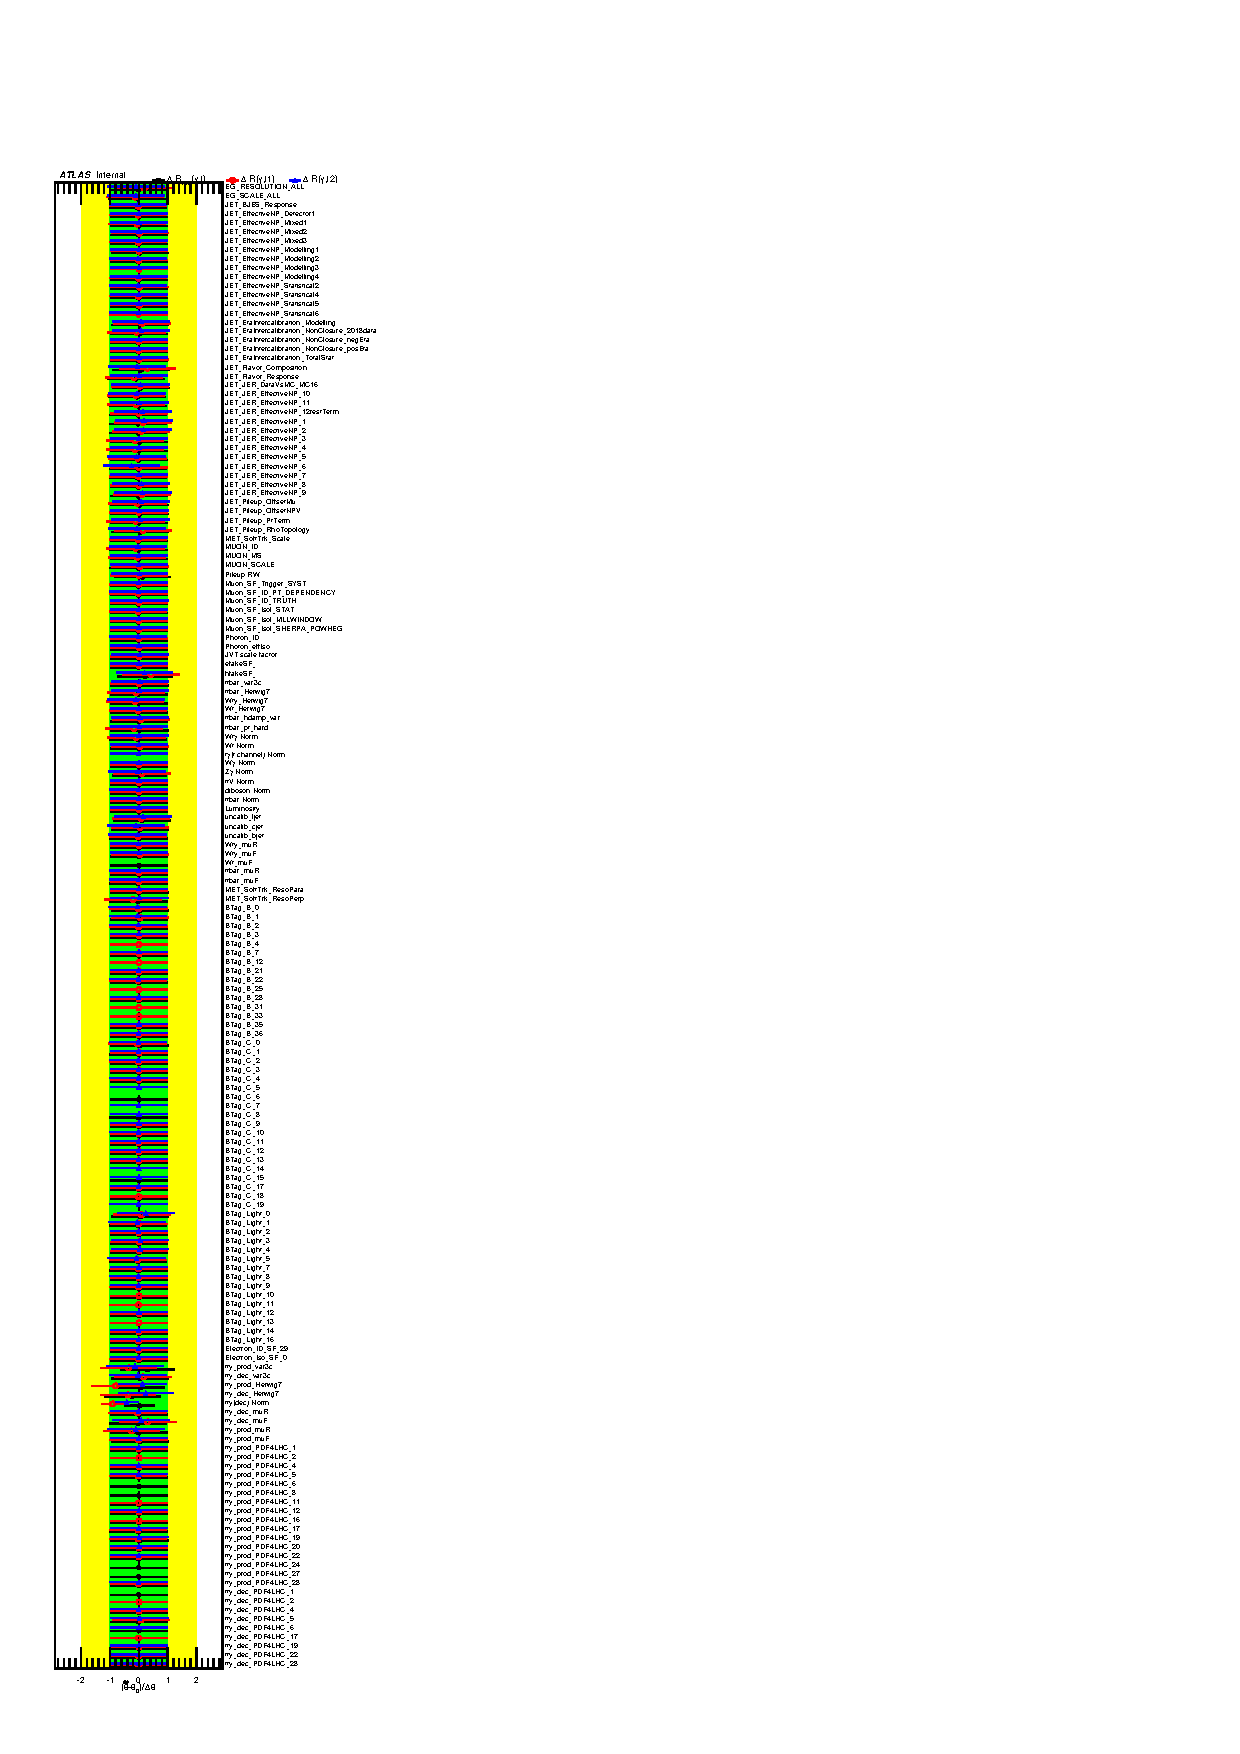
\includegraphics[width=0.22\textwidth]{figures/diff_xsec/dilep_tty_total_mu_blinded/compare_NP_pulls/compare_NP_dilep_fits_dr_dr1_dr2/NuisPar_comp.pdf}
  %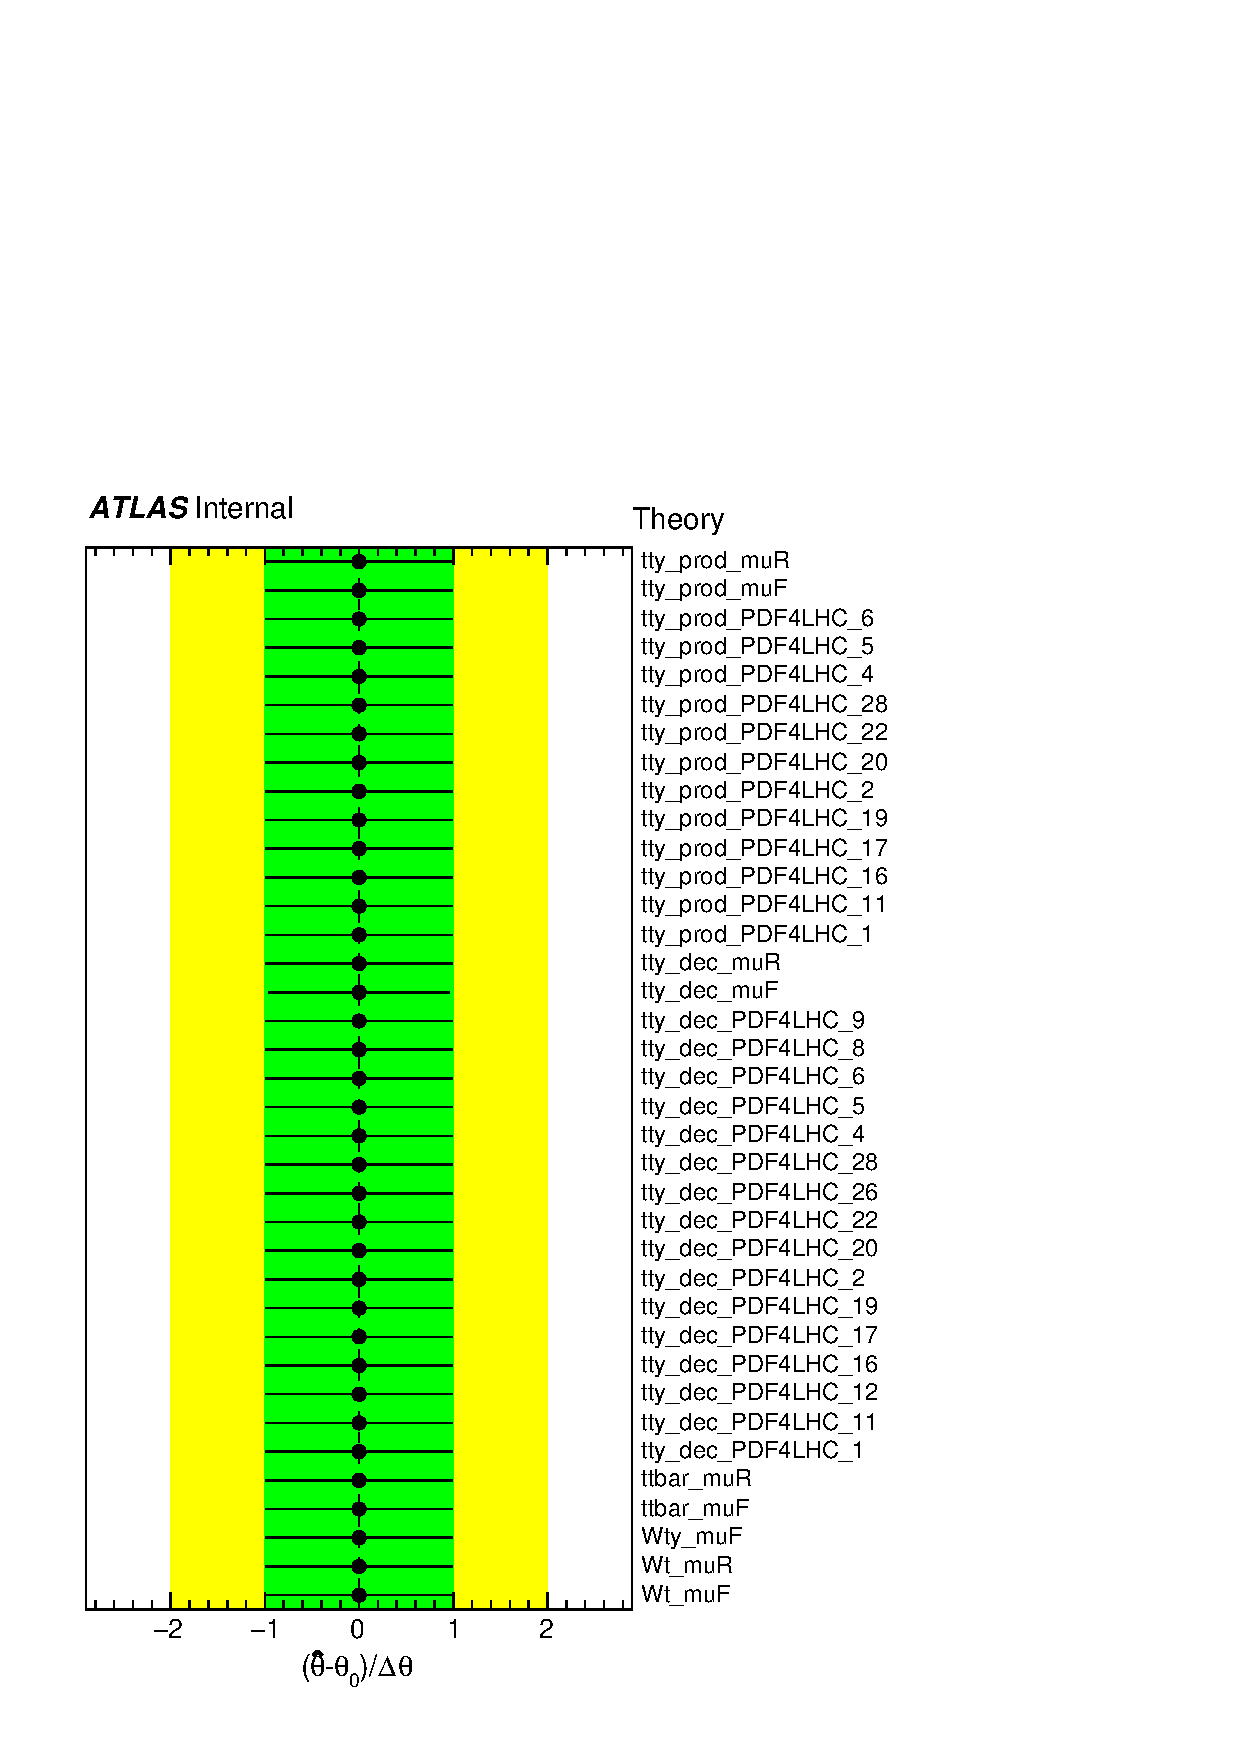
\includegraphics[width=0.32\textwidth]{figures/diff_xsec/dilep/Unfolded_data_tty_dec_free_mu_blinded/compare_NP_dilep_fits_pt_ptj1_ptll/NuisPar_Theory.pdf}
  \caption{Pull plots obtained from the fit to the data for the dilepton channel, for the \tty (total) measurement.}
  \label{fig:pull_plot_pt_dilep_mu_blinded_1_tty_total}
\end{figure}
\FloatBarrier

\begin{figure}[ht]
  \centering
  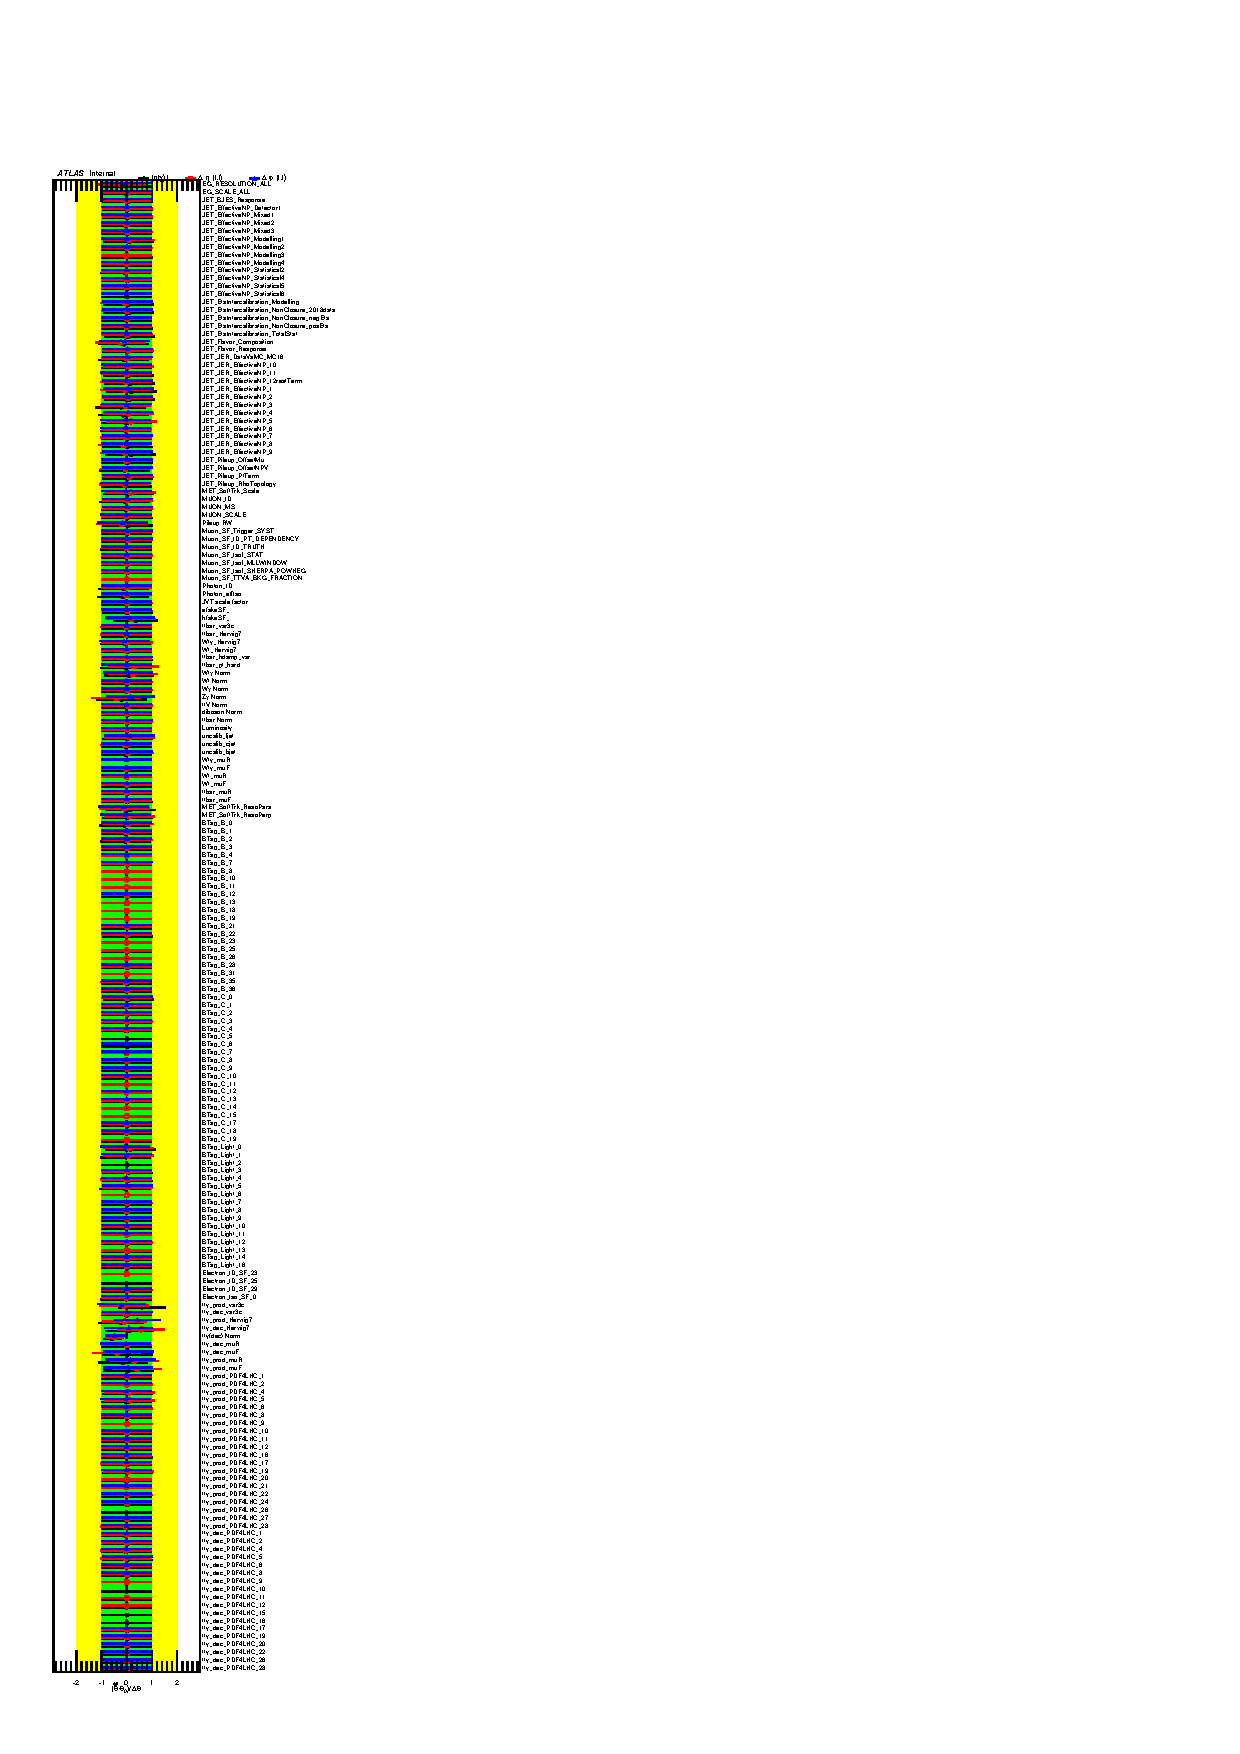
\includegraphics[width=0.22\textwidth]{figures/diff_xsec/dilep_tty_total_mu_blinded/compare_NP_pulls/compare_NP_dilep_fits_detall_dphill_eta/NuisPar_comp.pdf}
  \quad \quad
  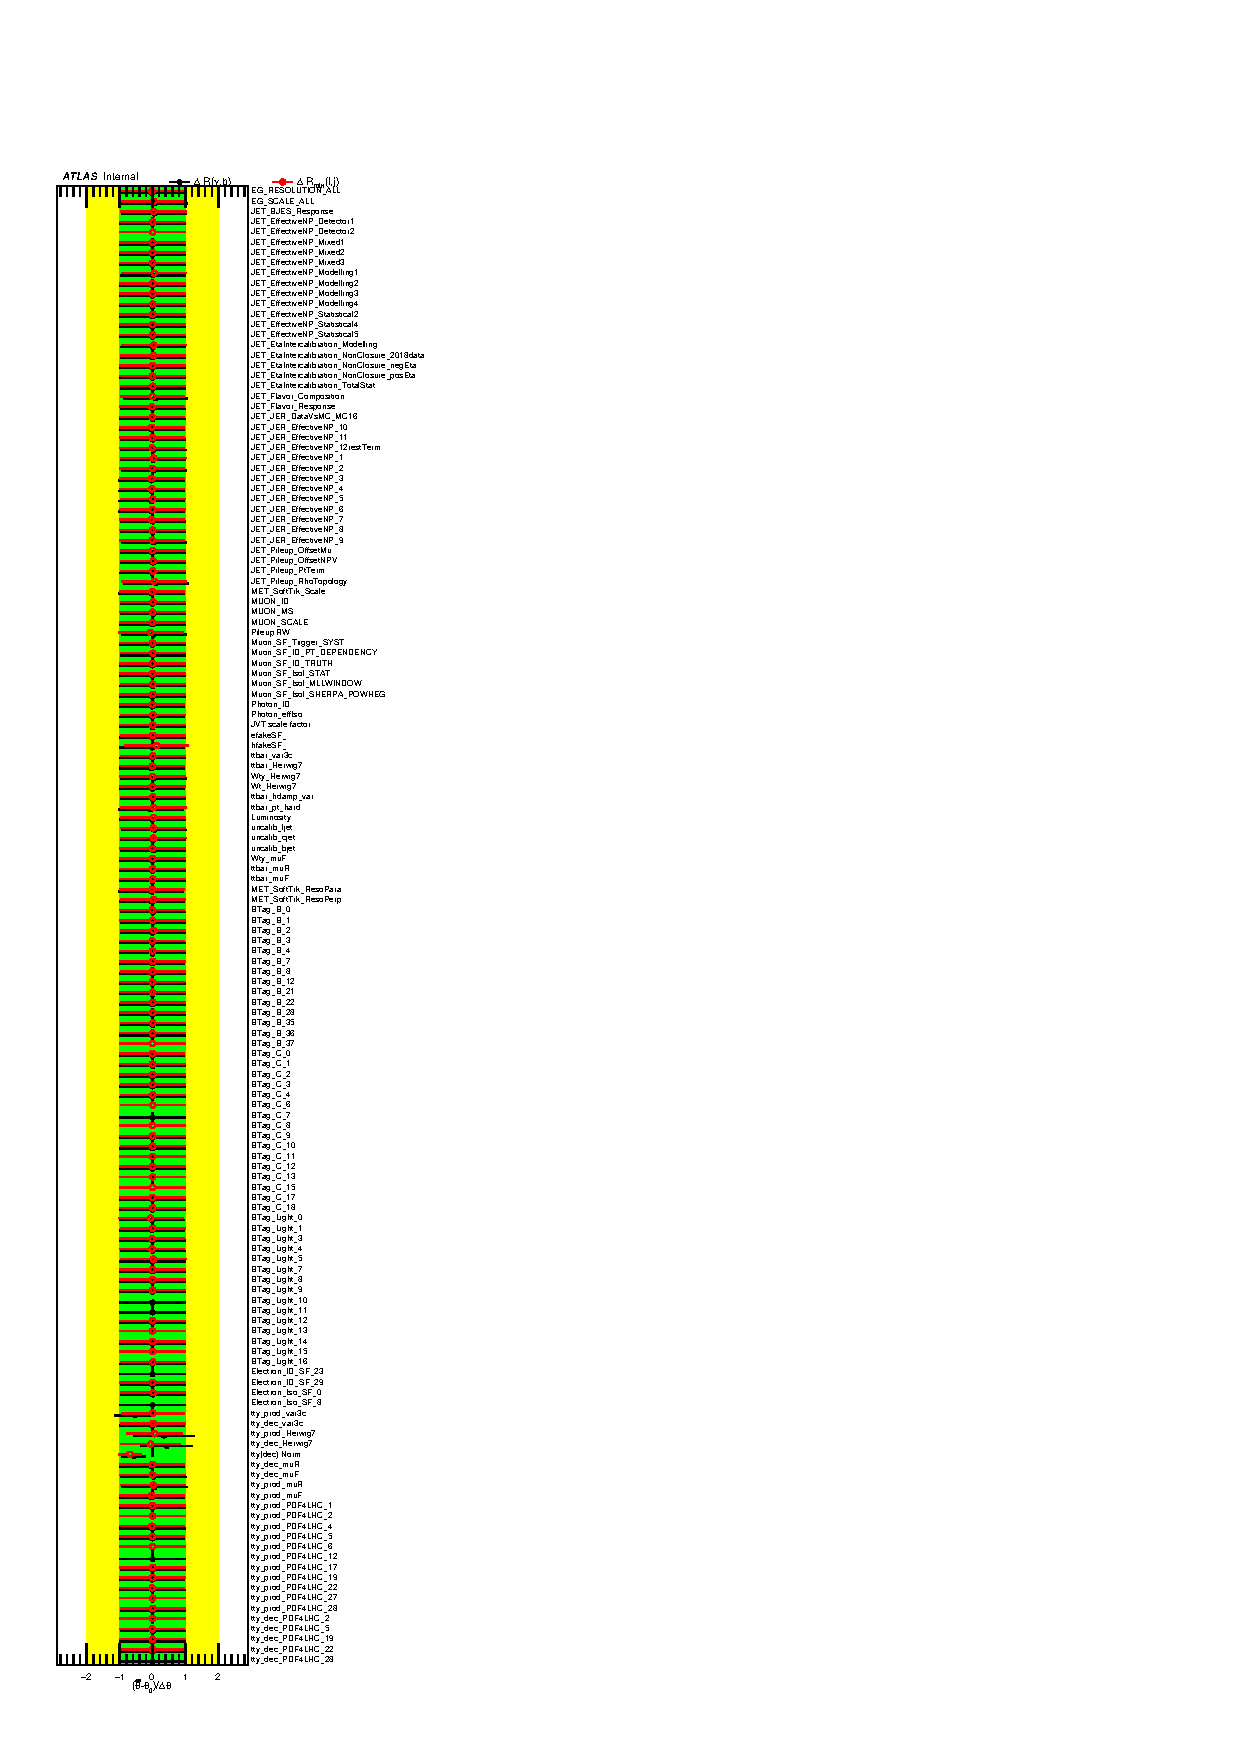
\includegraphics[width=0.22\textwidth]{figures/diff_xsec/dilep_tty_total_mu_blinded/compare_NP_pulls/compare_NP_dilep_fits_drphb_drlj/NuisPar_comp.pdf}
  \caption{Pull plots obtained from the fit to the data for the dilepton channel, for the \tty (total) measurement.}
  \label{fig:pull_plot_pt_dilep_mu_blinded_2_tty_total}
\end{figure}
\FloatBarrier


\begin{figure}[ht]
  \centering
  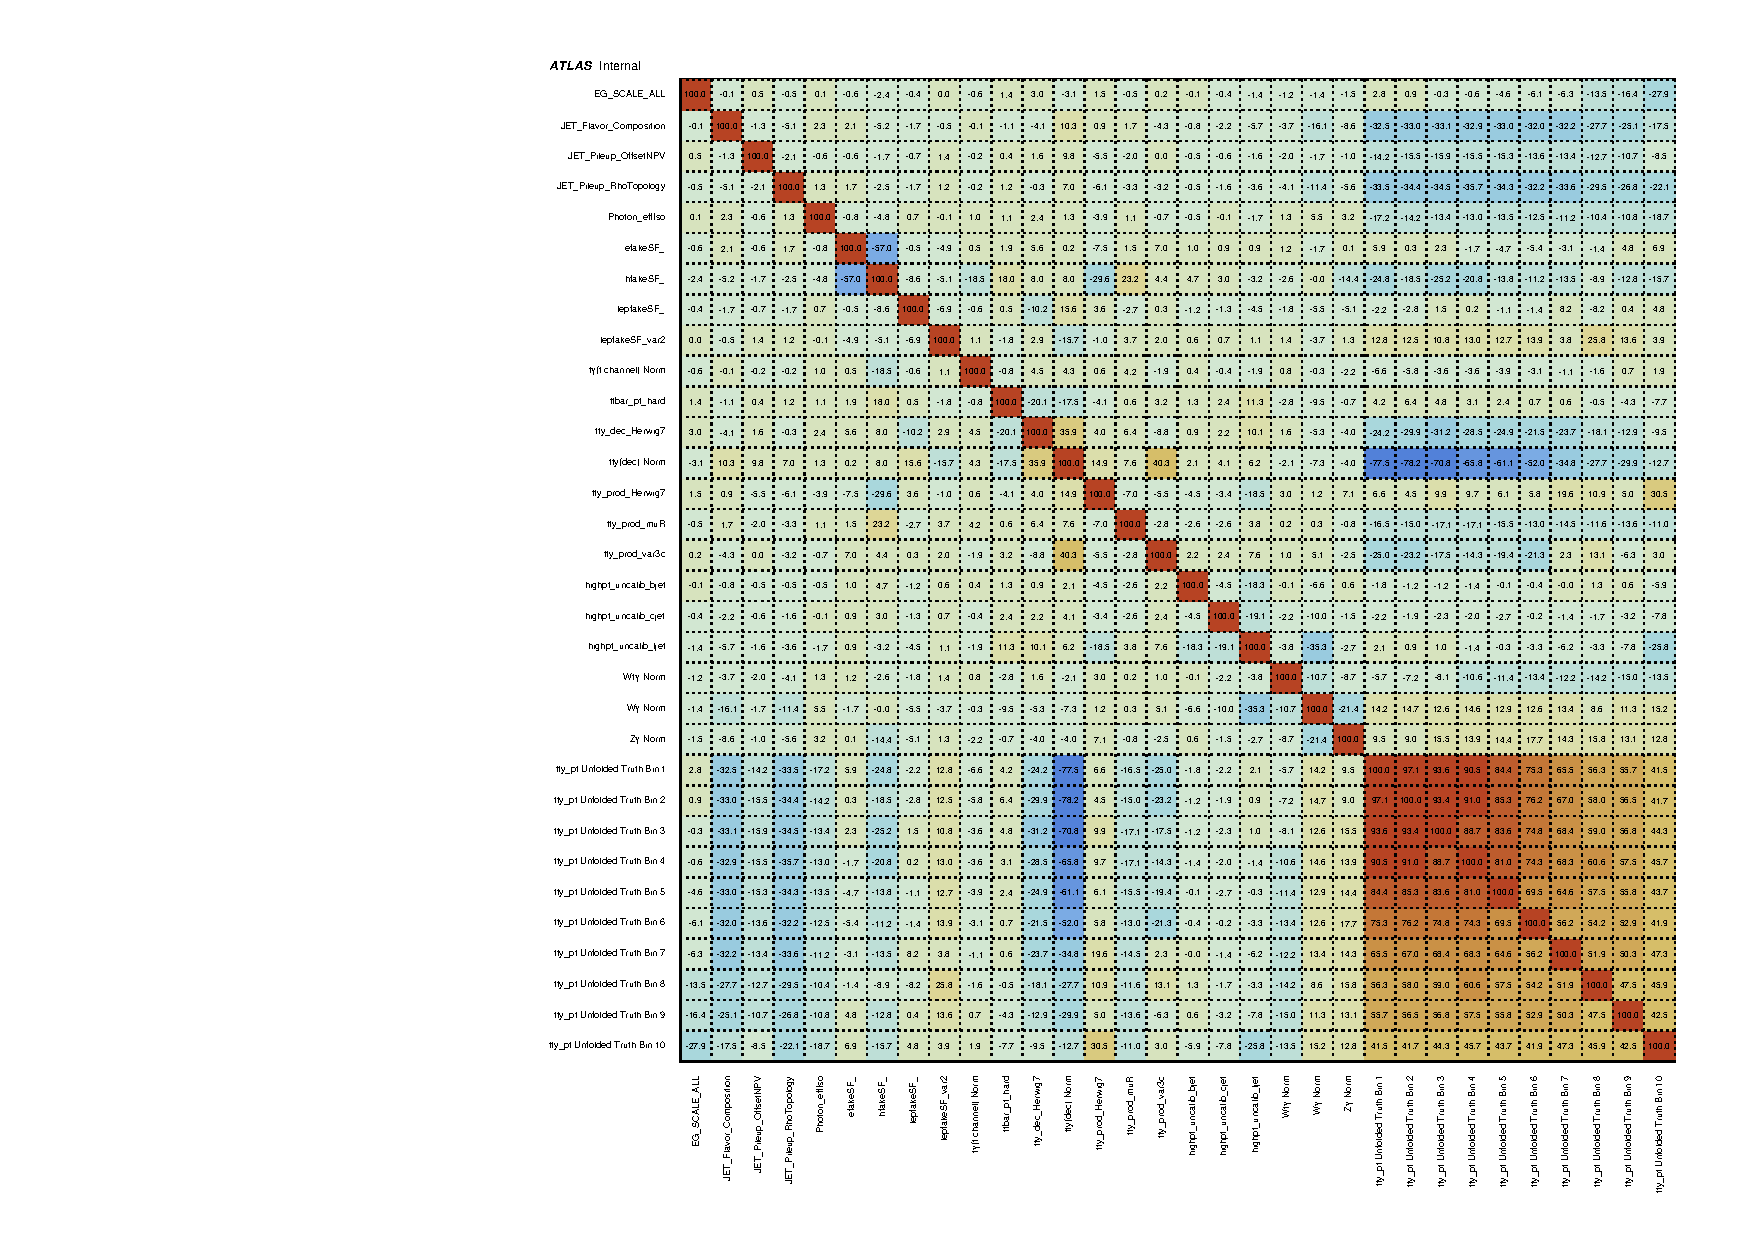
\includegraphics[width=0.8\textwidth]{figures/diff_xsec/ljet_tty_total_mu_blinded/correlations/tty1l_pt_all_syst/CorrMatrix.pdf}
  \caption{The correlation between the NPs and POIs for the measurement of 
  the $p_T(\gamma)$ distribution in single lepton channel for the \tty (total) measurement.}
  \label{fig:NP-corr_ljet_mu_blinded_tty_total}
\end{figure}
\FloatBarrier


\begin{figure}[ht]
  \centering
  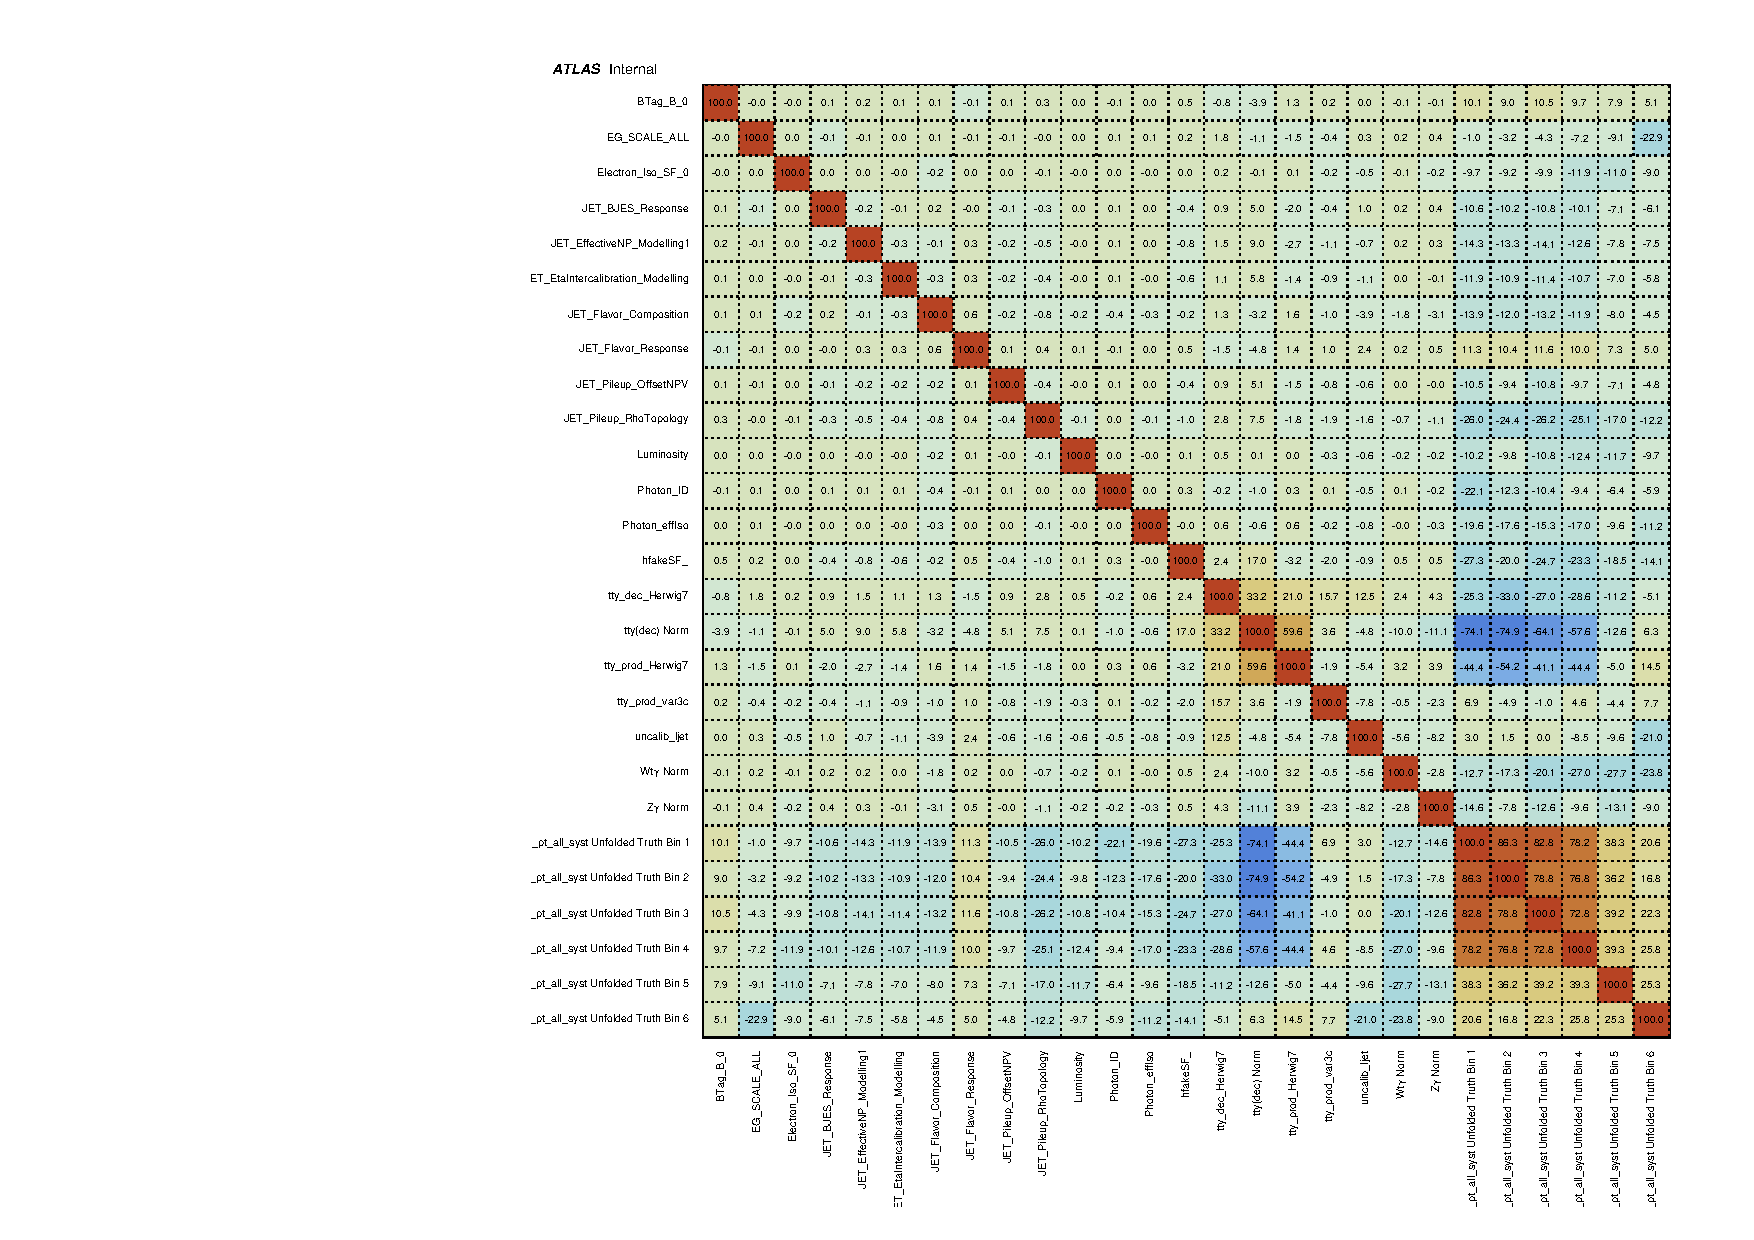
\includegraphics[width=0.8\textwidth]{figures/diff_xsec/dilep_tty_total_mu_blinded/correlations/tty2l_pt_all_syst/CorrMatrix.pdf}
  \caption{The correlation between the NPs and POIs for the measurement of 
  the $p_T(\gamma)$ distribution in dilepton channel for the \tty(total) measurement.}
  \label{fig:NP-corr_dilep_mu_blinded_tty_total}
\end{figure}
\FloatBarrier

%%%%%%%%%%%% RANKING %%%%%%%%%%%%%%%%%%%

\begin{figure}[ht]
  \centering
  \subfloat[]{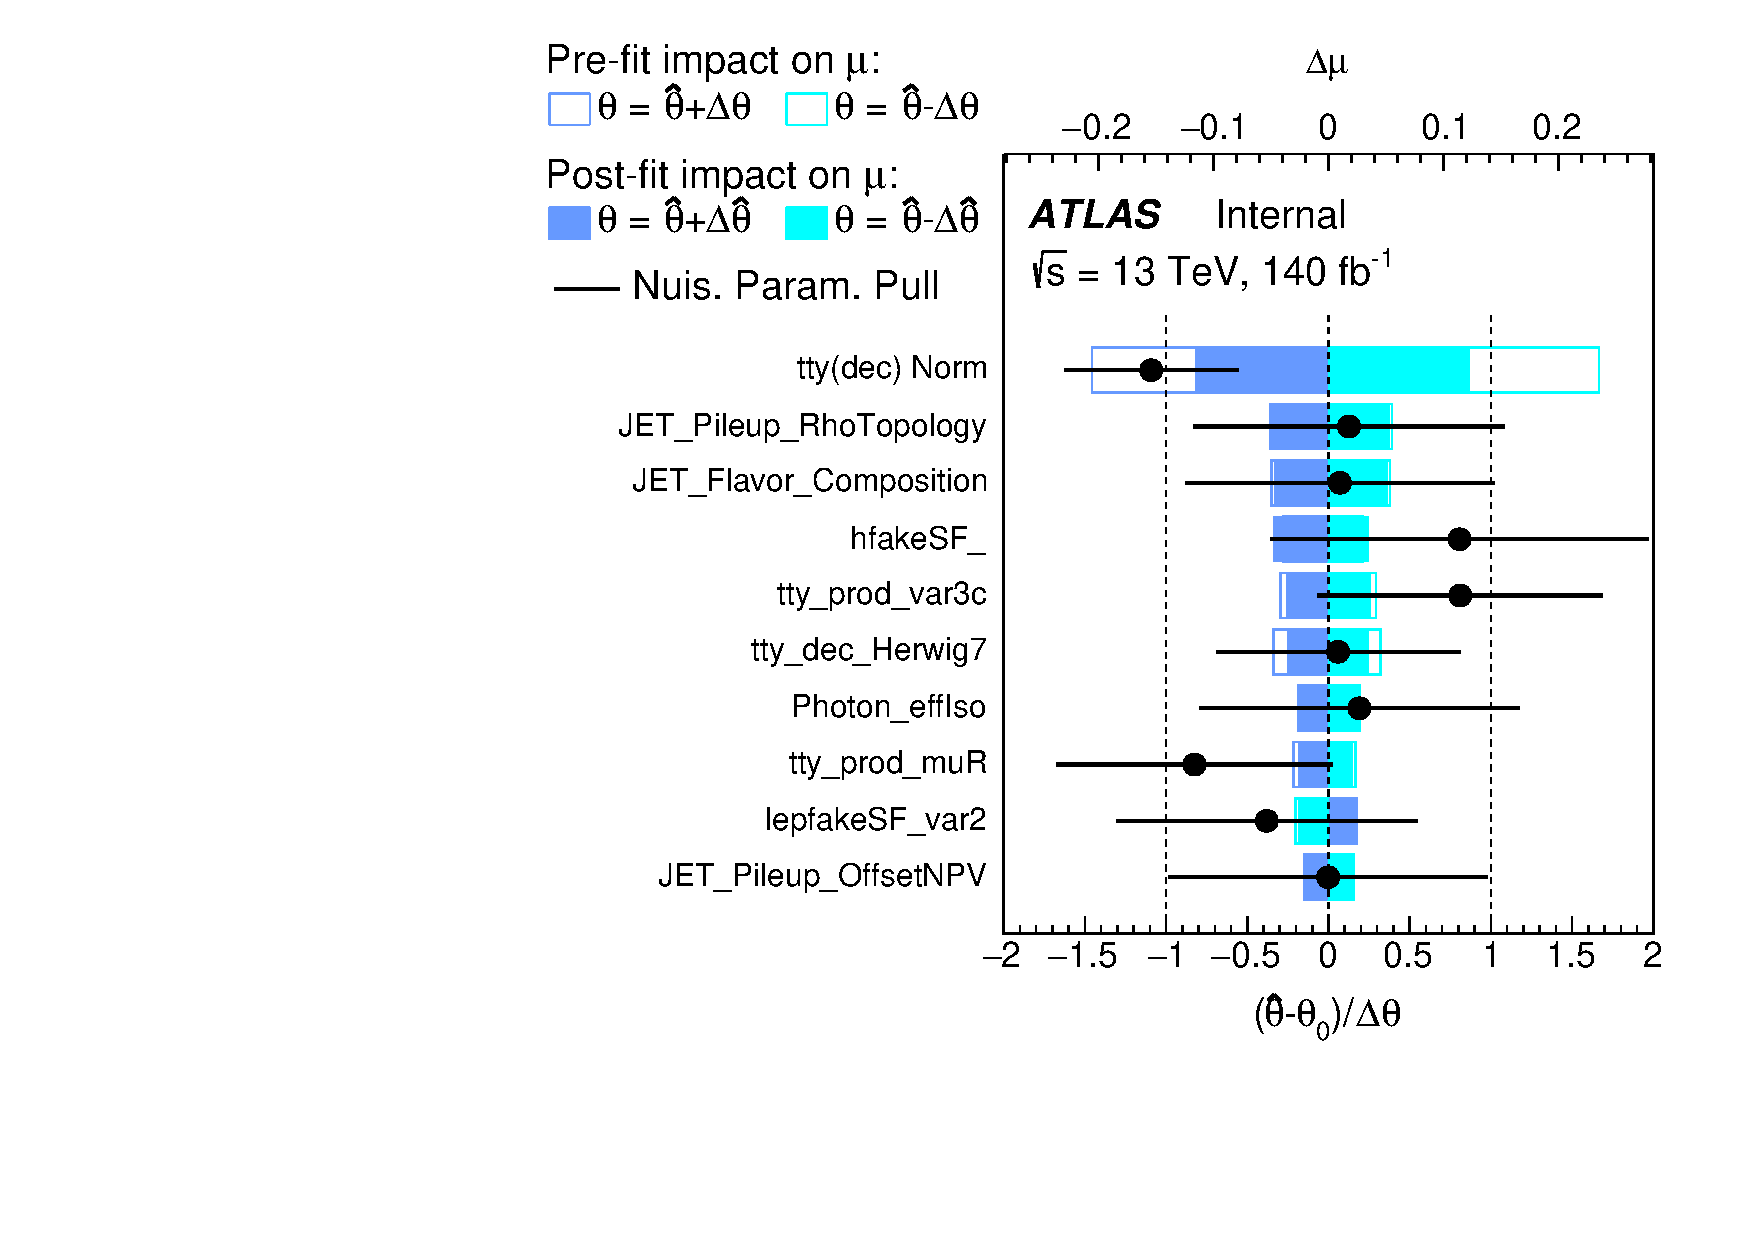
\includegraphics[width=0.2\textwidth]{figures/diff_xsec/ljet_tty_total_mu_blinded/Ranking/tty1l_pt_all_syst/Ranking_tty_pt_Bin_001_mu.pdf}}
  \quad
  \subfloat[]{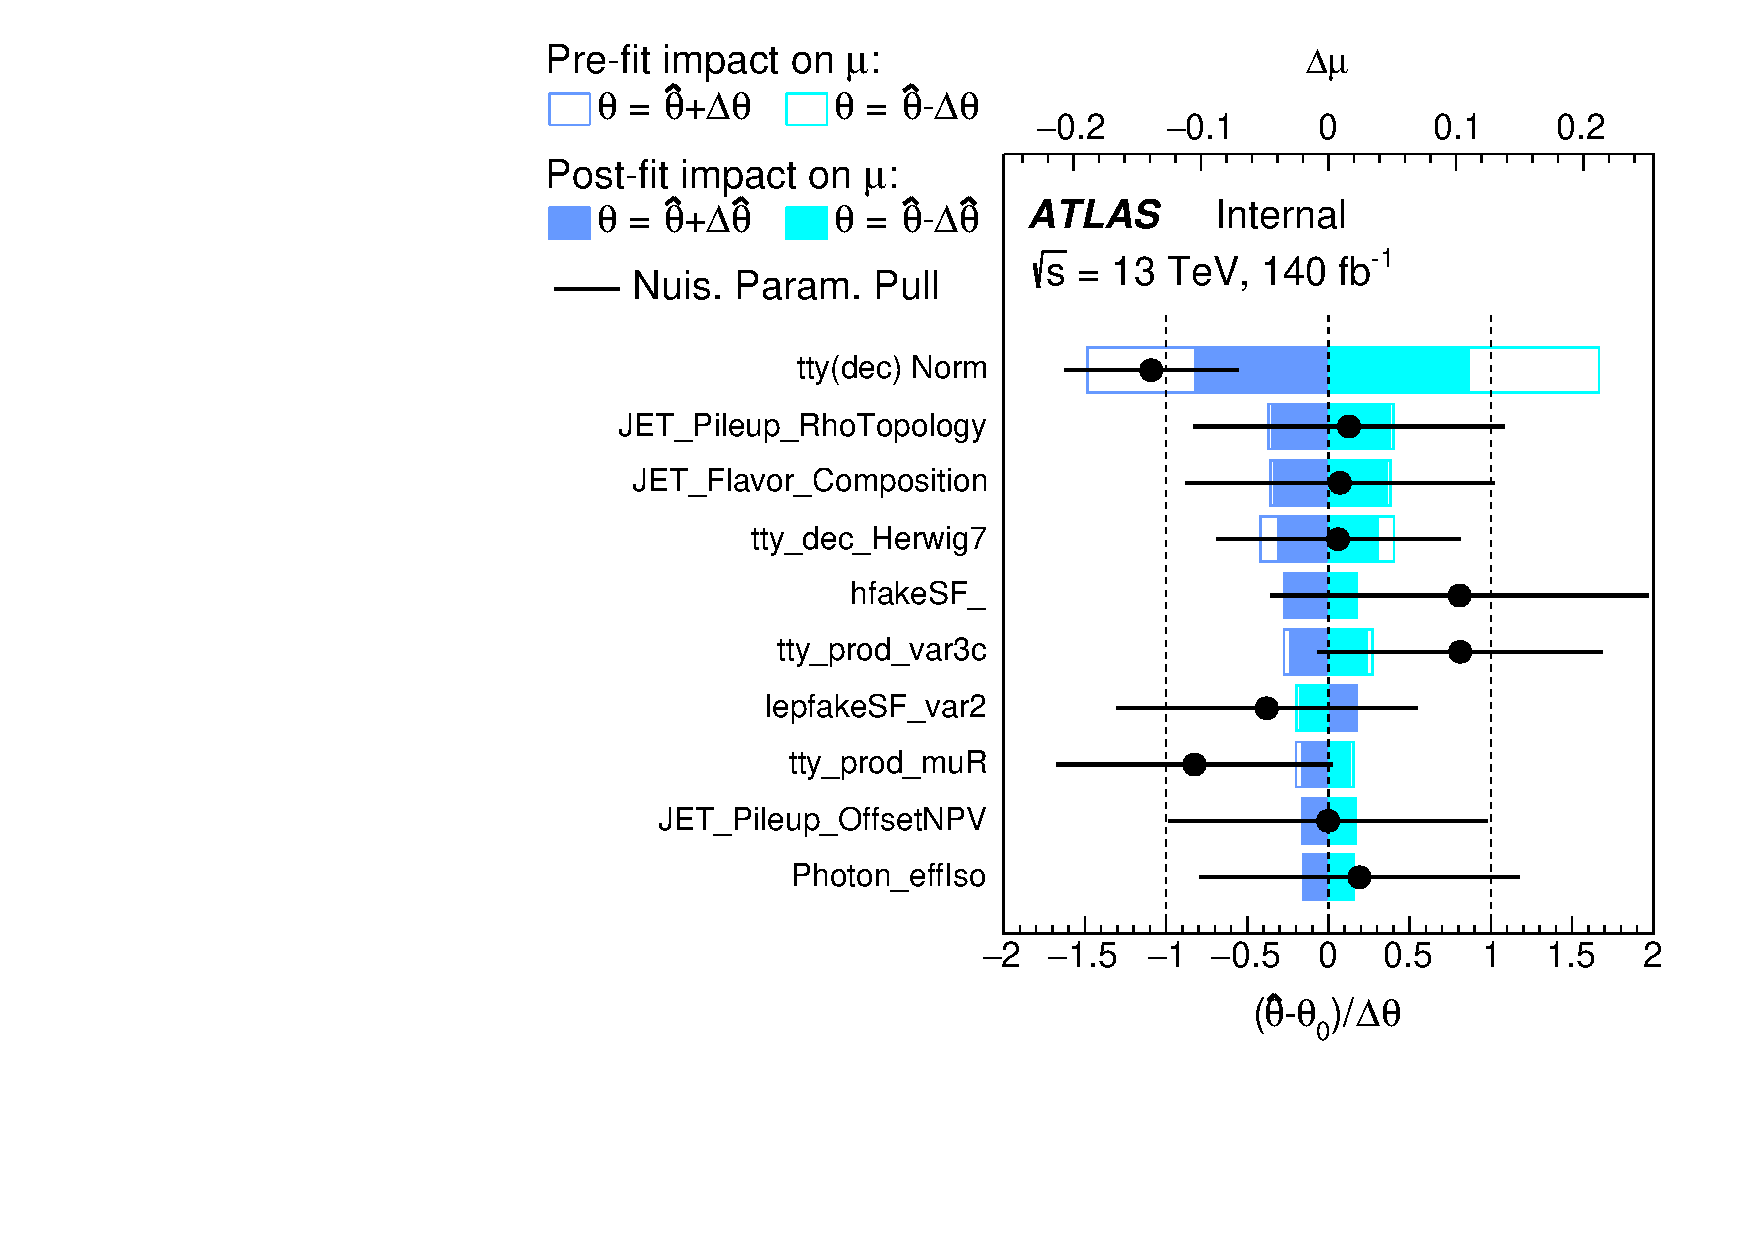
\includegraphics[width=0.2\textwidth]{figures/diff_xsec/ljet_tty_total_mu_blinded/Ranking/tty1l_pt_all_syst/Ranking_tty_pt_Bin_002_mu.pdf}}
  \quad
  \subfloat[]{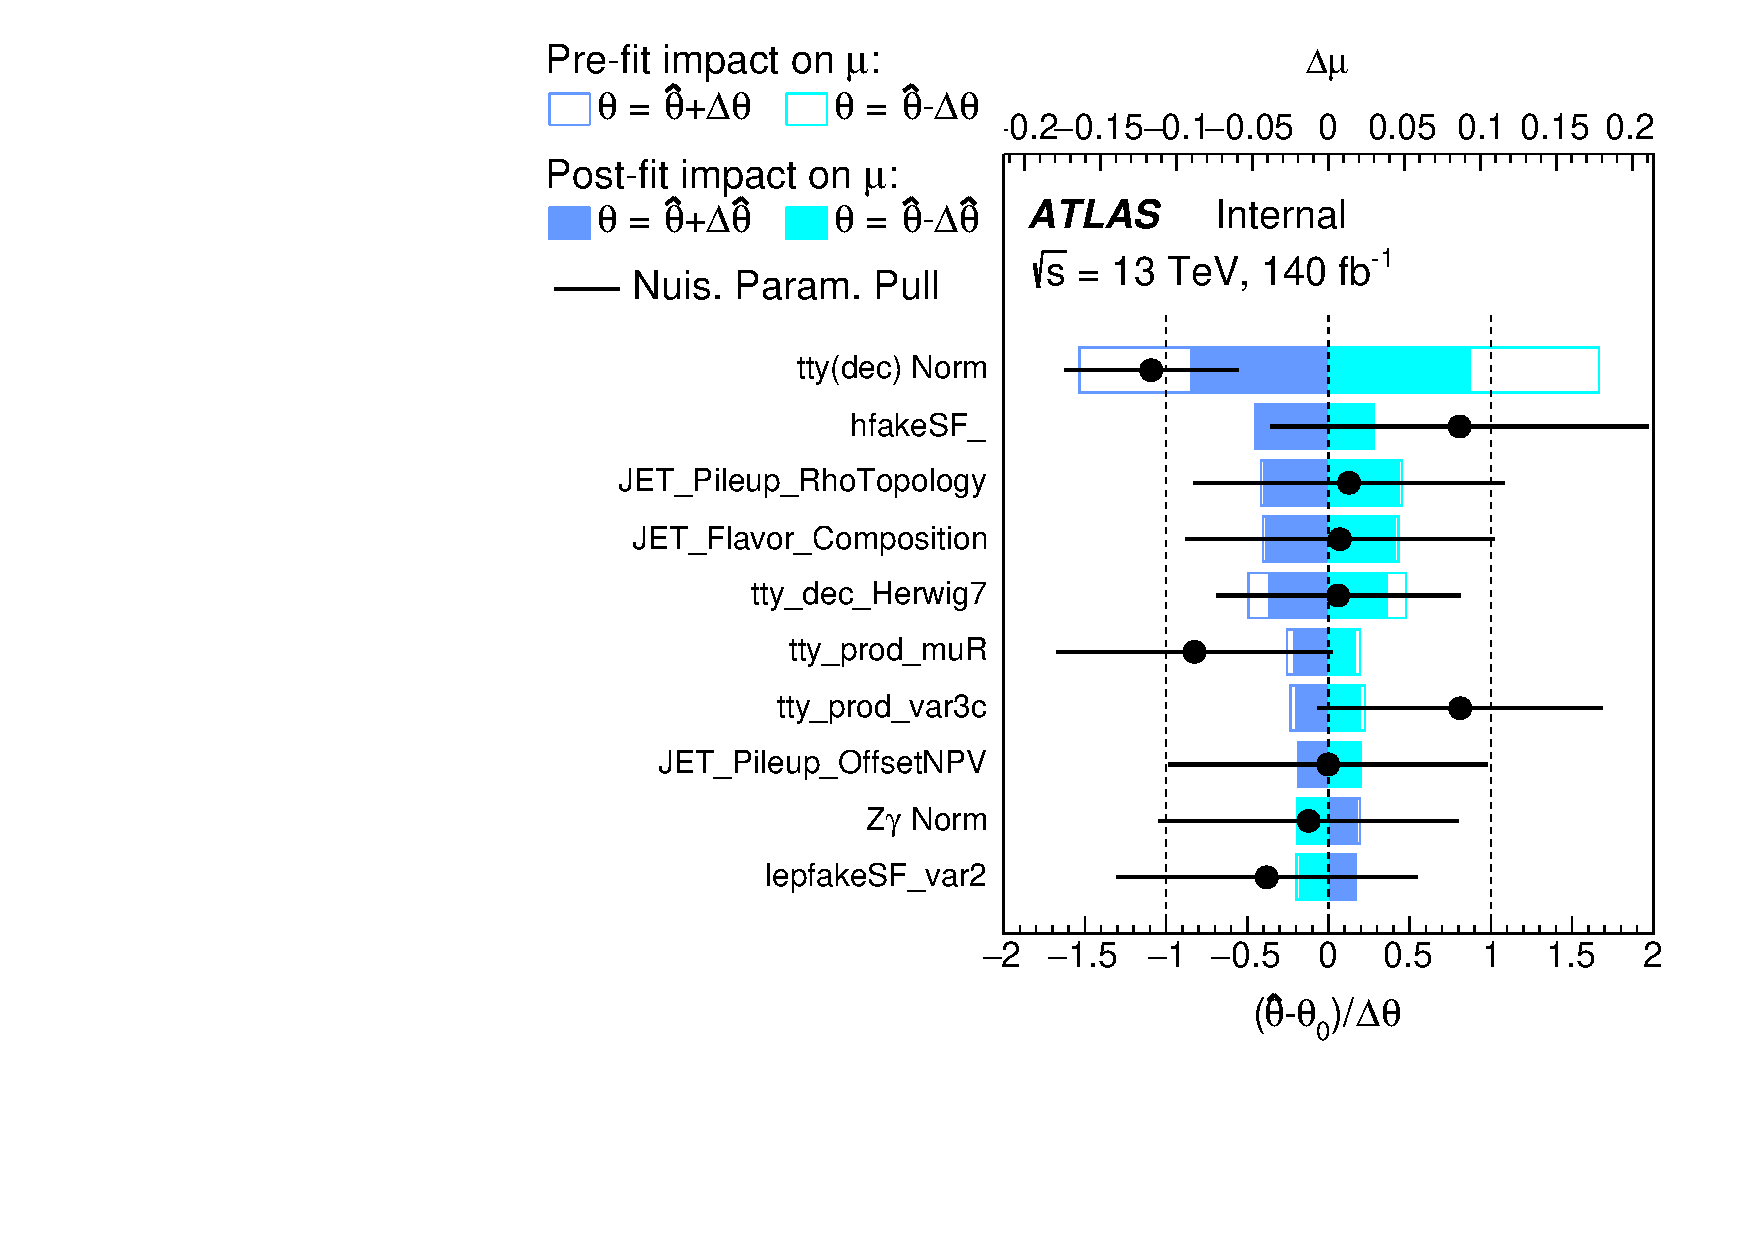
\includegraphics[width=0.2\textwidth]{figures/diff_xsec/ljet_tty_total_mu_blinded/Ranking/tty1l_pt_all_syst/Ranking_tty_pt_Bin_003_mu.pdf}}
  \quad
  \subfloat[]{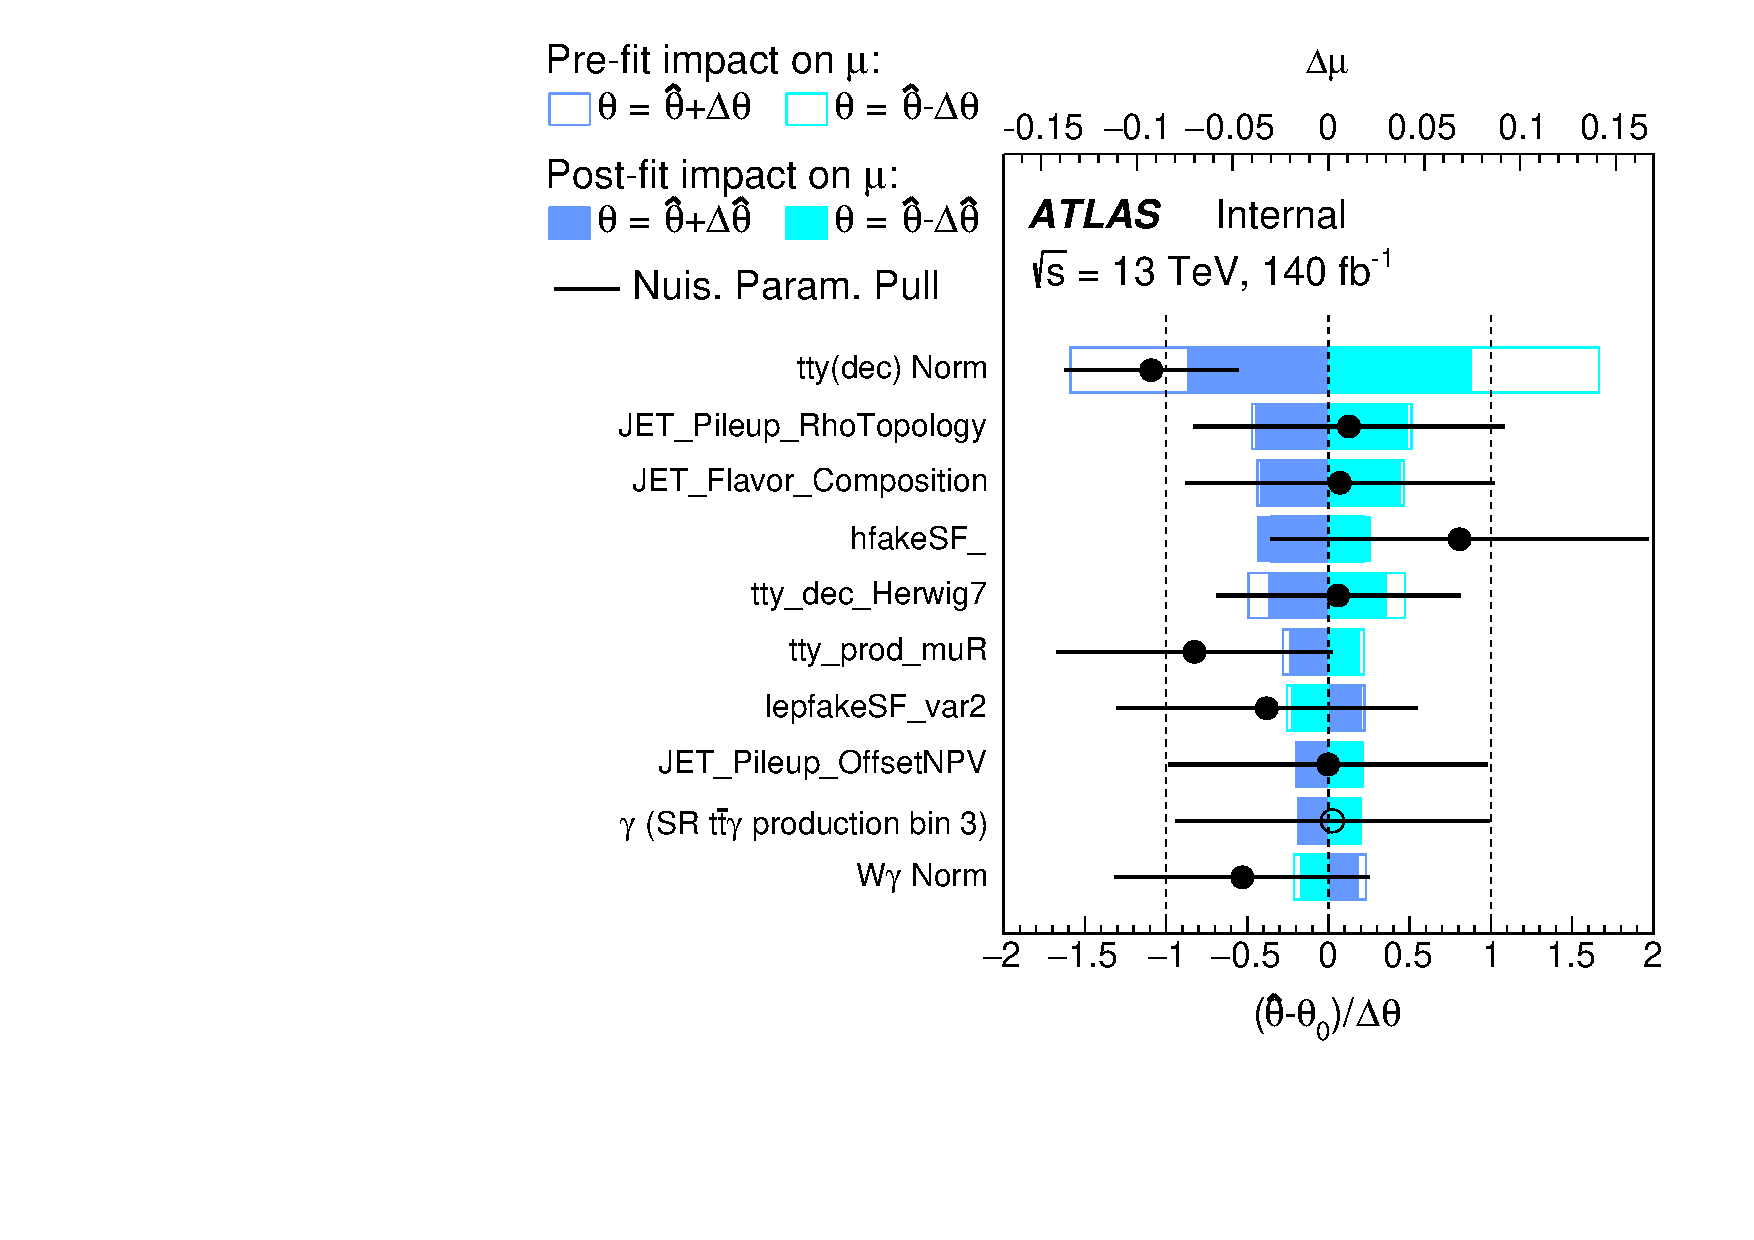
\includegraphics[width=0.2\textwidth]{figures/diff_xsec/ljet_tty_total_mu_blinded/Ranking/tty1l_pt_all_syst/Ranking_tty_pt_Bin_004_mu.pdf}}
  \quad
  \subfloat[]{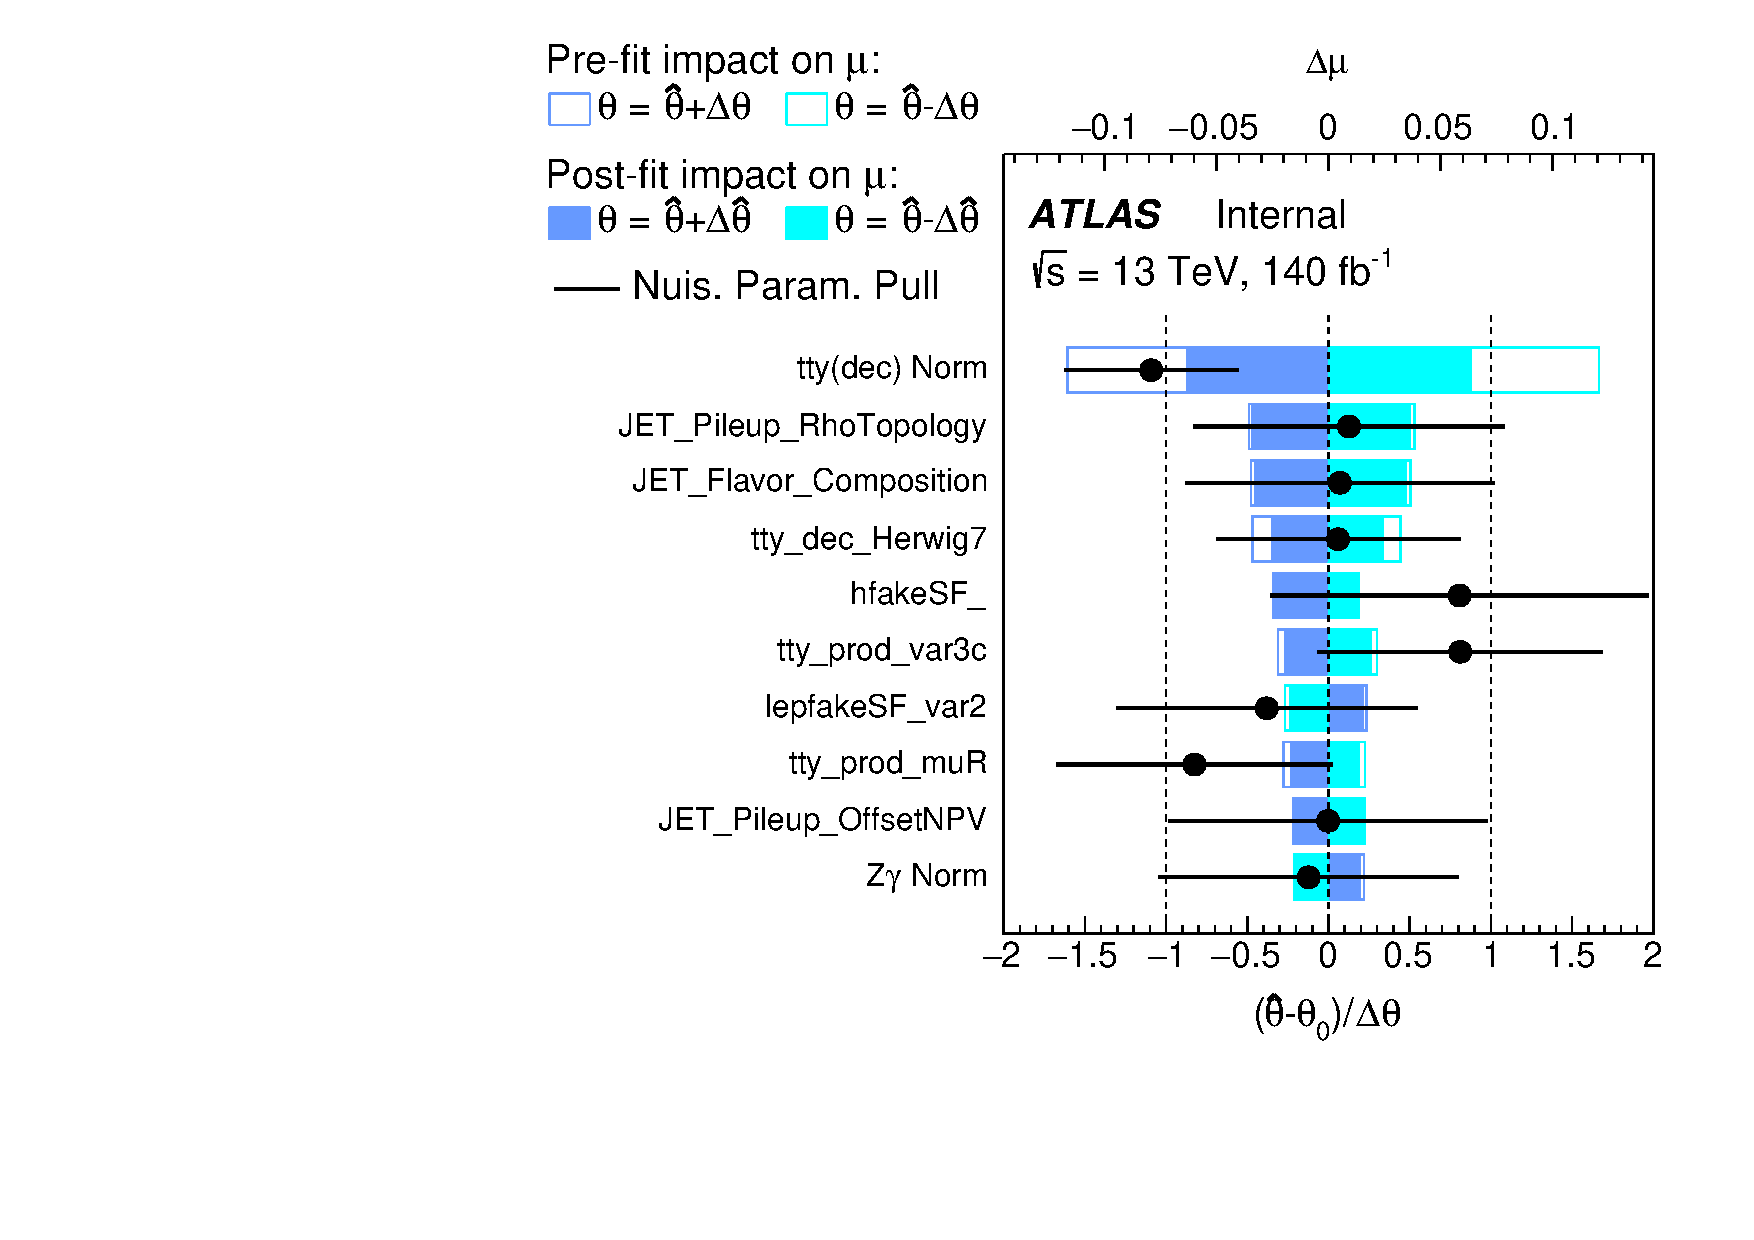
\includegraphics[width=0.2\textwidth]{figures/diff_xsec/ljet_tty_total_mu_blinded/Ranking/tty1l_pt_all_syst/Ranking_tty_pt_Bin_005_mu.pdf}}
  \quad
  \subfloat[]{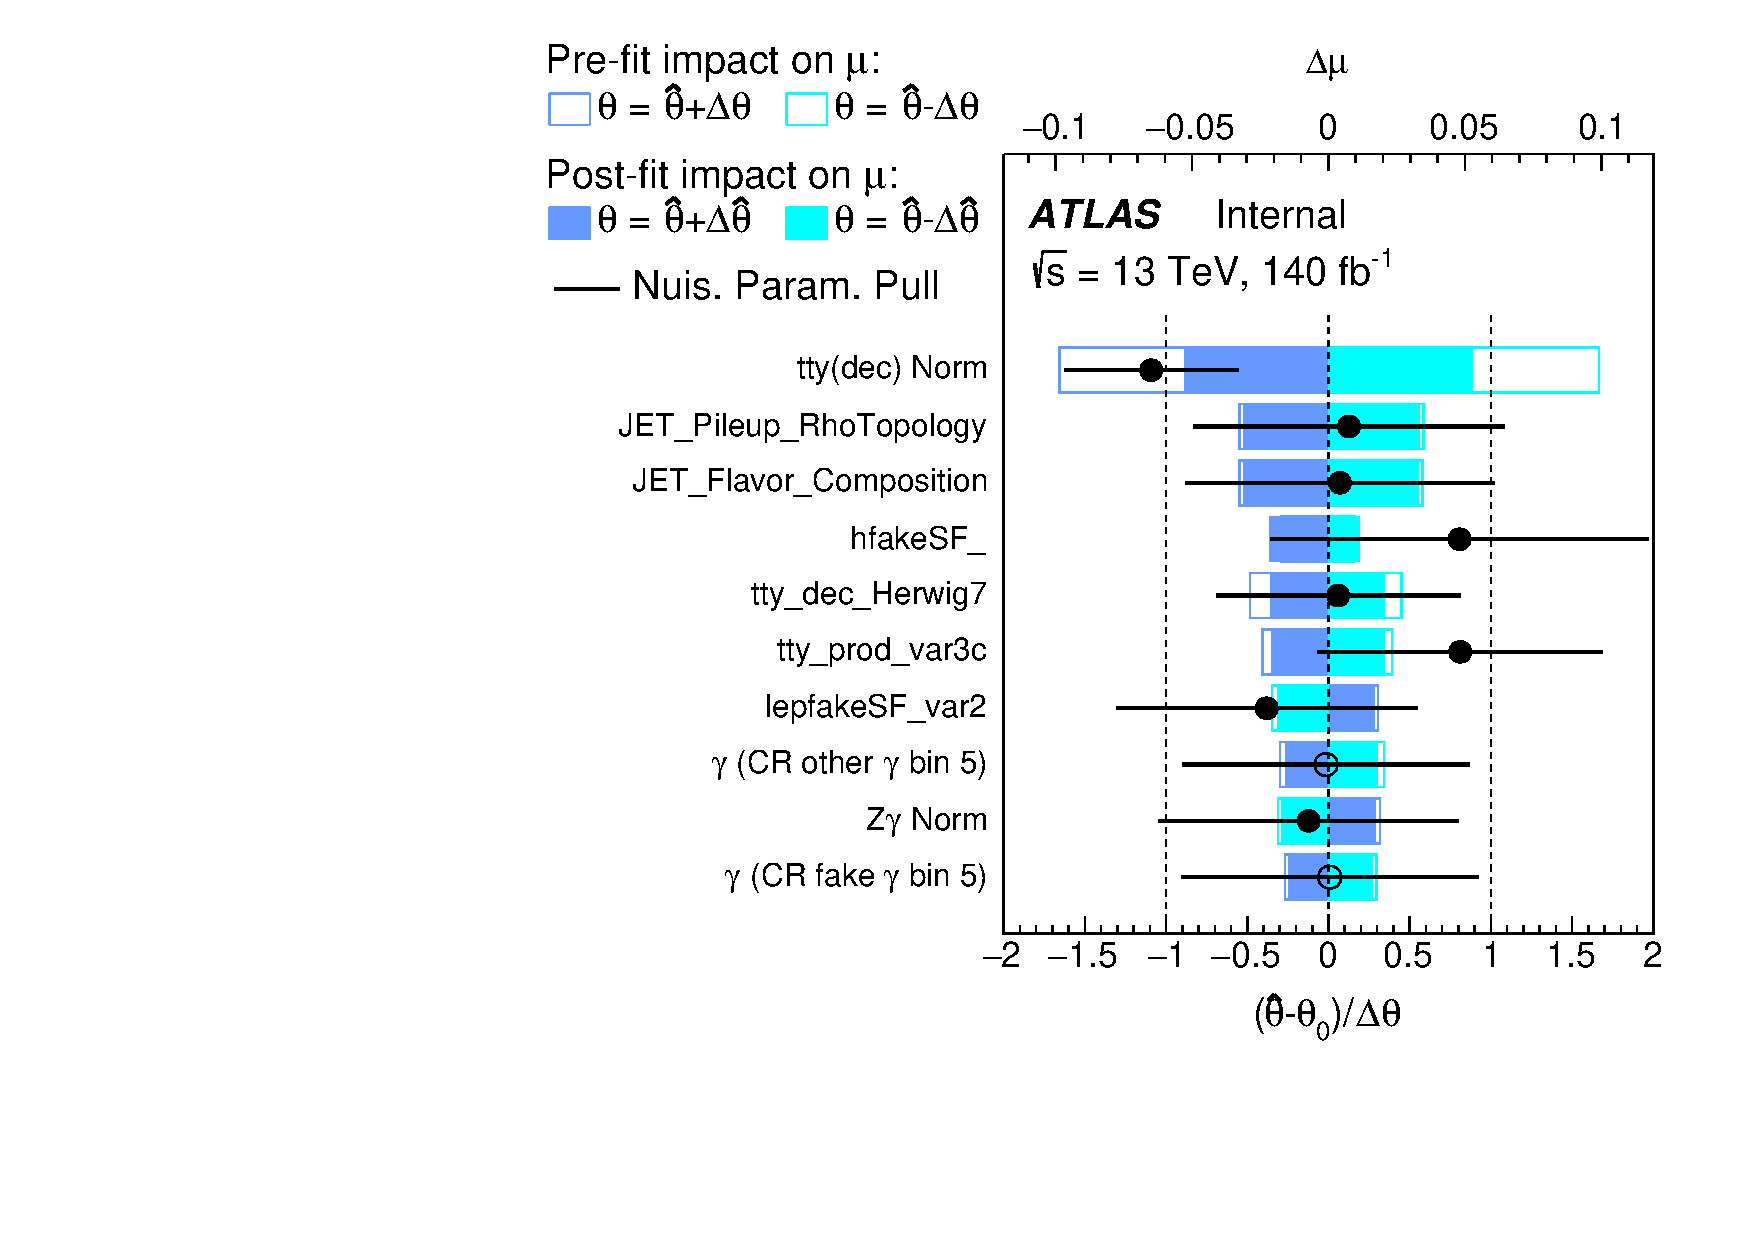
\includegraphics[width=0.2\textwidth]{figures/diff_xsec/ljet_tty_total_mu_blinded/Ranking/tty1l_pt_all_syst/Ranking_tty_pt_Bin_006_mu.pdf}}
  \quad
  \subfloat[]{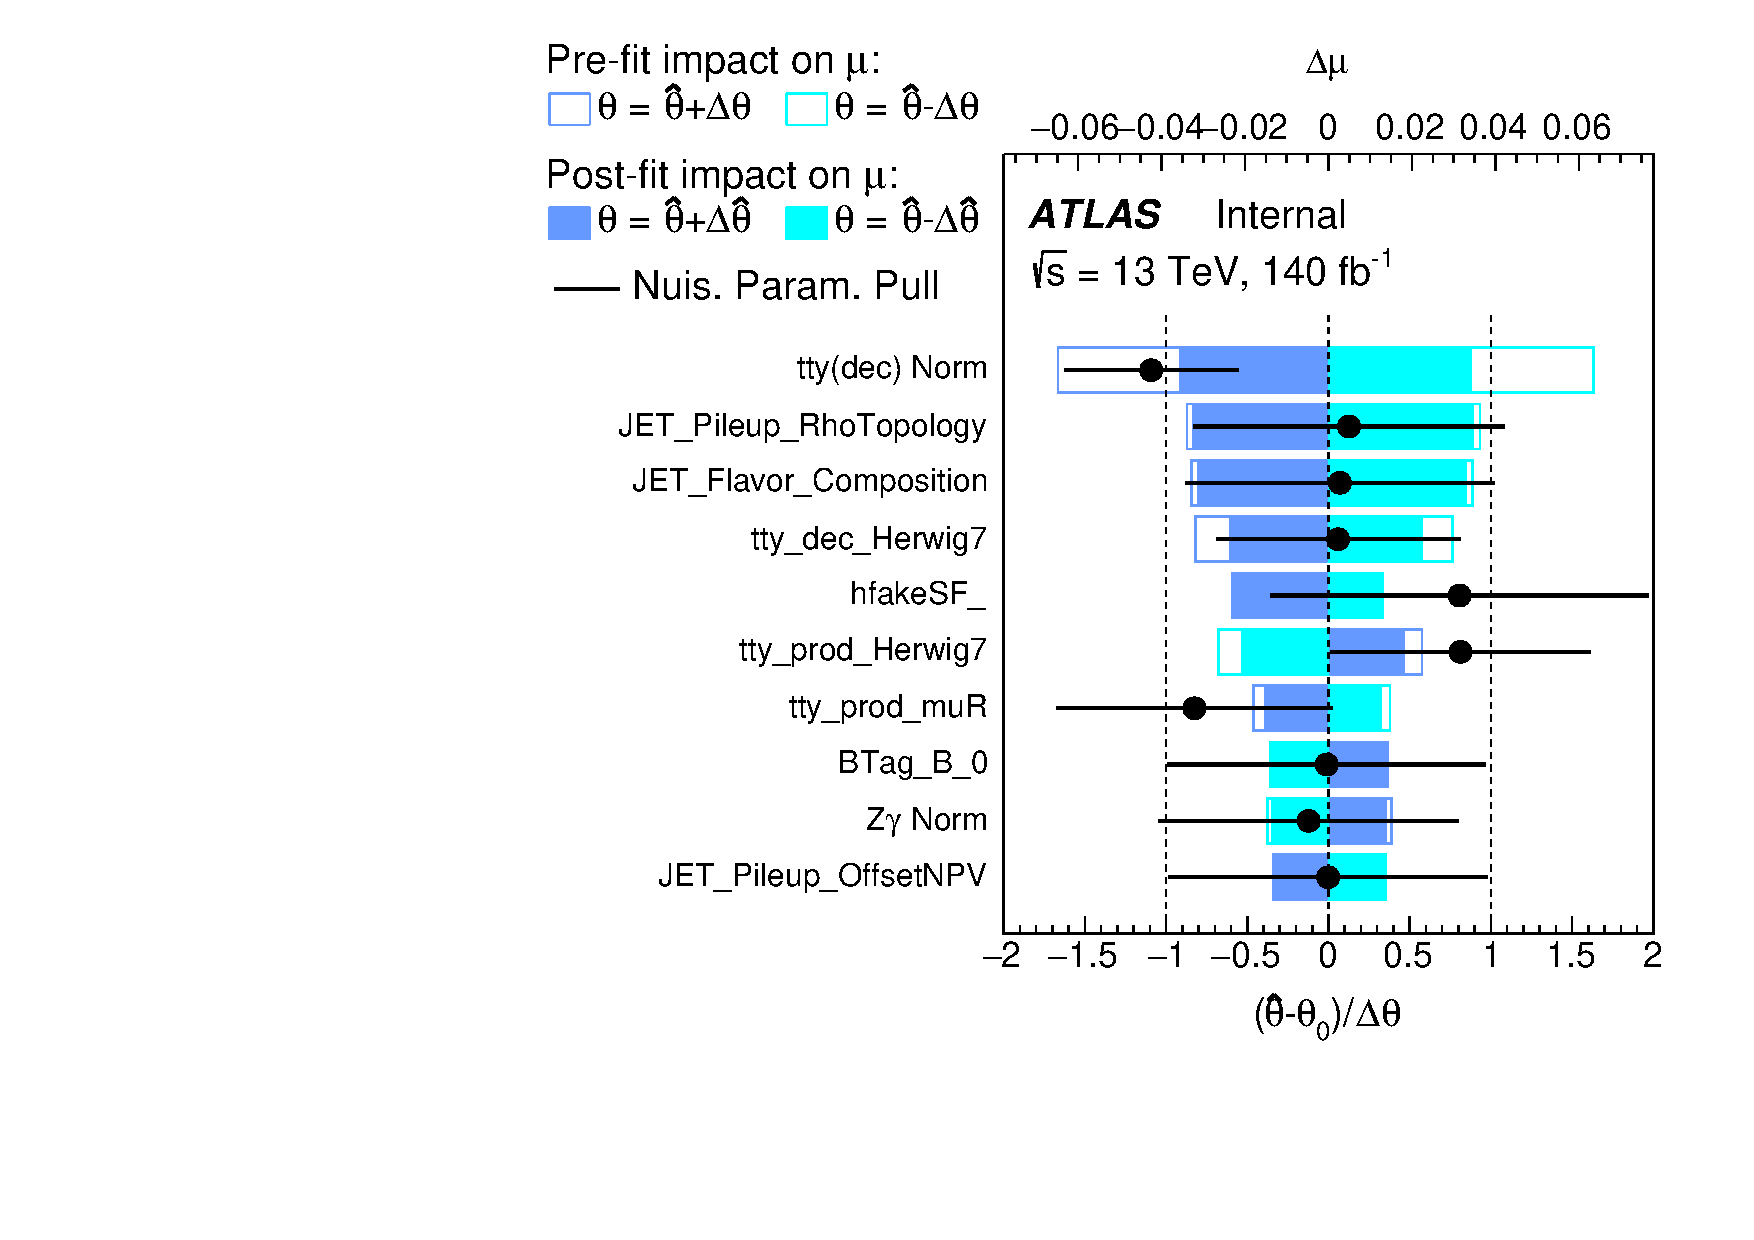
\includegraphics[width=0.2\textwidth]{figures/diff_xsec/ljet_tty_total_mu_blinded/Ranking/tty1l_pt_all_syst/Ranking_tty_pt_Bin_007_mu.pdf}}
  \quad
  \subfloat[]{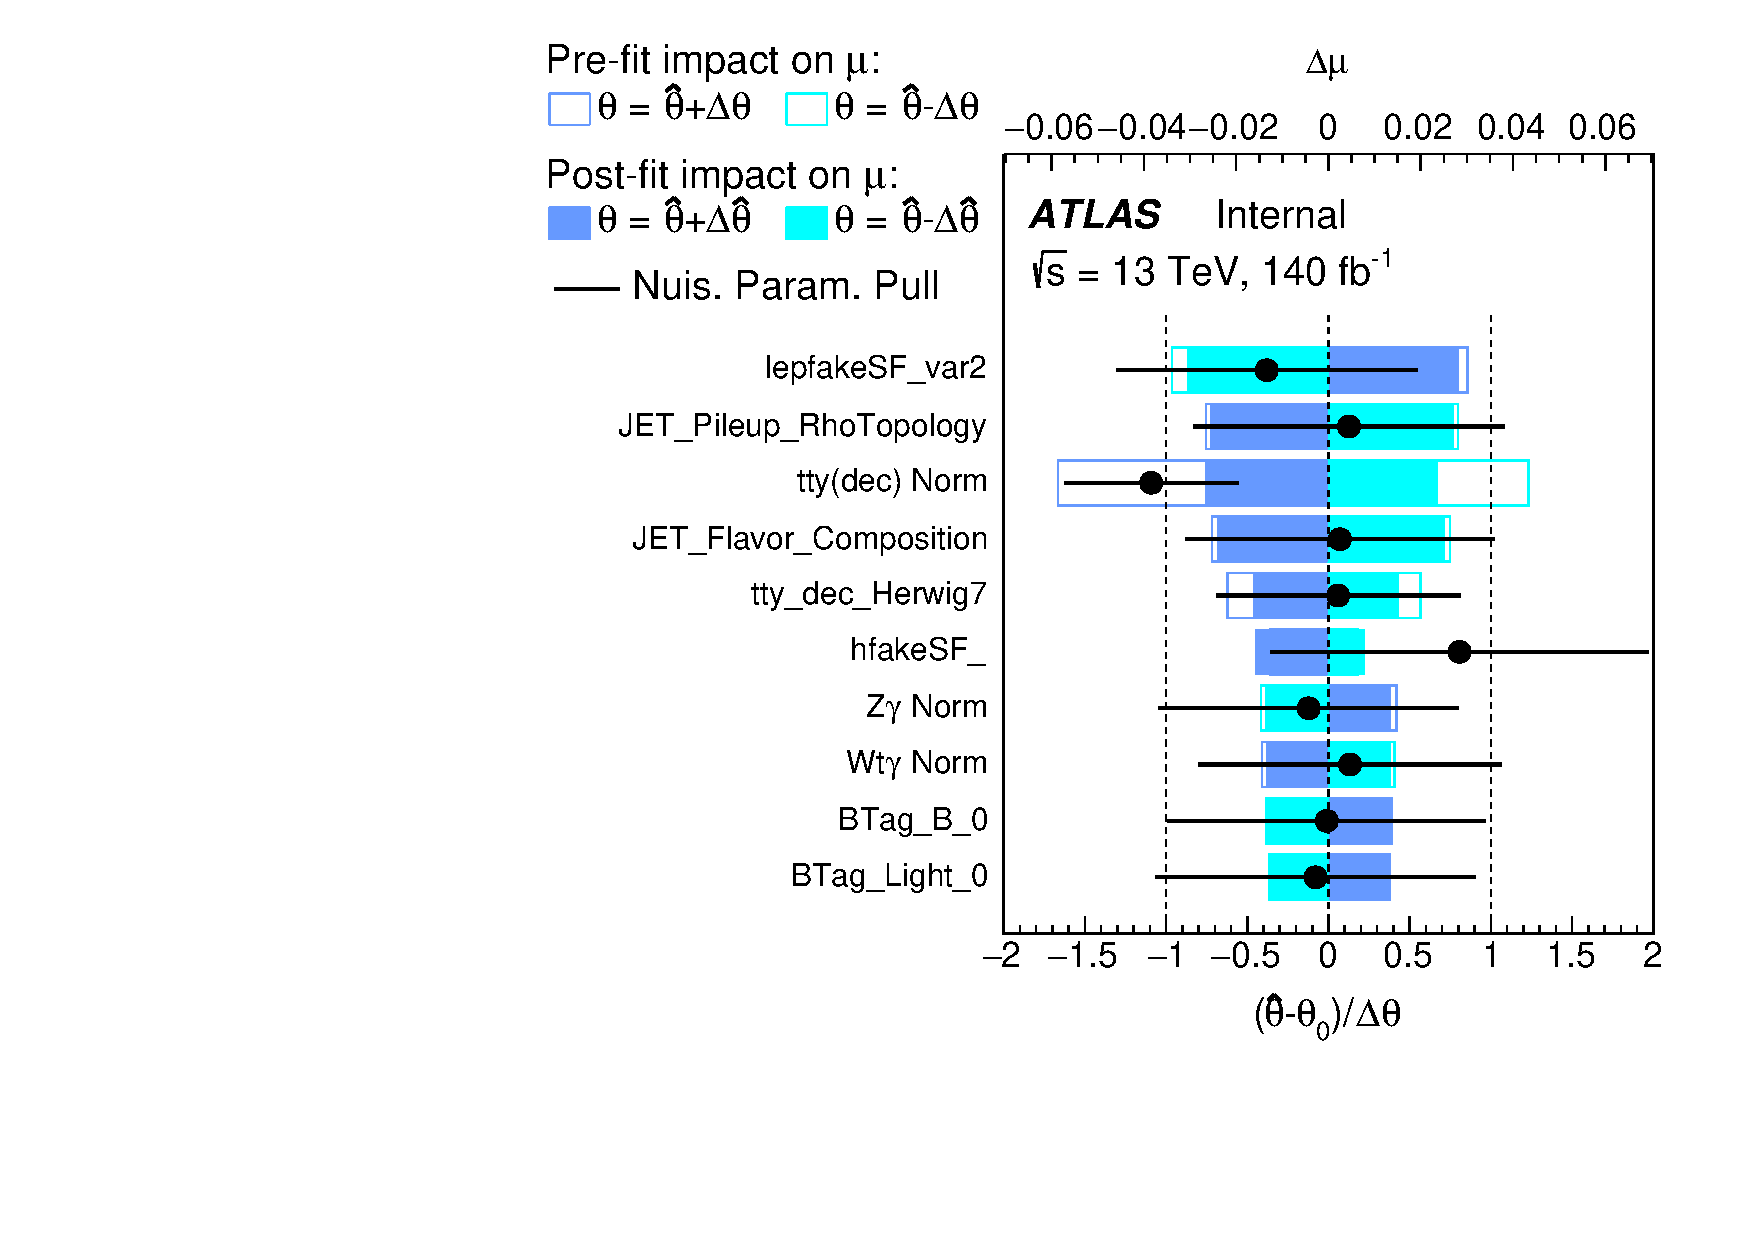
\includegraphics[width=0.2\textwidth]{figures/diff_xsec/ljet_tty_total_mu_blinded/Ranking/tty1l_pt_all_syst/Ranking_tty_pt_Bin_008_mu.pdf}}
  \quad
  \subfloat[]{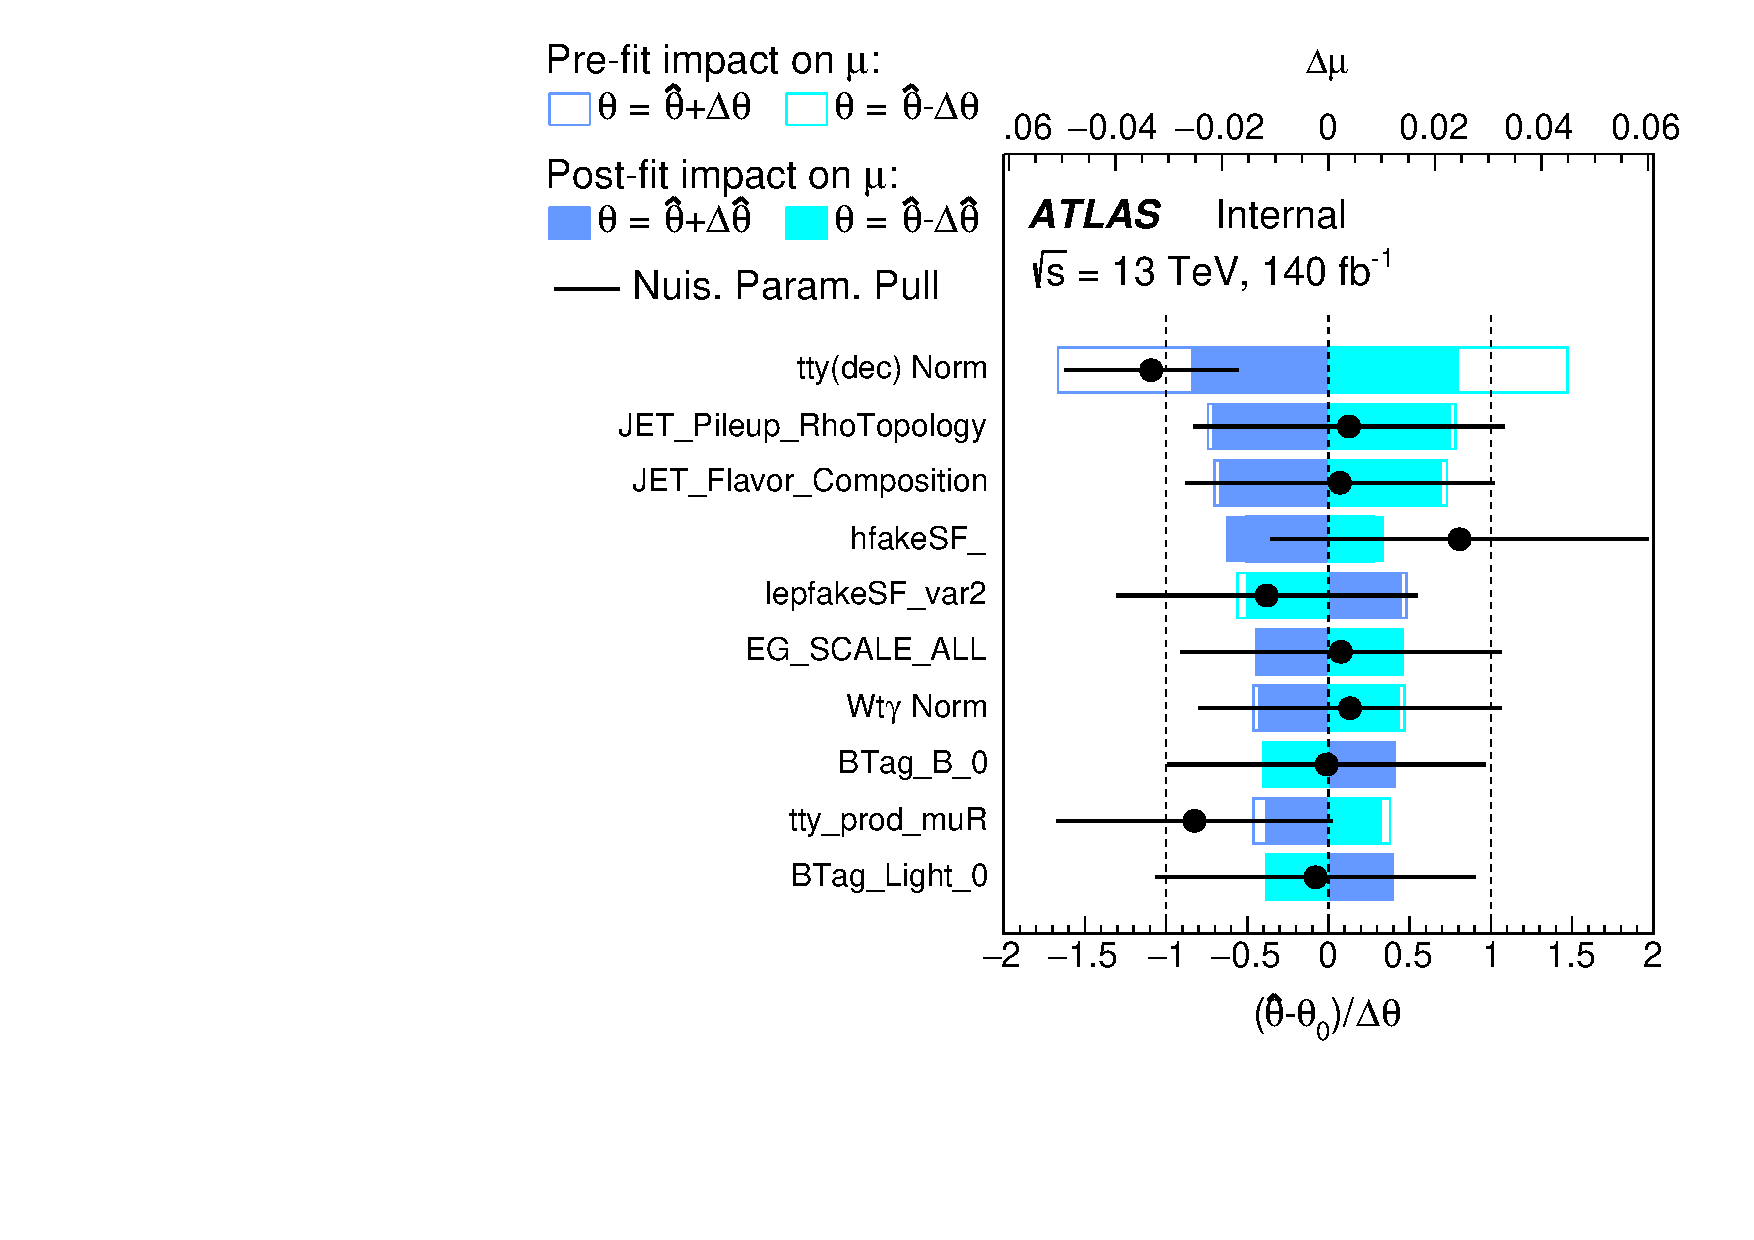
\includegraphics[width=0.2\textwidth]{figures/diff_xsec/ljet_tty_total_mu_blinded/Ranking/tty1l_pt_all_syst/Ranking_tty_pt_Bin_009_mu.pdf}}
  \quad
  \subfloat[]{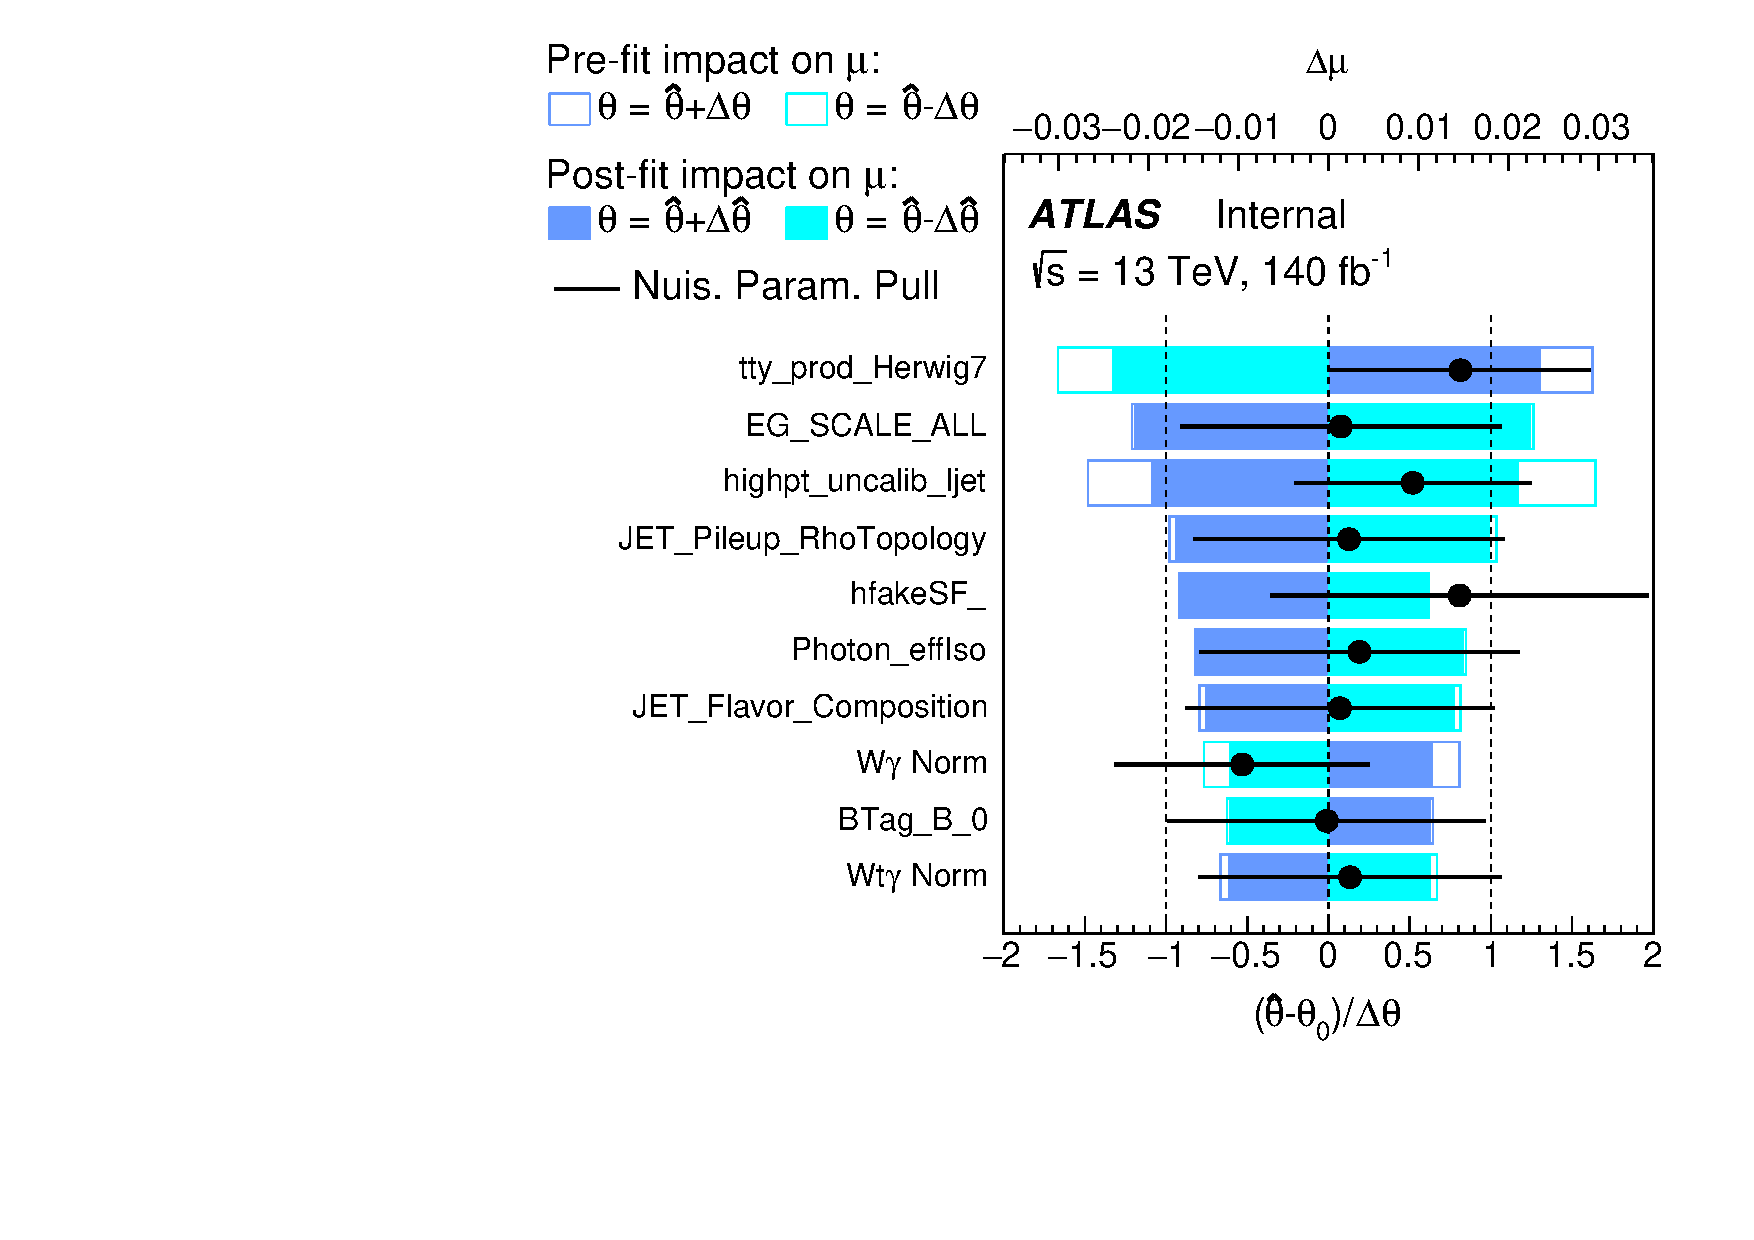
\includegraphics[width=0.2\textwidth]{figures/diff_xsec/ljet_tty_total_mu_blinded/Ranking/tty1l_pt_all_syst/Ranking_tty_pt_Bin_010_mu.pdf}}

  \caption{Ranking plots of the 10 NPs with the largest impact on the \tty (total) singal strength in each bin of the $p_T(\gamma)$ distribution in the single 
  lepton channel. The fit was performed to the data keeping the POIs blinded. Each subfigure, labeled (a), (b), (c), (d)... (j), corresponds to a specific bin 
  of the $p_T(\gamma)$ distribution, with bin 1 represented in subfigure (a), bin 2 represented in 
  subfigure (b), and so on.}
  \label{fig:ranking_ljet_total_mu_blinded}
\end{figure}
\FloatBarrier


\begin{figure}[ht]
  \centering
  \subfloat[]{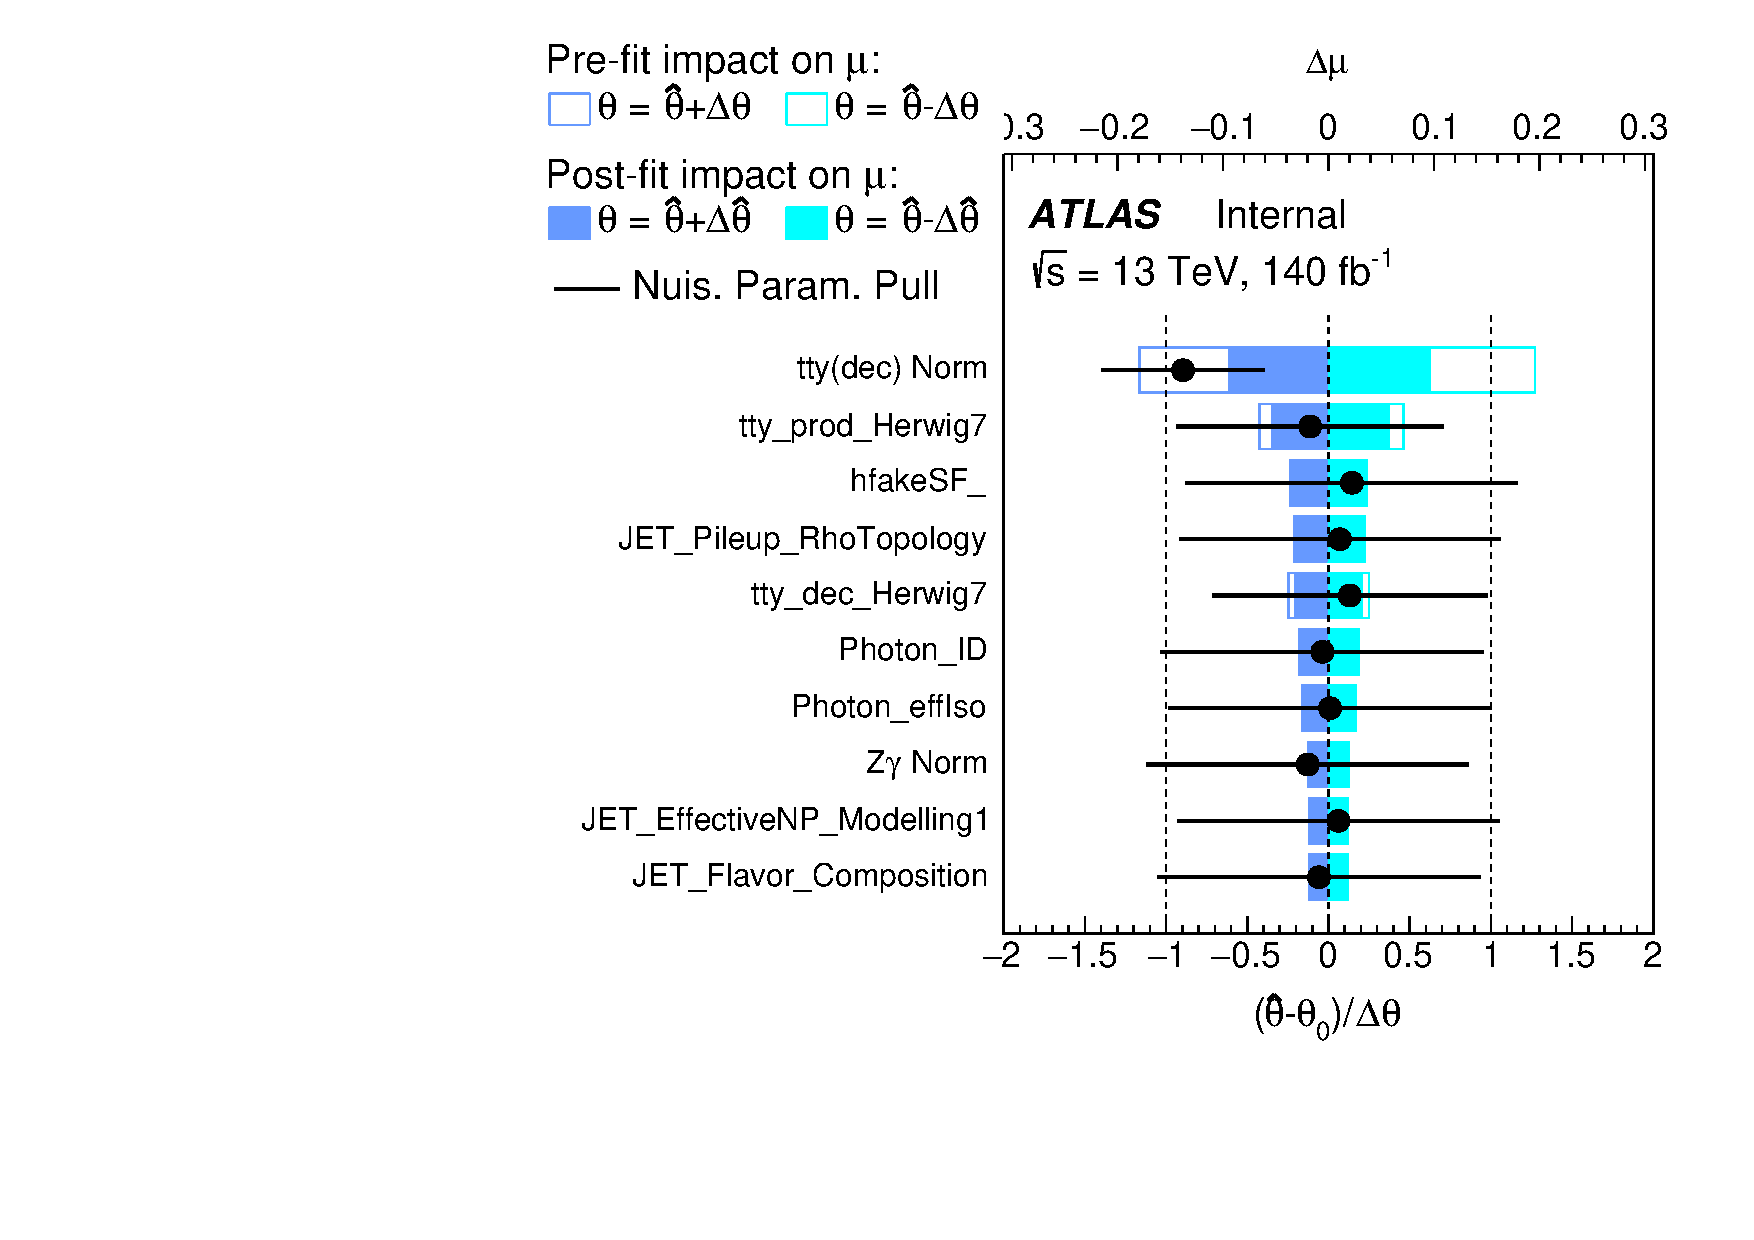
\includegraphics[width=0.2\textwidth]{figures/diff_xsec/dilep_tty_total_mu_blinded/Ranking/tty2l_pt_all_syst/Ranking_tty2l_pt_all_syst_Bin_001_mu.pdf}}
  \quad
  \subfloat[]{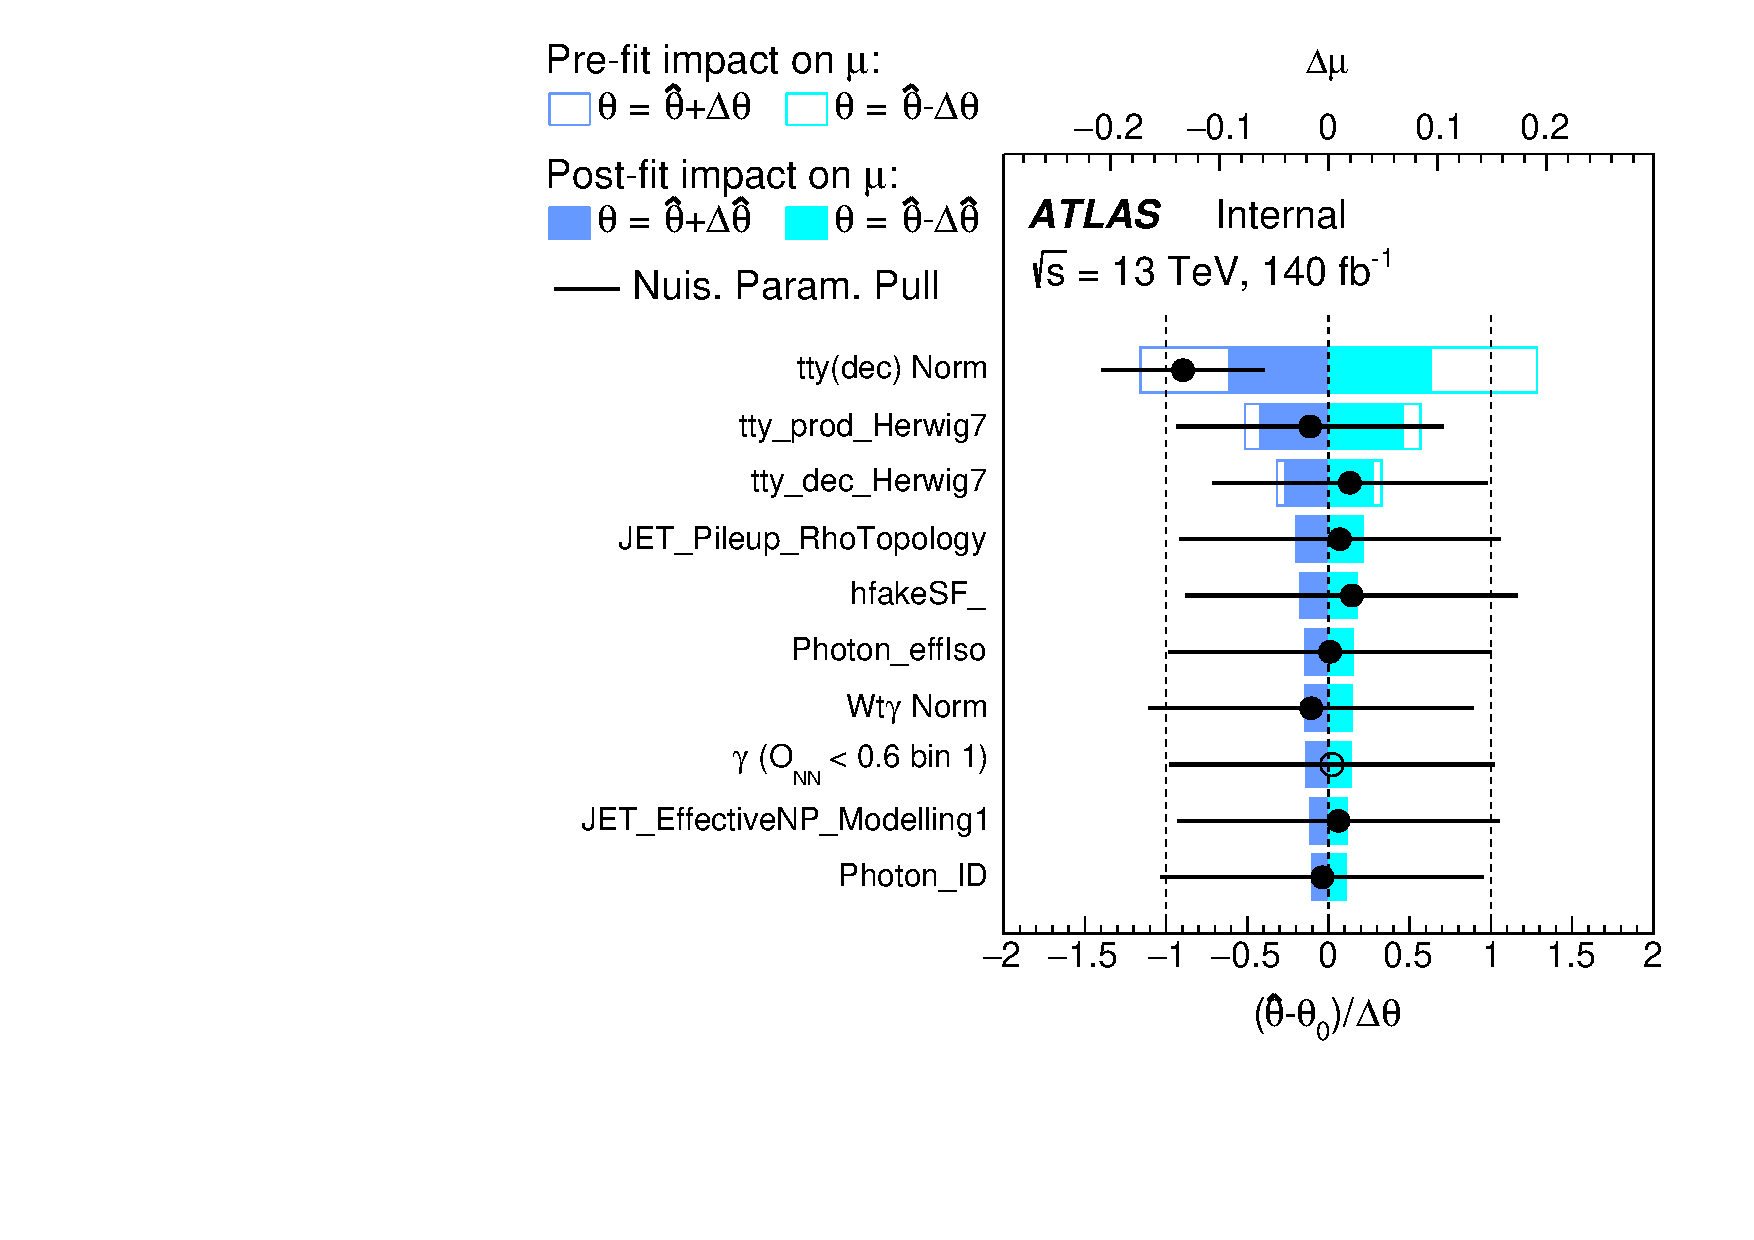
\includegraphics[width=0.2\textwidth]{figures/diff_xsec/dilep_tty_total_mu_blinded/Ranking/tty2l_pt_all_syst/Ranking_tty2l_pt_all_syst_Bin_002_mu.pdf}}
  \quad
  \subfloat[]{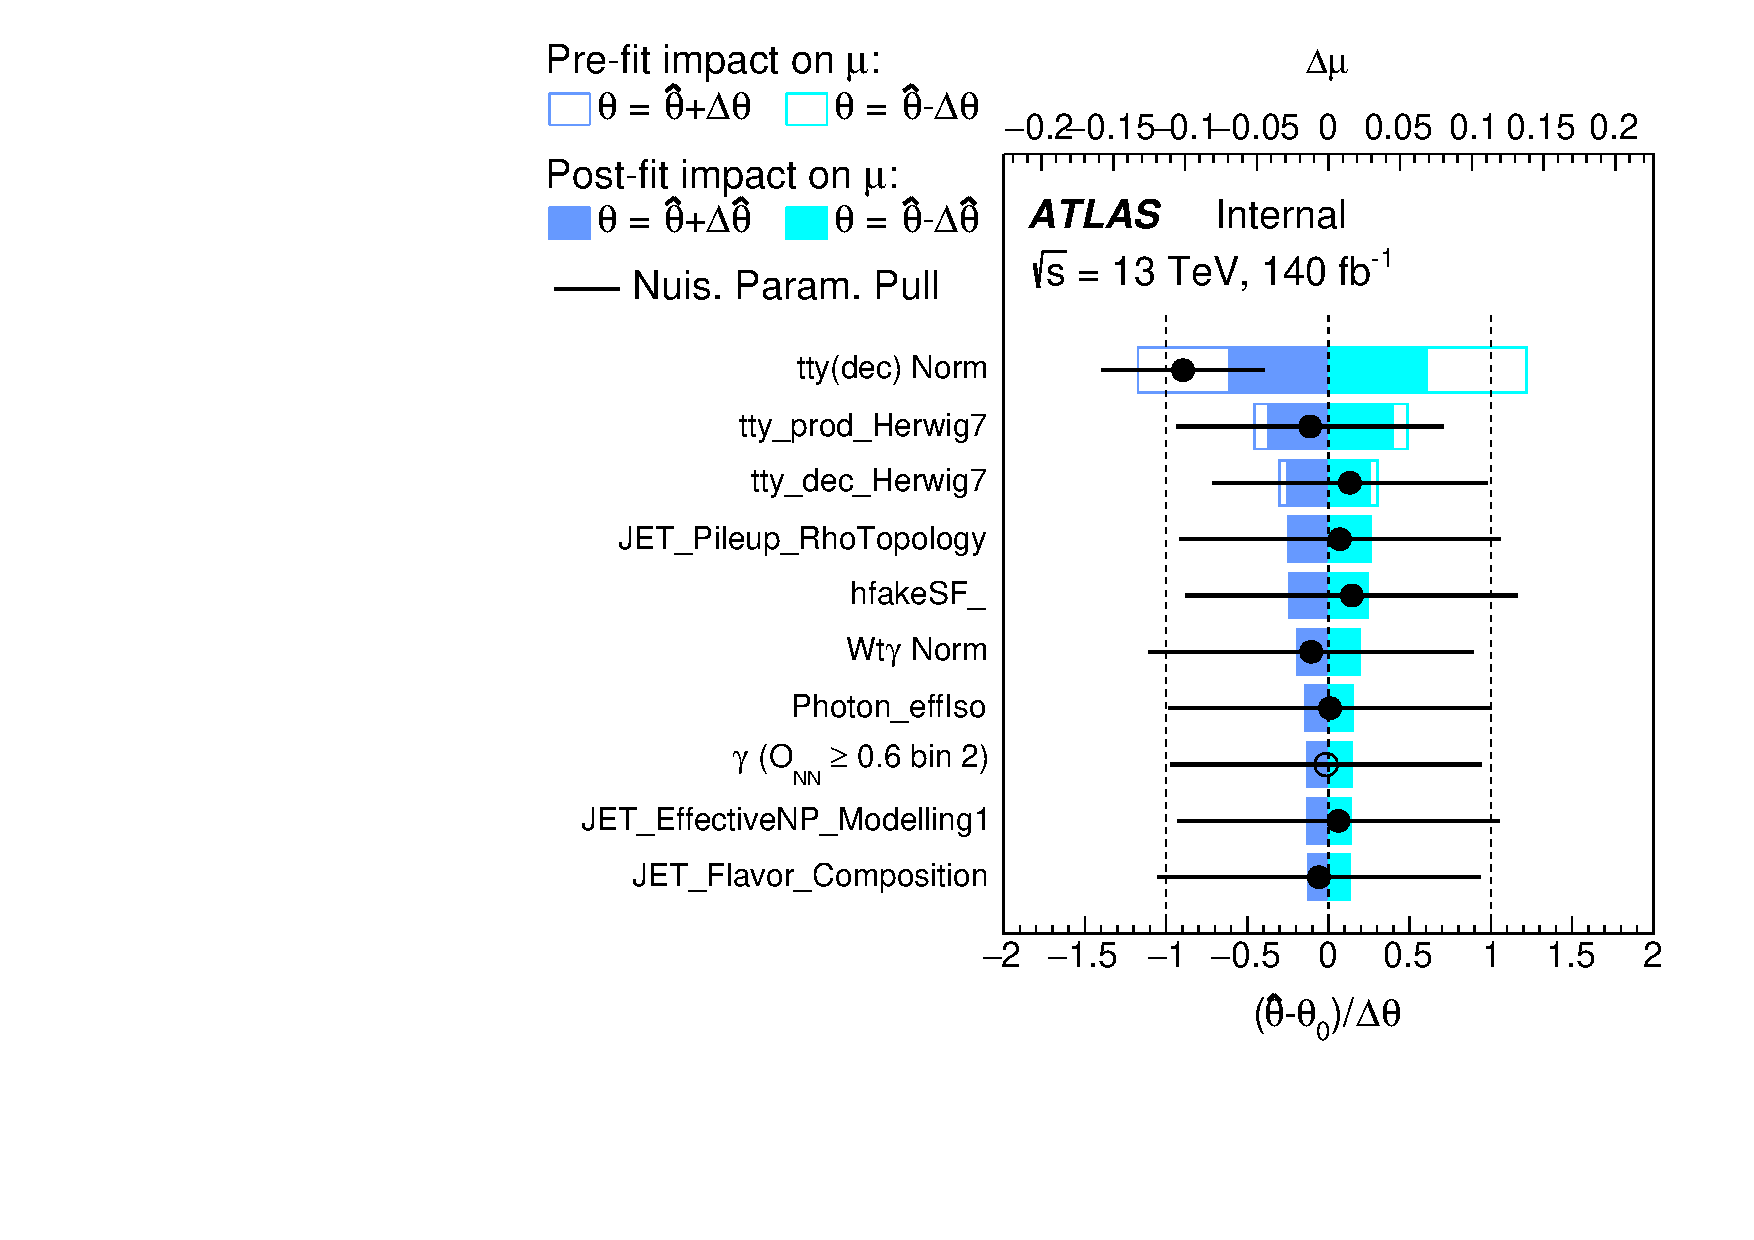
\includegraphics[width=0.2\textwidth]{figures/diff_xsec/dilep_tty_total_mu_blinded/Ranking/tty2l_pt_all_syst/Ranking_tty2l_pt_all_syst_Bin_003_mu.pdf}}
  \quad
  \subfloat[]{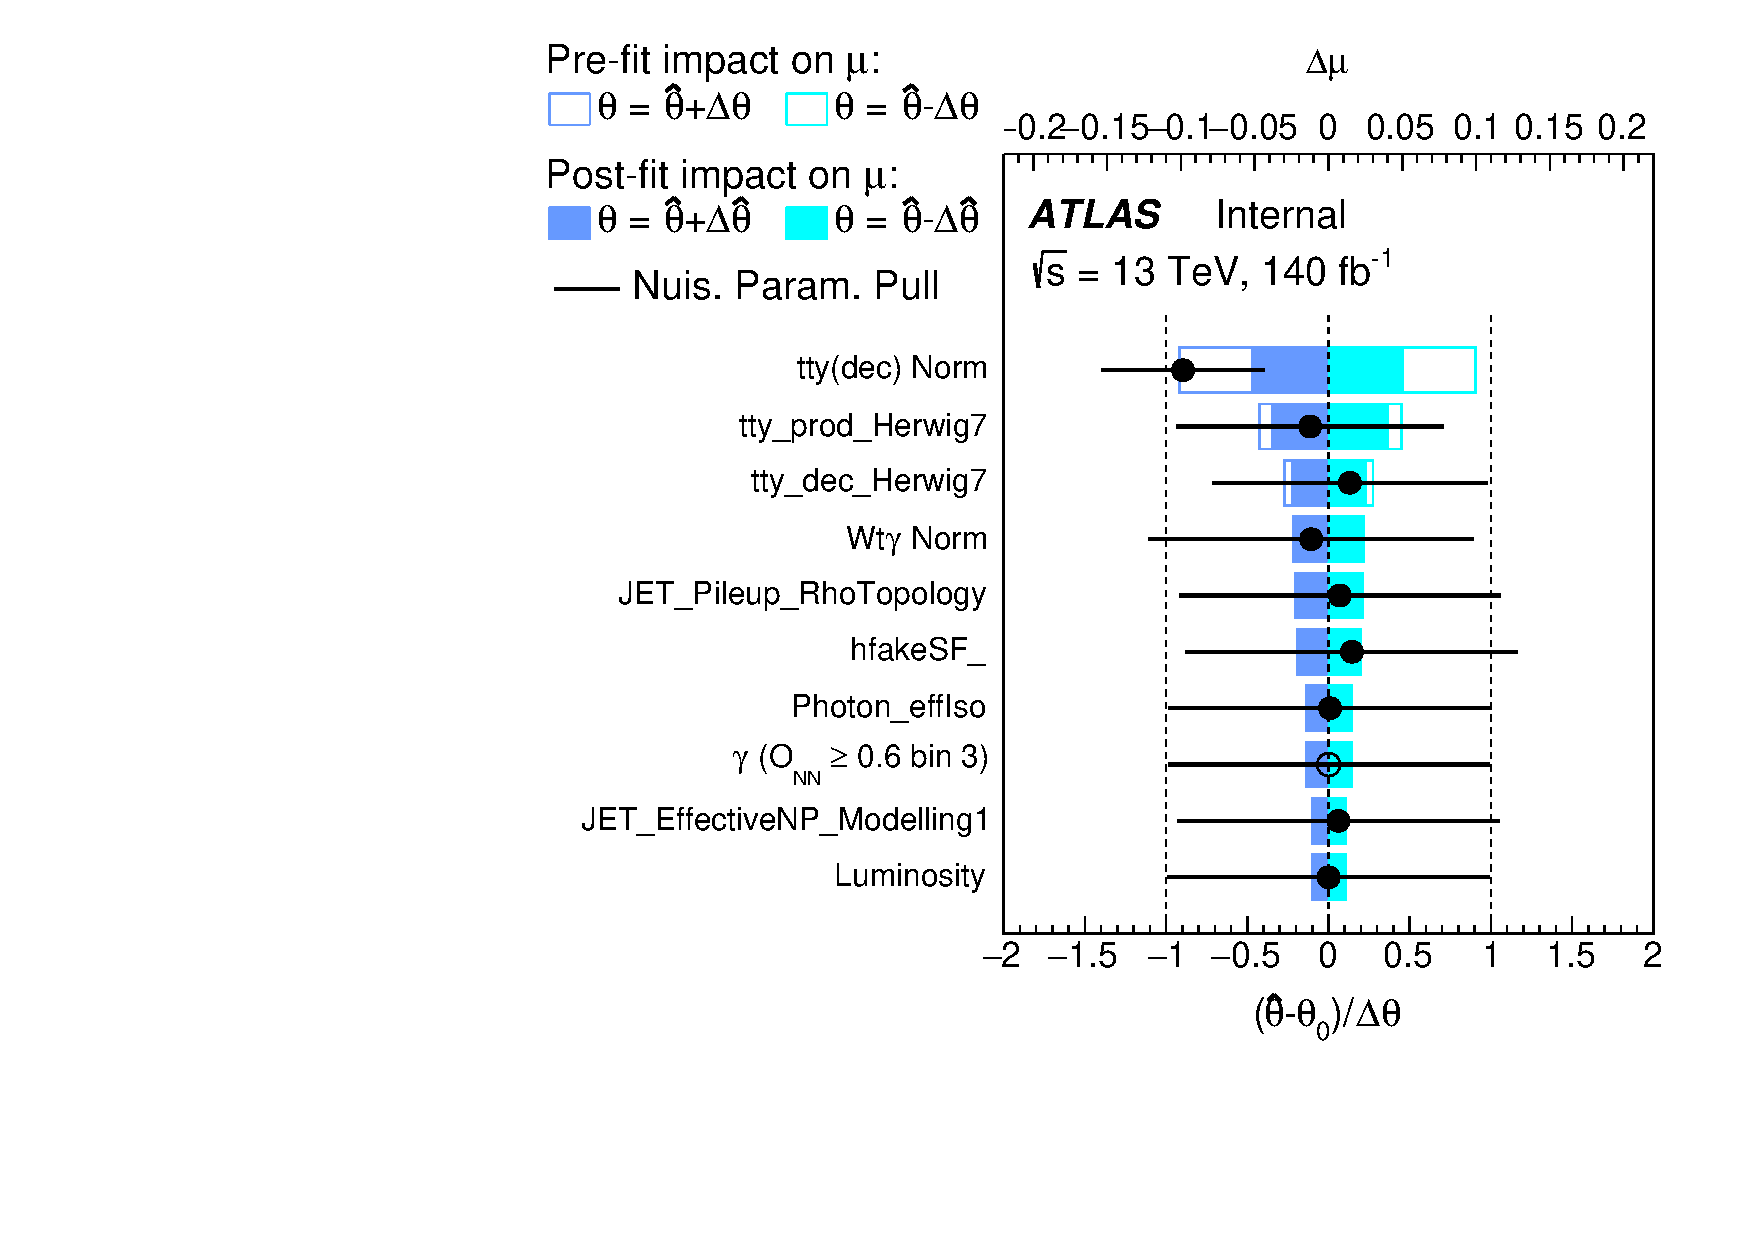
\includegraphics[width=0.2\textwidth]{figures/diff_xsec/dilep_tty_total_mu_blinded/Ranking/tty2l_pt_all_syst/Ranking_tty2l_pt_all_syst_Bin_004_mu.pdf}}
  \quad
  \subfloat[]{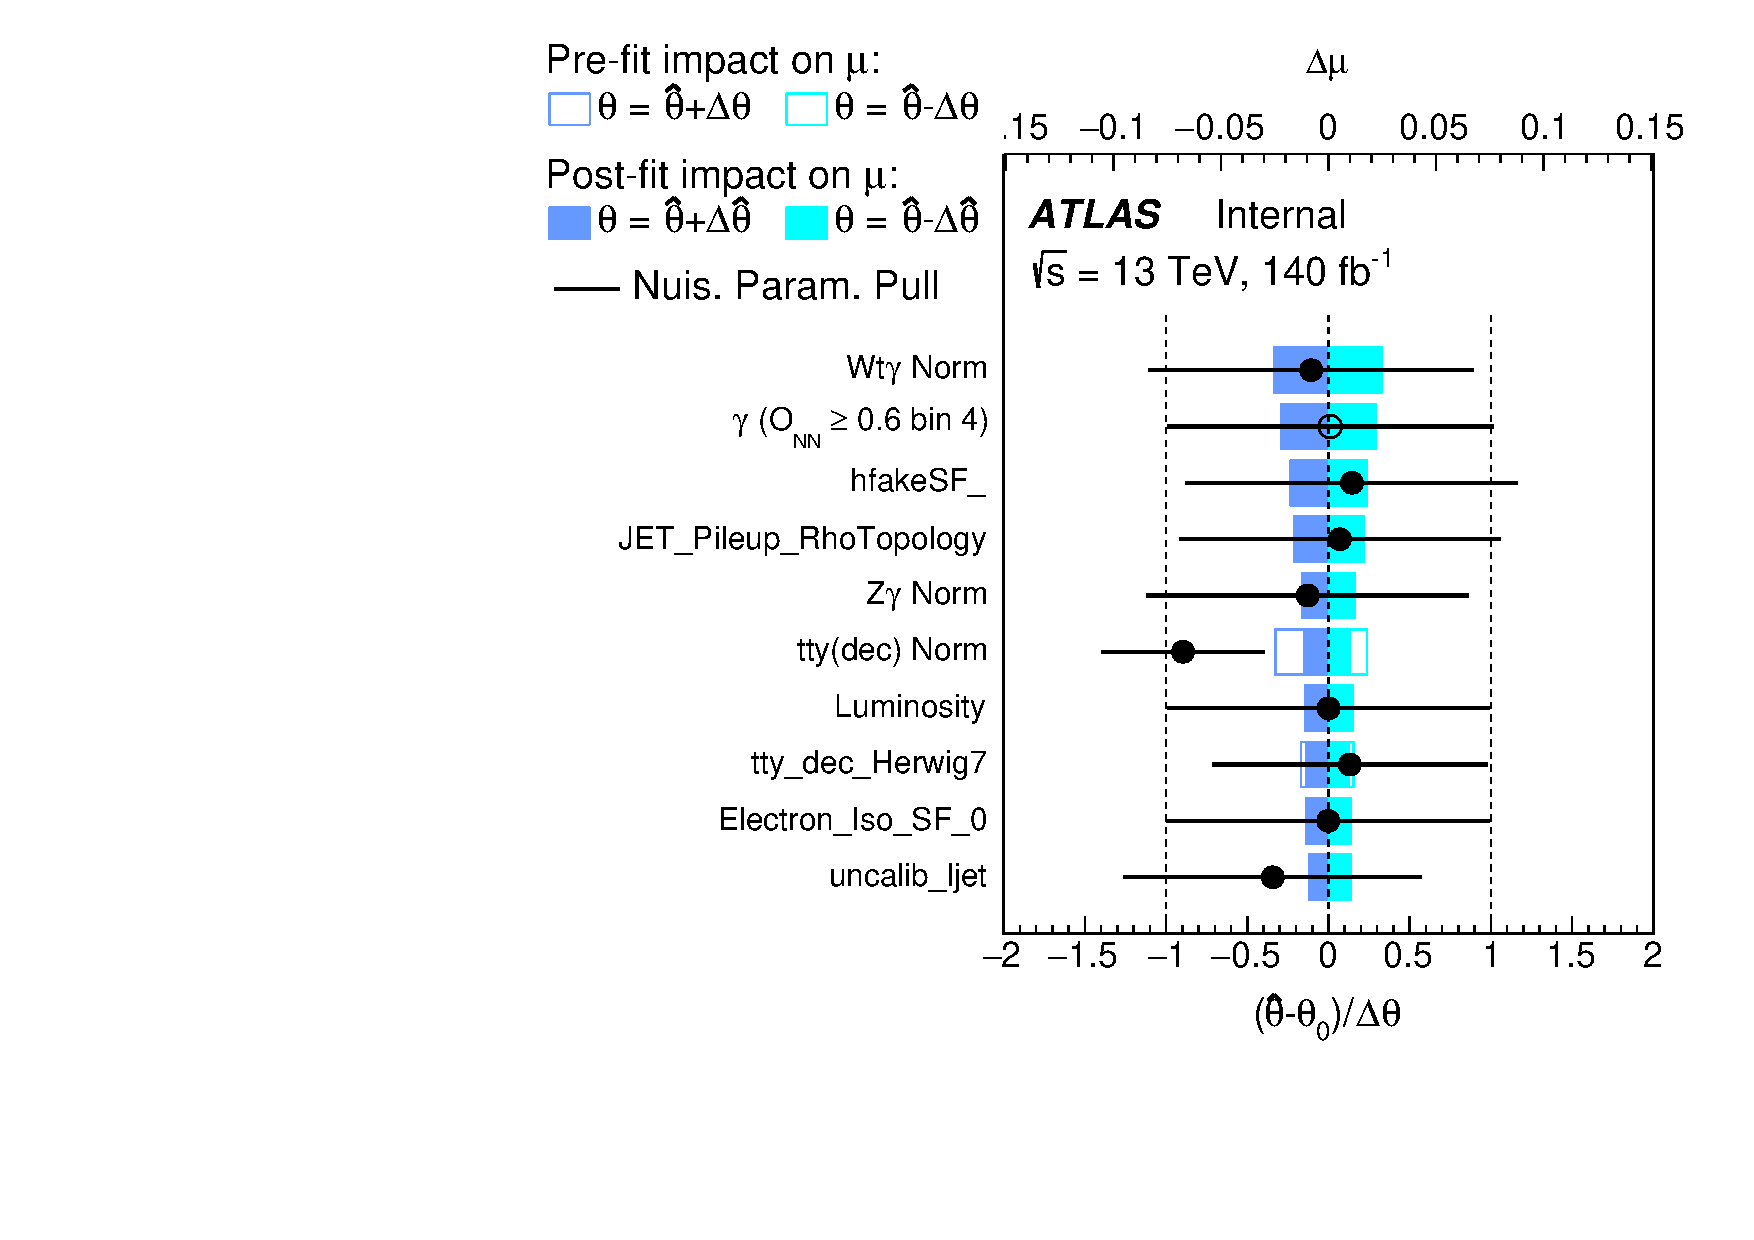
\includegraphics[width=0.2\textwidth]{figures/diff_xsec/dilep_tty_total_mu_blinded/Ranking/tty2l_pt_all_syst/Ranking_tty2l_pt_all_syst_Bin_005_mu.pdf}}
  \quad
  \subfloat[]{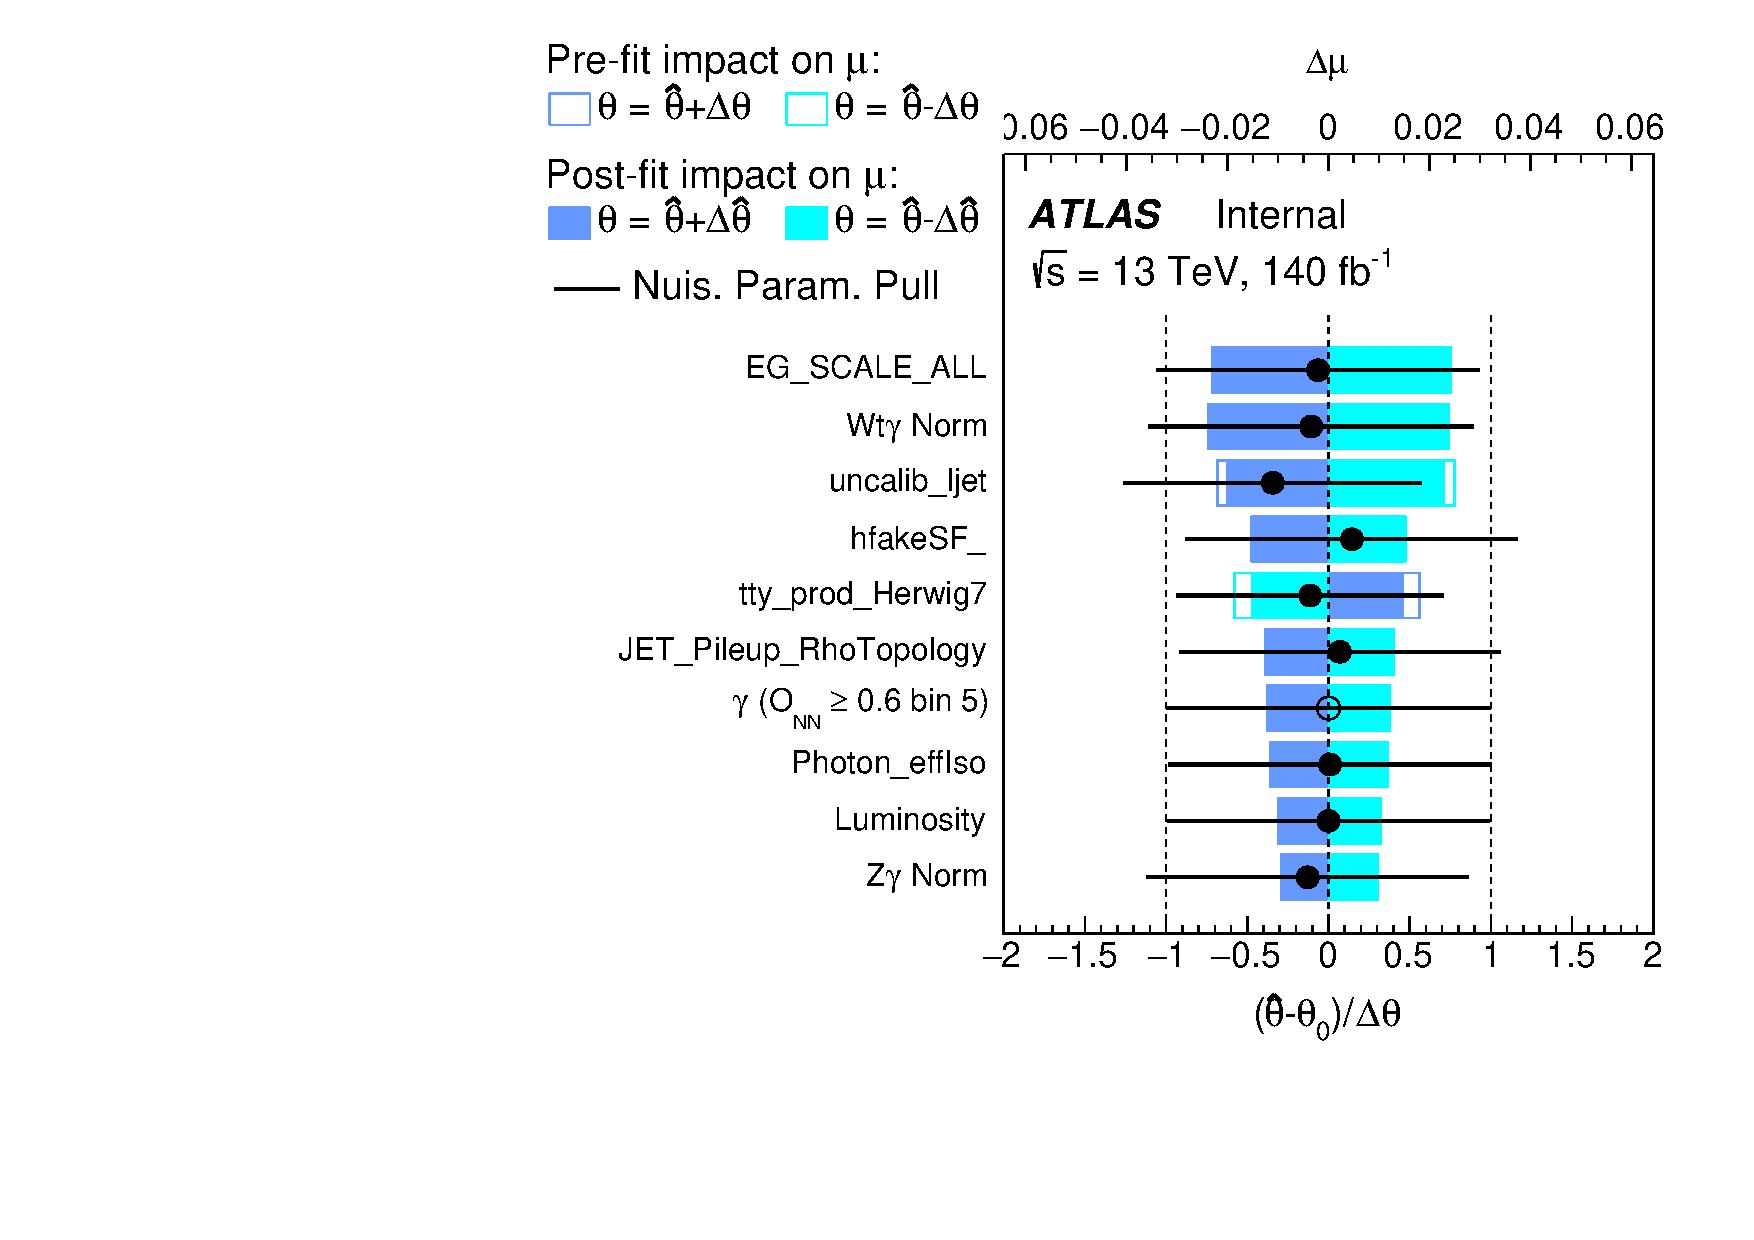
\includegraphics[width=0.2\textwidth]{figures/diff_xsec/dilep_tty_total_mu_blinded/Ranking/tty2l_pt_all_syst/Ranking_tty2l_pt_all_syst_Bin_006_mu.pdf}}
  \caption{Ranking plots of the 10 NPs with the largest impact on the \tty (total) signal strength in each bin of the $p_T(\gamma)$ distribution in the dilepton channel. 
  The fit was performed to the data keeping the POIs blinded. Each subfigure, labeled (a), (b), (c), (d), (e), and (f), corresponds to a specific bin 
  of the $p_T(\gamma)$ distribution, with bin 1 (lowest \pt) represented in subfigure (a), bin 2 represented in 
  subfigure (b), and so on. }
  \label{fig:ranking_dilep_total_mu_blinded}
\end{figure}
\FloatBarrier

%%%%%%%%%%%% UNFOLDED Distributions %%%%%%%%%%%%%%%%%%%%%
\begin{figure}[ht]
  \centering
  \subfloat[]{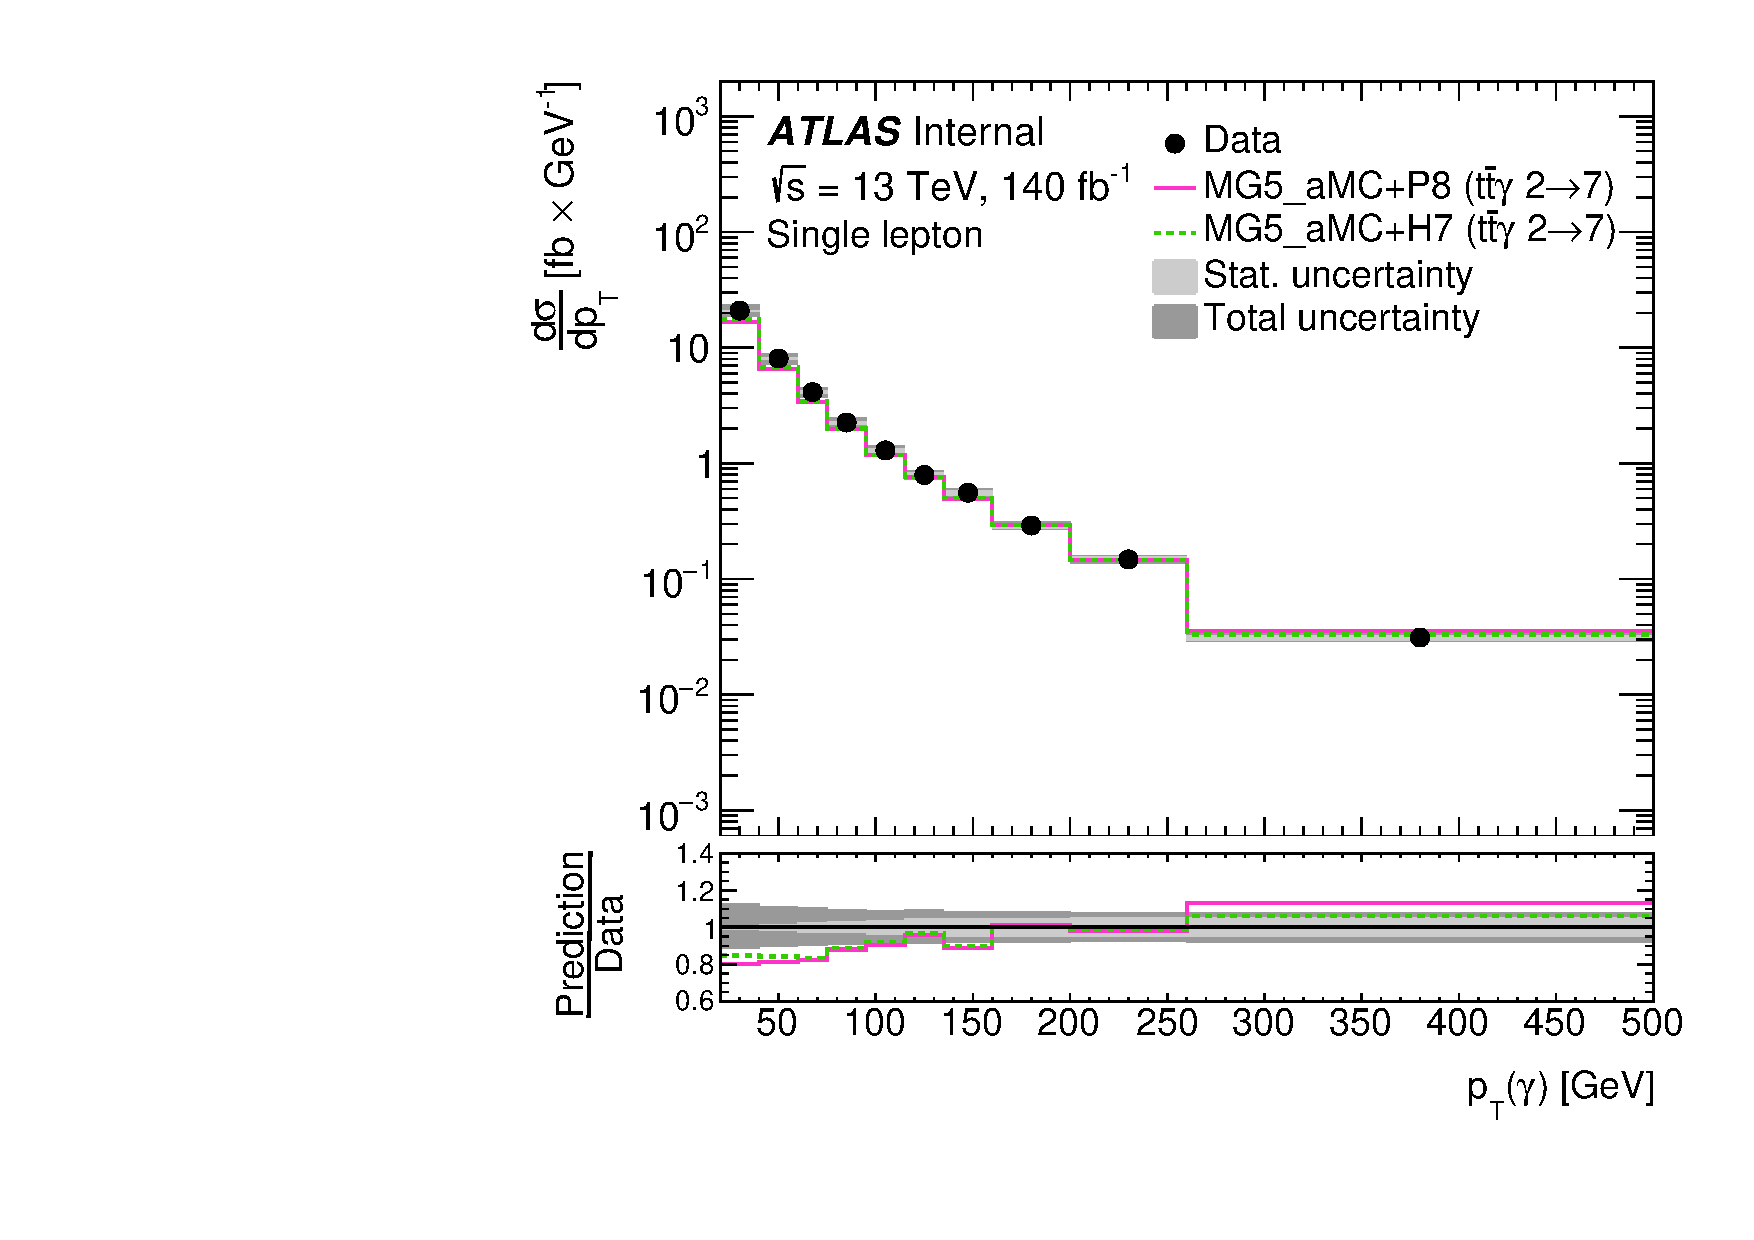
\includegraphics[width=0.4\textwidth]{figures/diff_xsec/absolute-unfolded-distributions/tty_total_ljet/SL_tty_total_pt_unfolded_absolute.pdf}}
  \quad\quad
  \subfloat[]{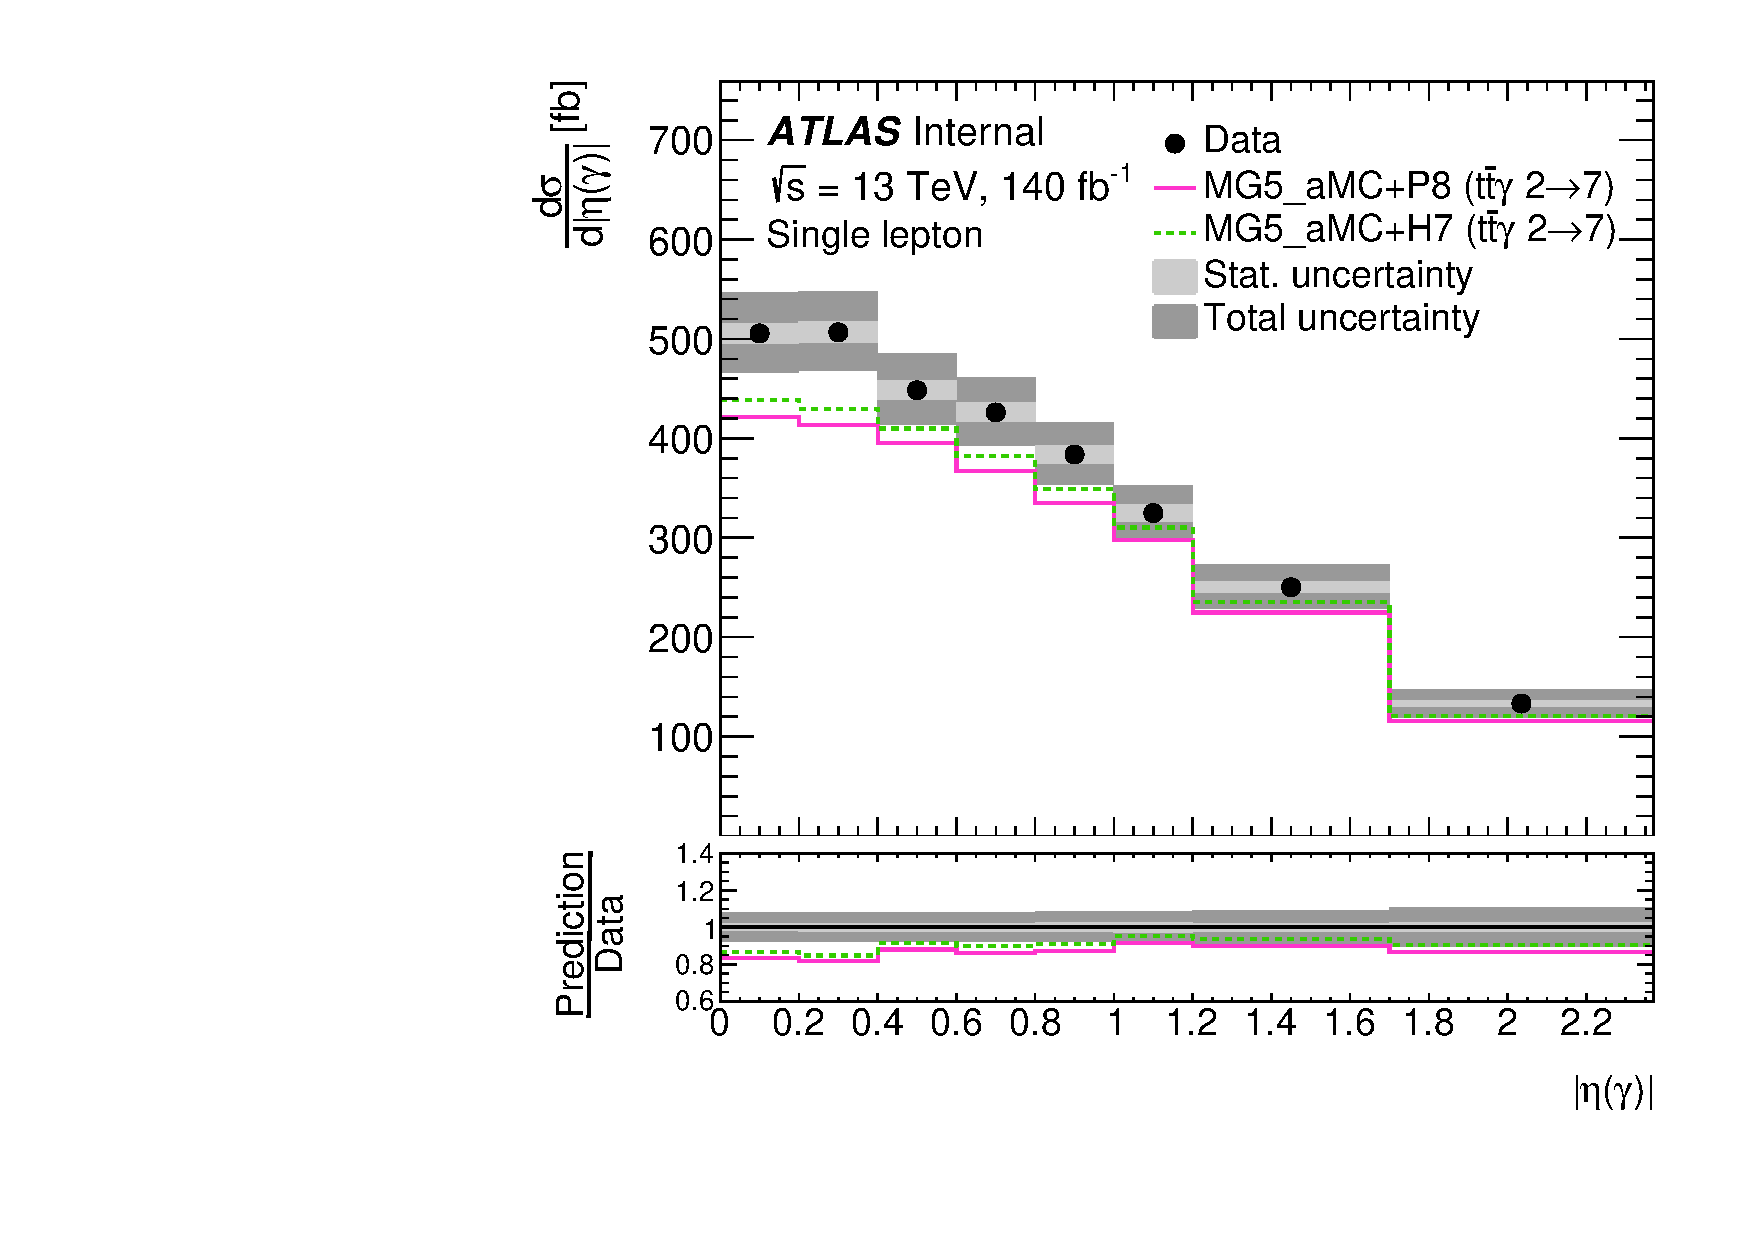
\includegraphics[width=0.4\textwidth]{figures/diff_xsec/absolute-unfolded-distributions/tty_total_ljet/SL_tty_total_eta_unfolded_absolute.pdf}}
  \quad\quad
  \subfloat[]{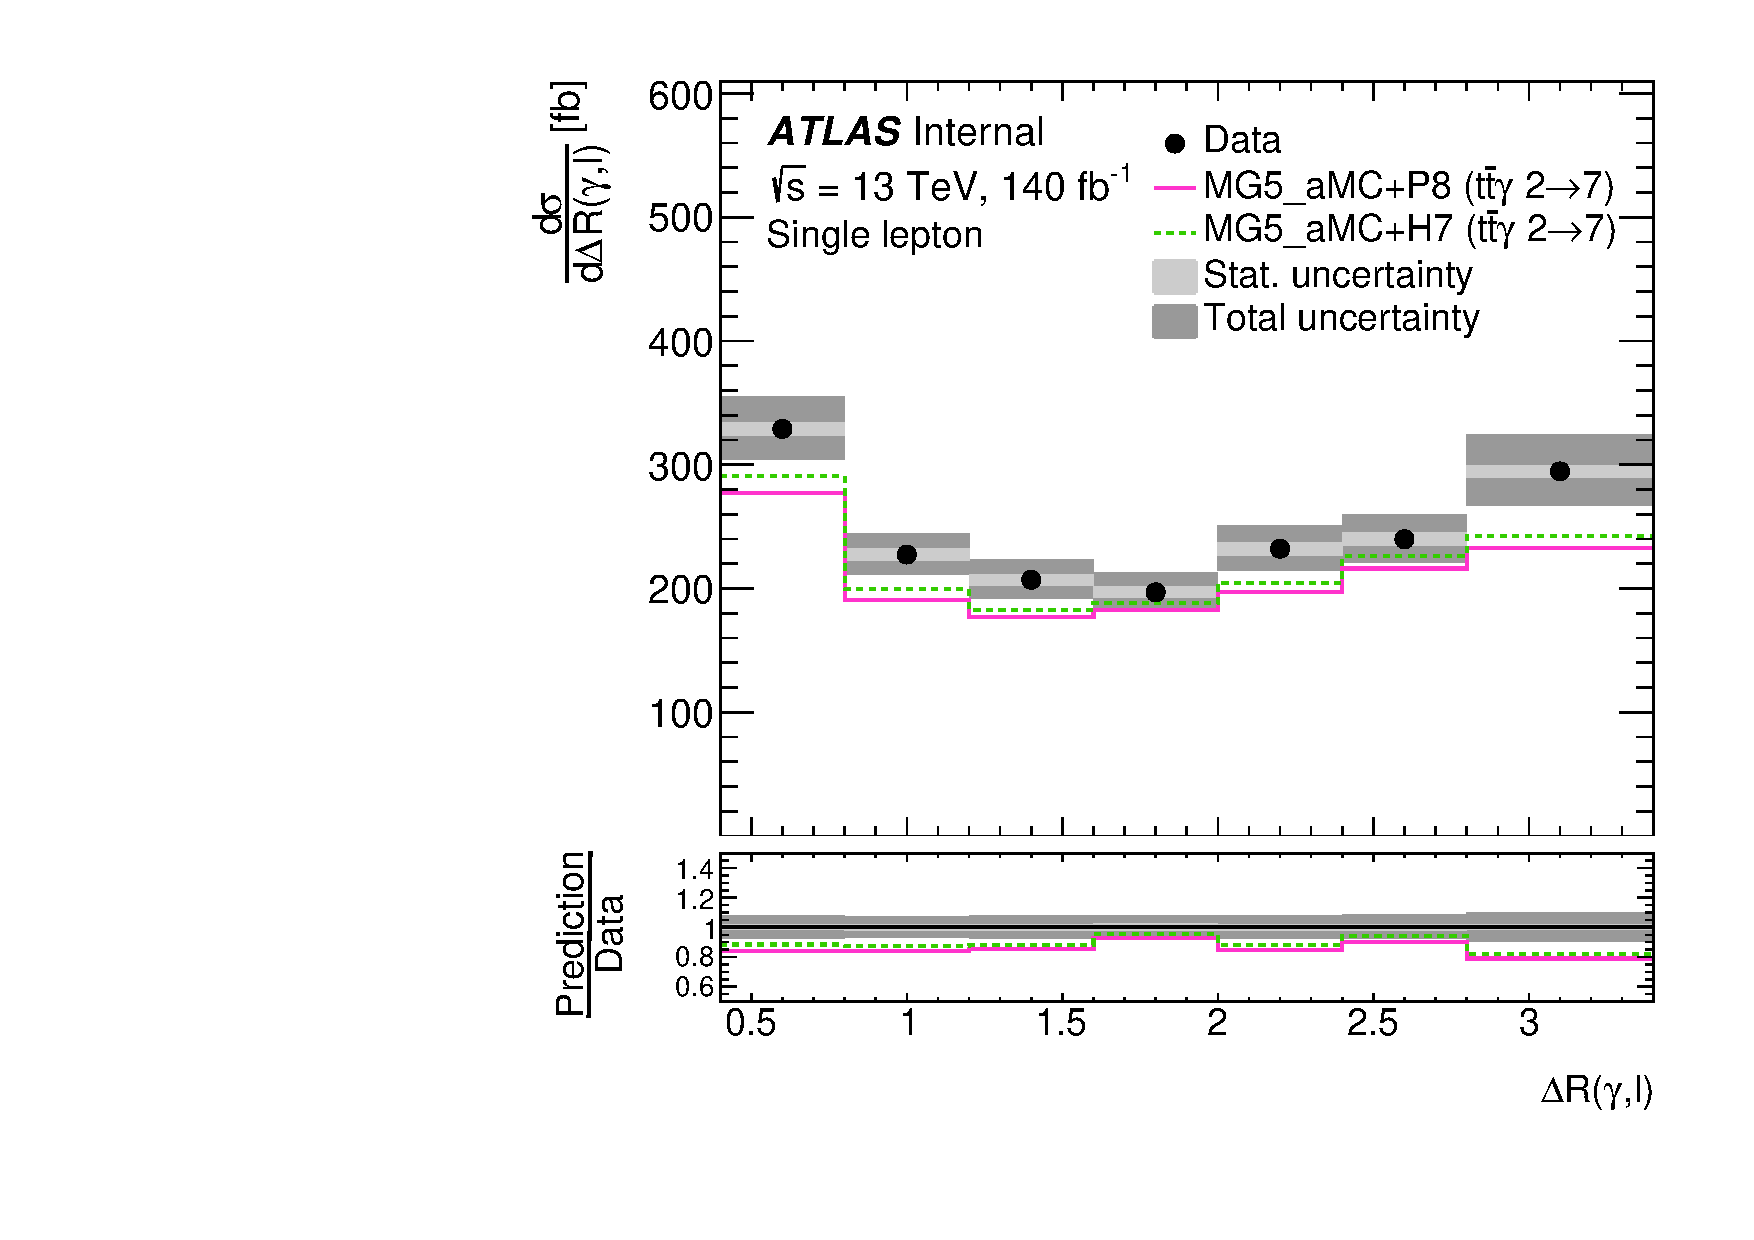
\includegraphics[width=0.4\textwidth]{figures/diff_xsec/absolute-unfolded-distributions/tty_total_ljet/SL_tty_total_drphl_unfolded_absolute.pdf}}
  \quad\quad
  \subfloat[]{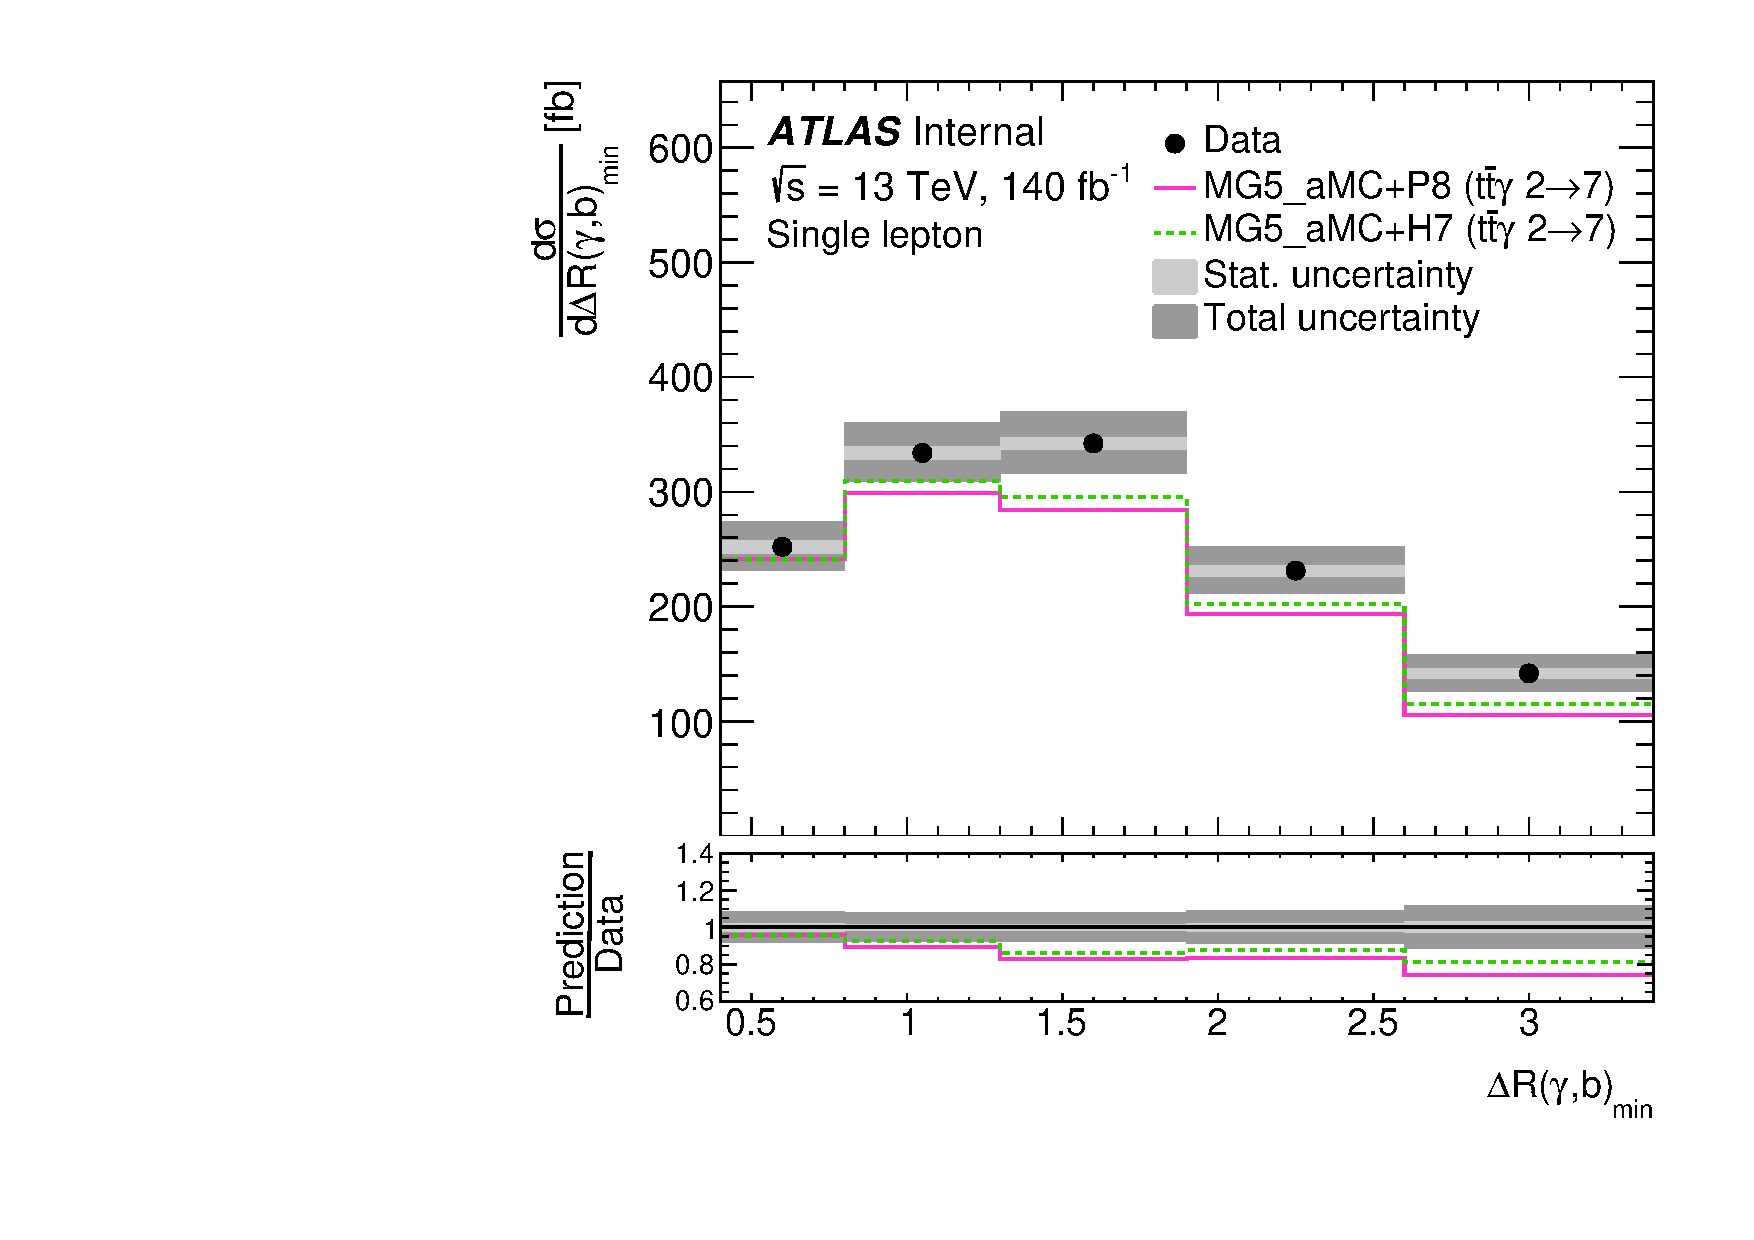
\includegraphics[width=0.4\textwidth]{figures/diff_xsec/absolute-unfolded-distributions/tty_total_ljet/SL_tty_total_drphb_unfolded_absolute.pdf}}
  \quad\quad
  \subfloat[]{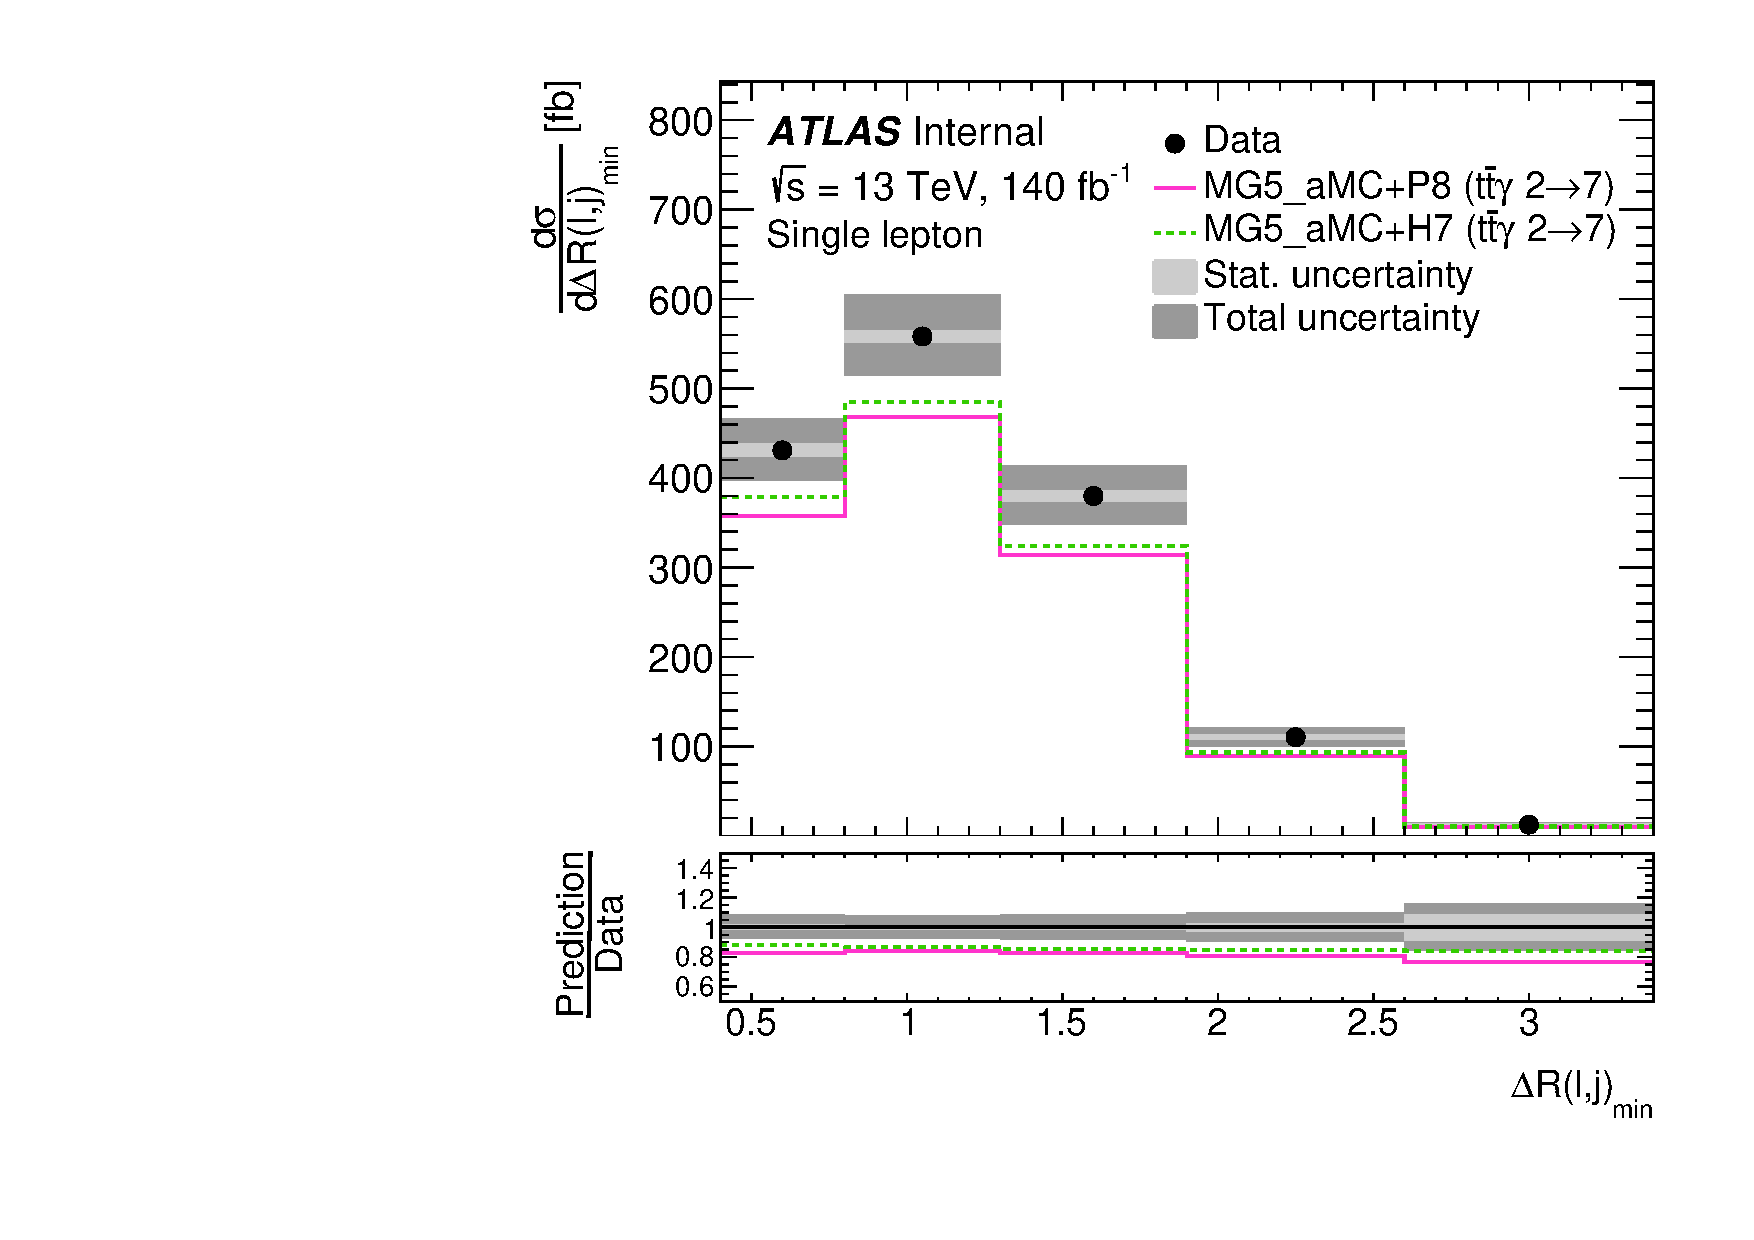
\includegraphics[width=0.4\textwidth]{figures/diff_xsec/absolute-unfolded-distributions/tty_total_ljet/SL_tty_total_drlj_unfolded_absolute.pdf}}
  \quad\quad
  \subfloat[]{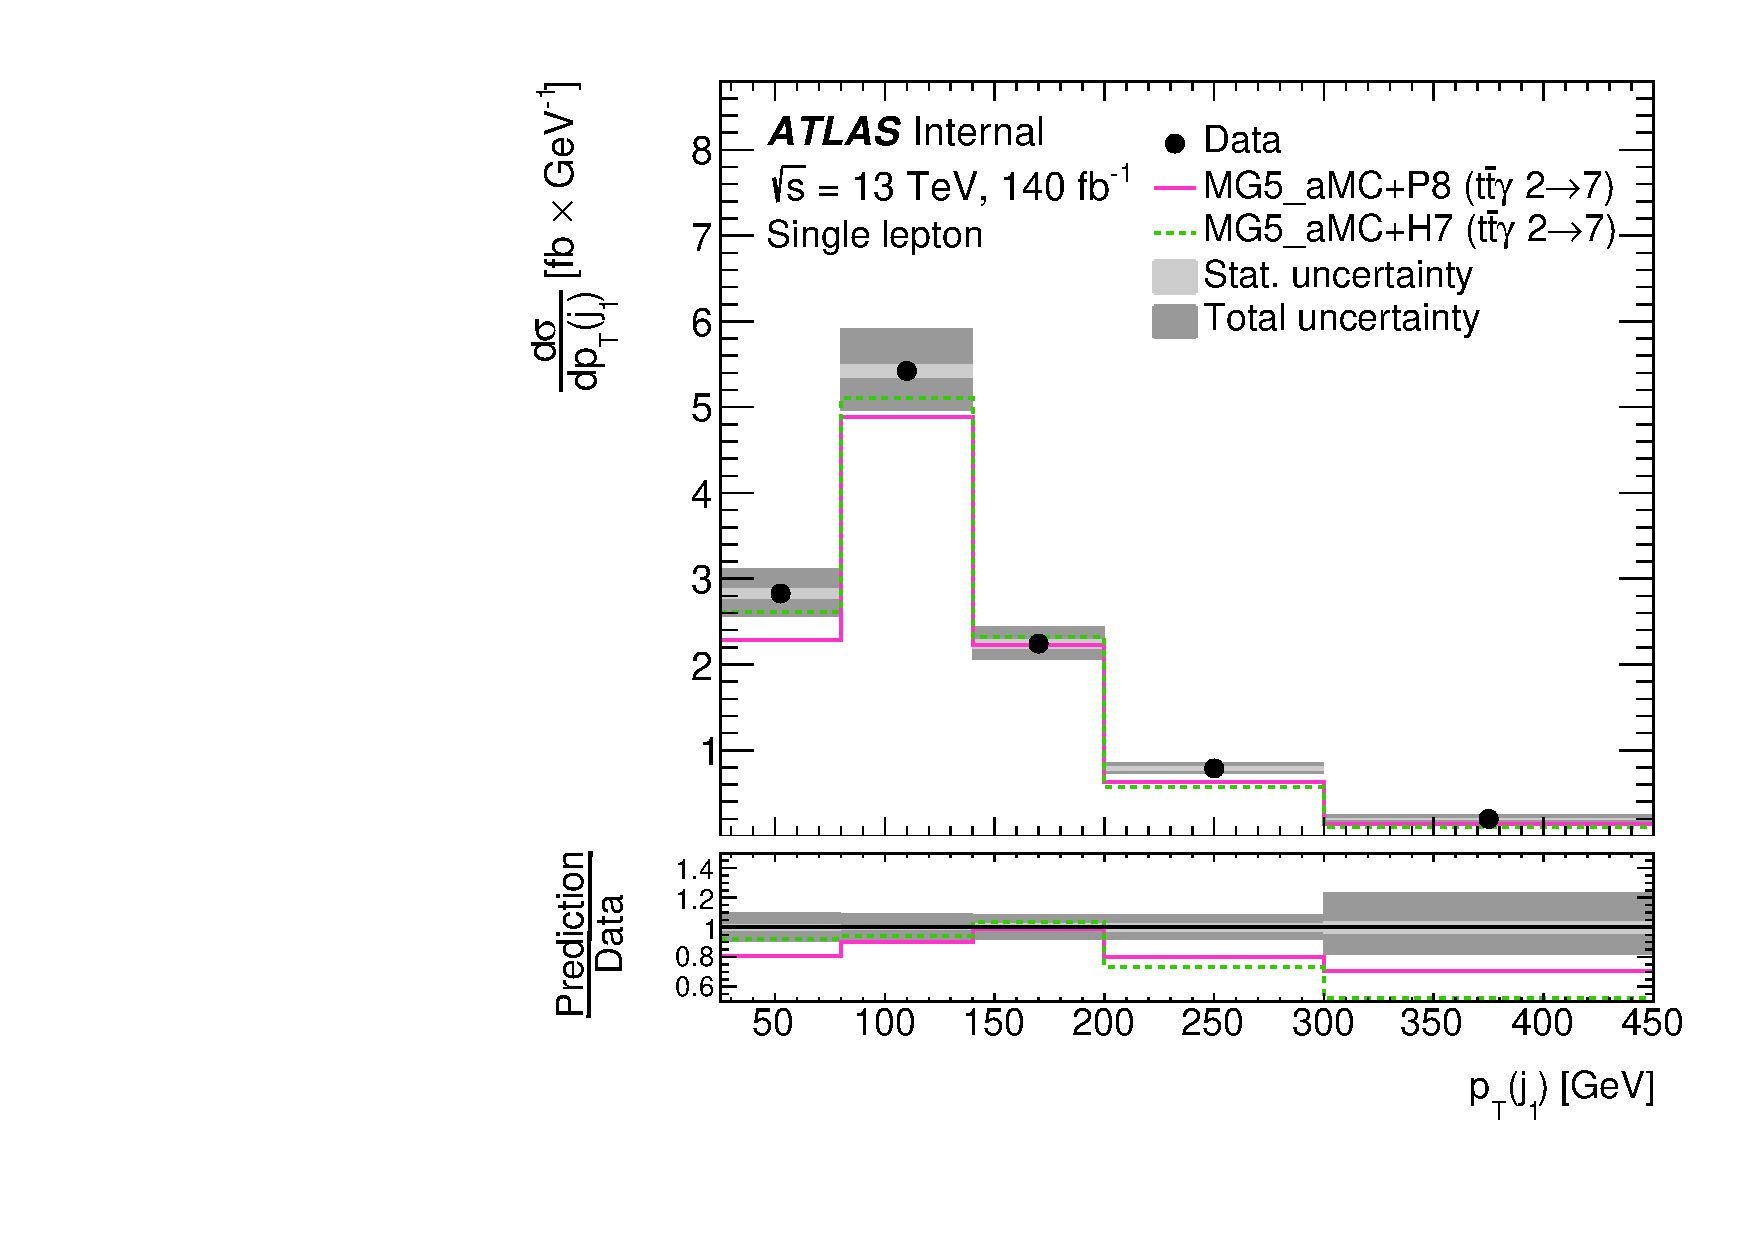
\includegraphics[width=0.4\textwidth]{figures/diff_xsec/absolute-unfolded-distributions/tty_total_ljet/SL_tty_total_ptj1_unfolded_absolute.pdf}}
  \quad\quad
  \caption{For the $t\bar{t}\gamma(\mathrm{total})$ measurement, particle-level unfolded distributions in the single lepton channel after fitting to the real dataset. 
  The error bars represent both statistical and systematic uncertainties. (a) $p_T(\gamma)$, (b) $|\eta(\gamma|)$, 
  (c) $\Delta R_{min}(\gamma, l)$, (d) $\Delta R(\gamma, b)$, (e) $\Delta R_{min}(l, j)$, (f) $p_T(j1)$. Overflow events are included in the last bin of the corresponding distribution.}
  \label{fig:pt_unfolded_ljet_tty_total_realdata}
\end{figure}
\FloatBarrier



\begin{figure}[ht]
  \centering
  \subfloat[]{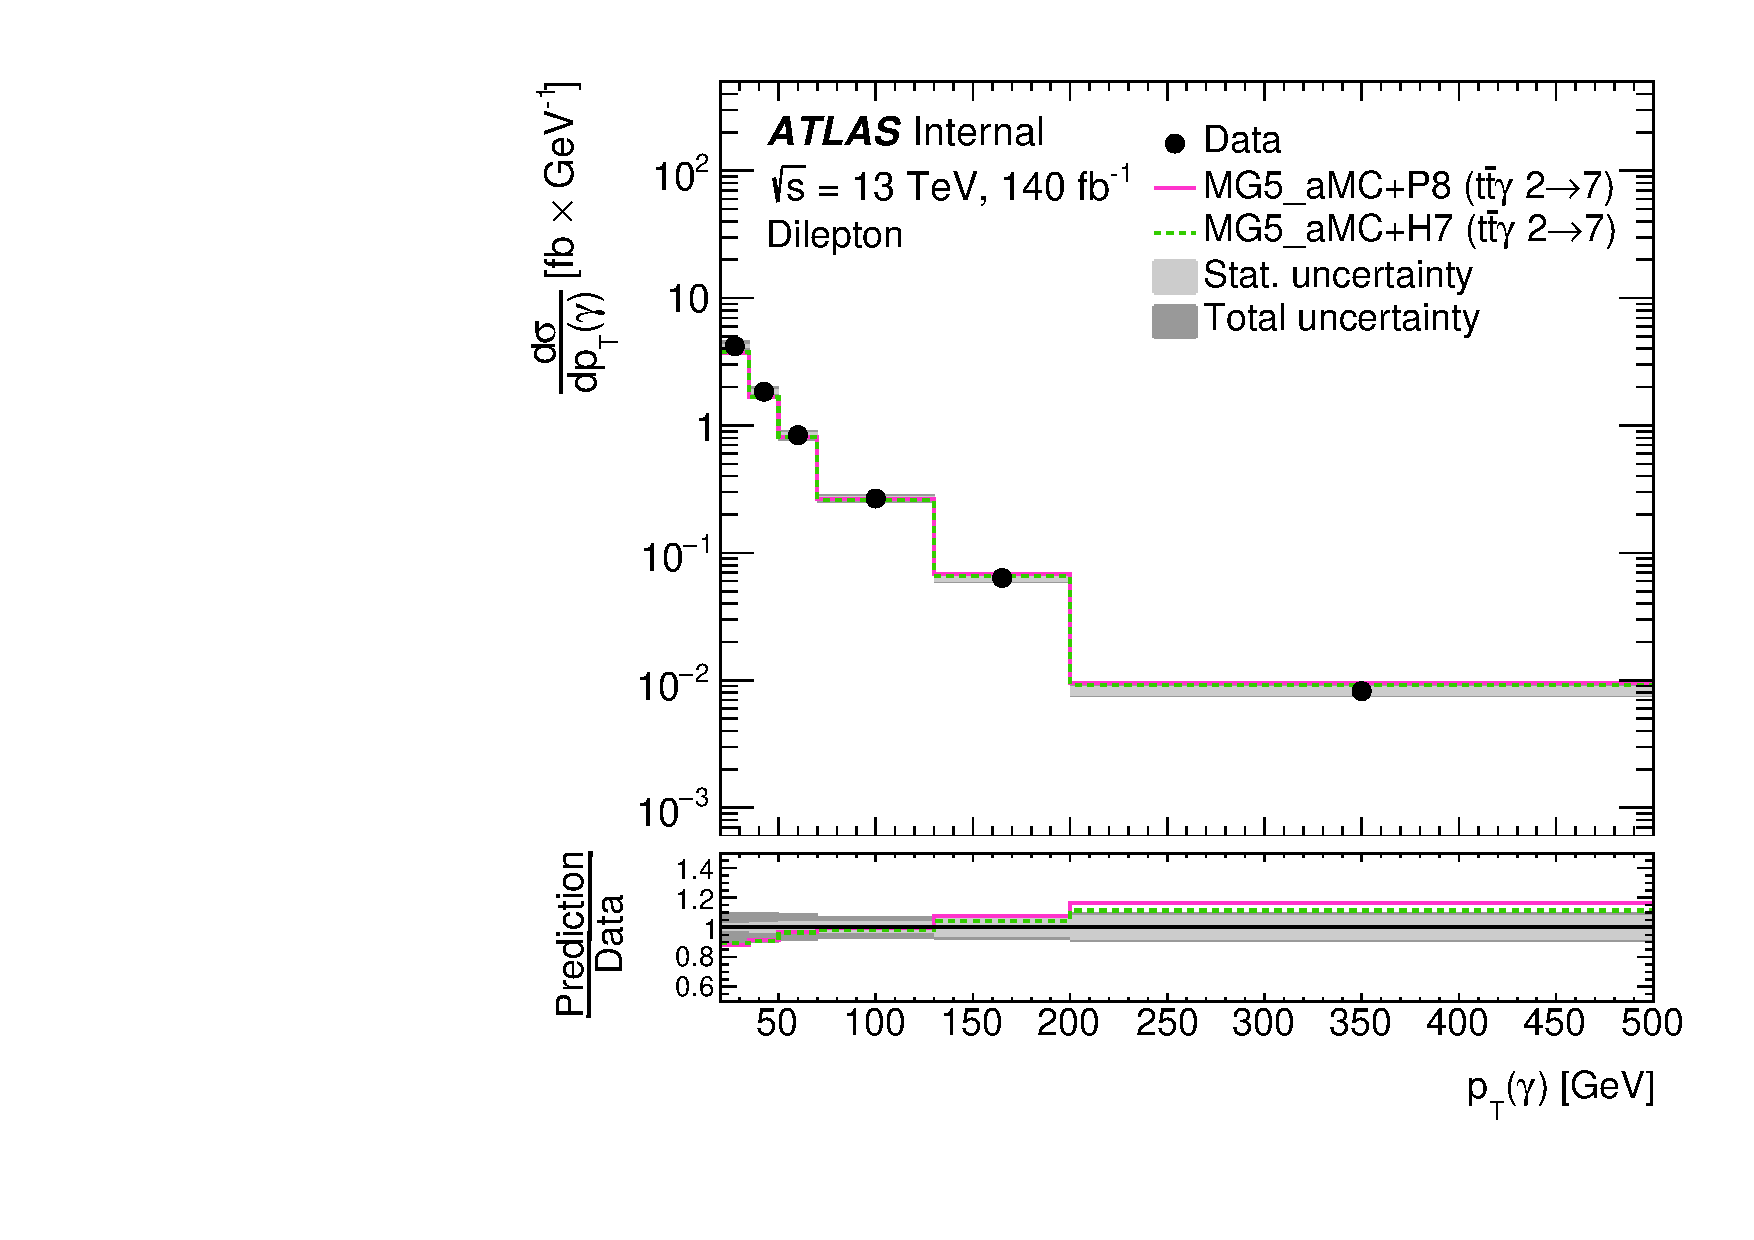
\includegraphics[width=0.4\textwidth]{figures/diff_xsec/absolute-unfolded-distributions/tty_total_dilep/DL_tty_total_pt_unfolded_absolute.pdf}}
  \quad\quad
  \subfloat[]{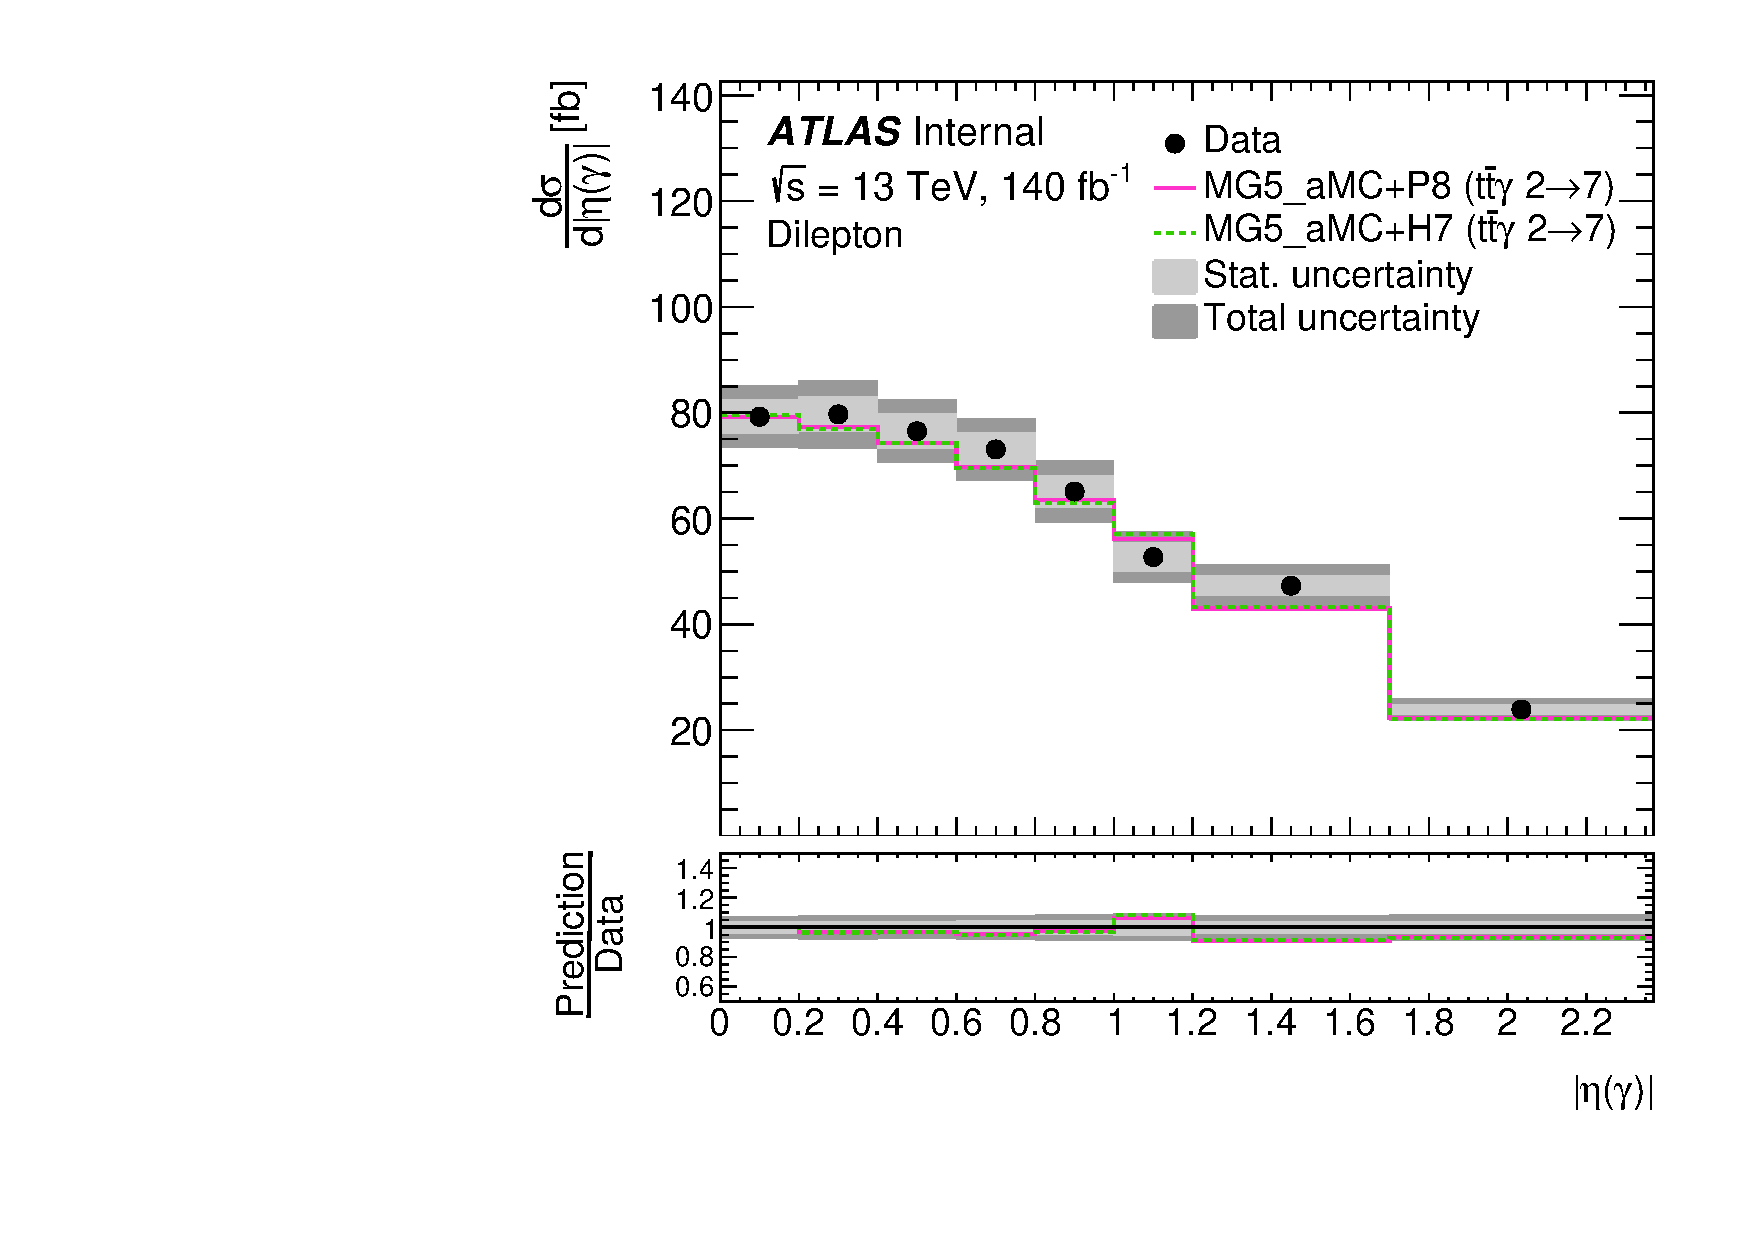
\includegraphics[width=0.4\textwidth]{figures/diff_xsec/absolute-unfolded-distributions/tty_total_dilep/DL_tty_total_eta_unfolded_absolute.pdf}}
  \quad\quad
  \subfloat[]{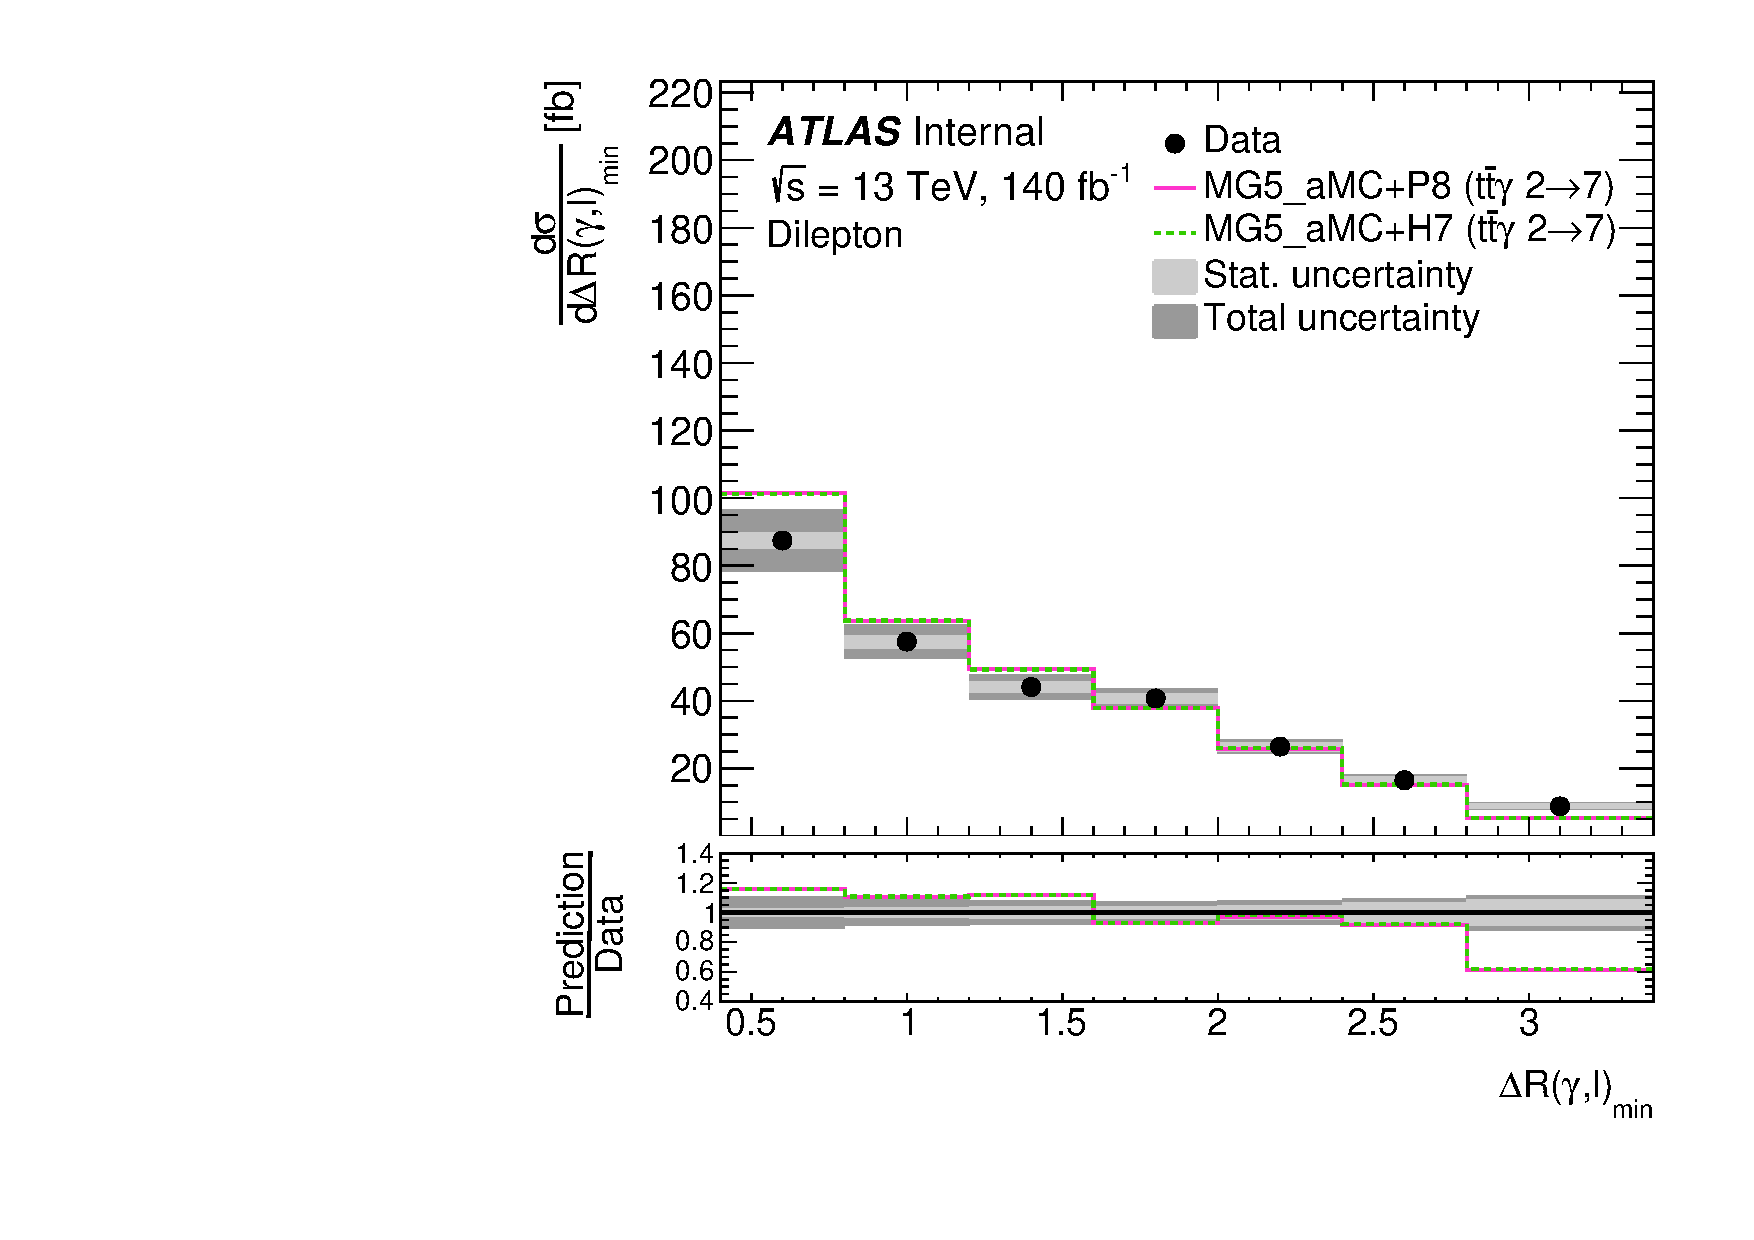
\includegraphics[width=0.4\textwidth]{figures/diff_xsec/absolute-unfolded-distributions/tty_total_dilep/DL_tty_total_drphl_unfolded_absolute.pdf}}
  \quad\quad
  \subfloat[]{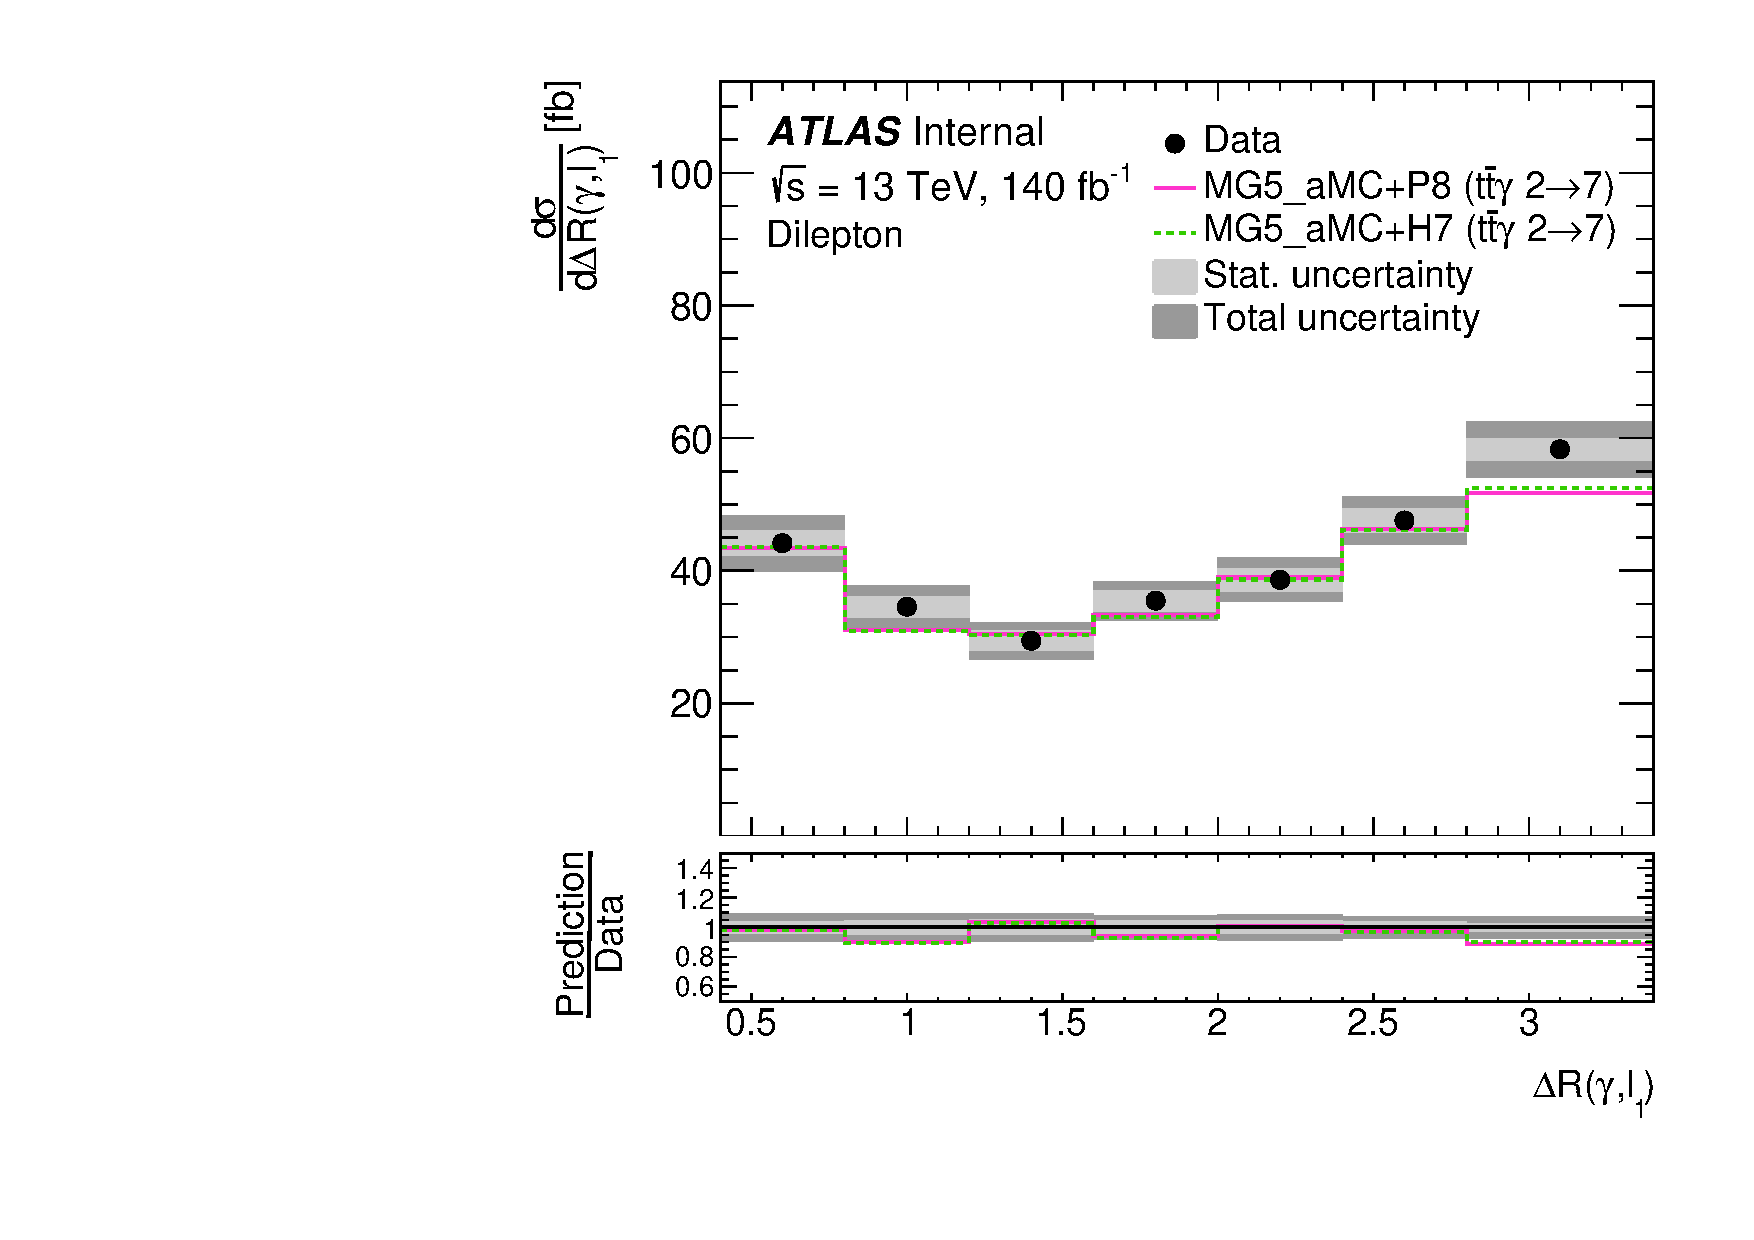
\includegraphics[width=0.4\textwidth]{figures/diff_xsec/absolute-unfolded-distributions/tty_total_dilep/DL_tty_total_drphl1_unfolded_absolute.pdf}}
  \quad\quad
  \subfloat[]{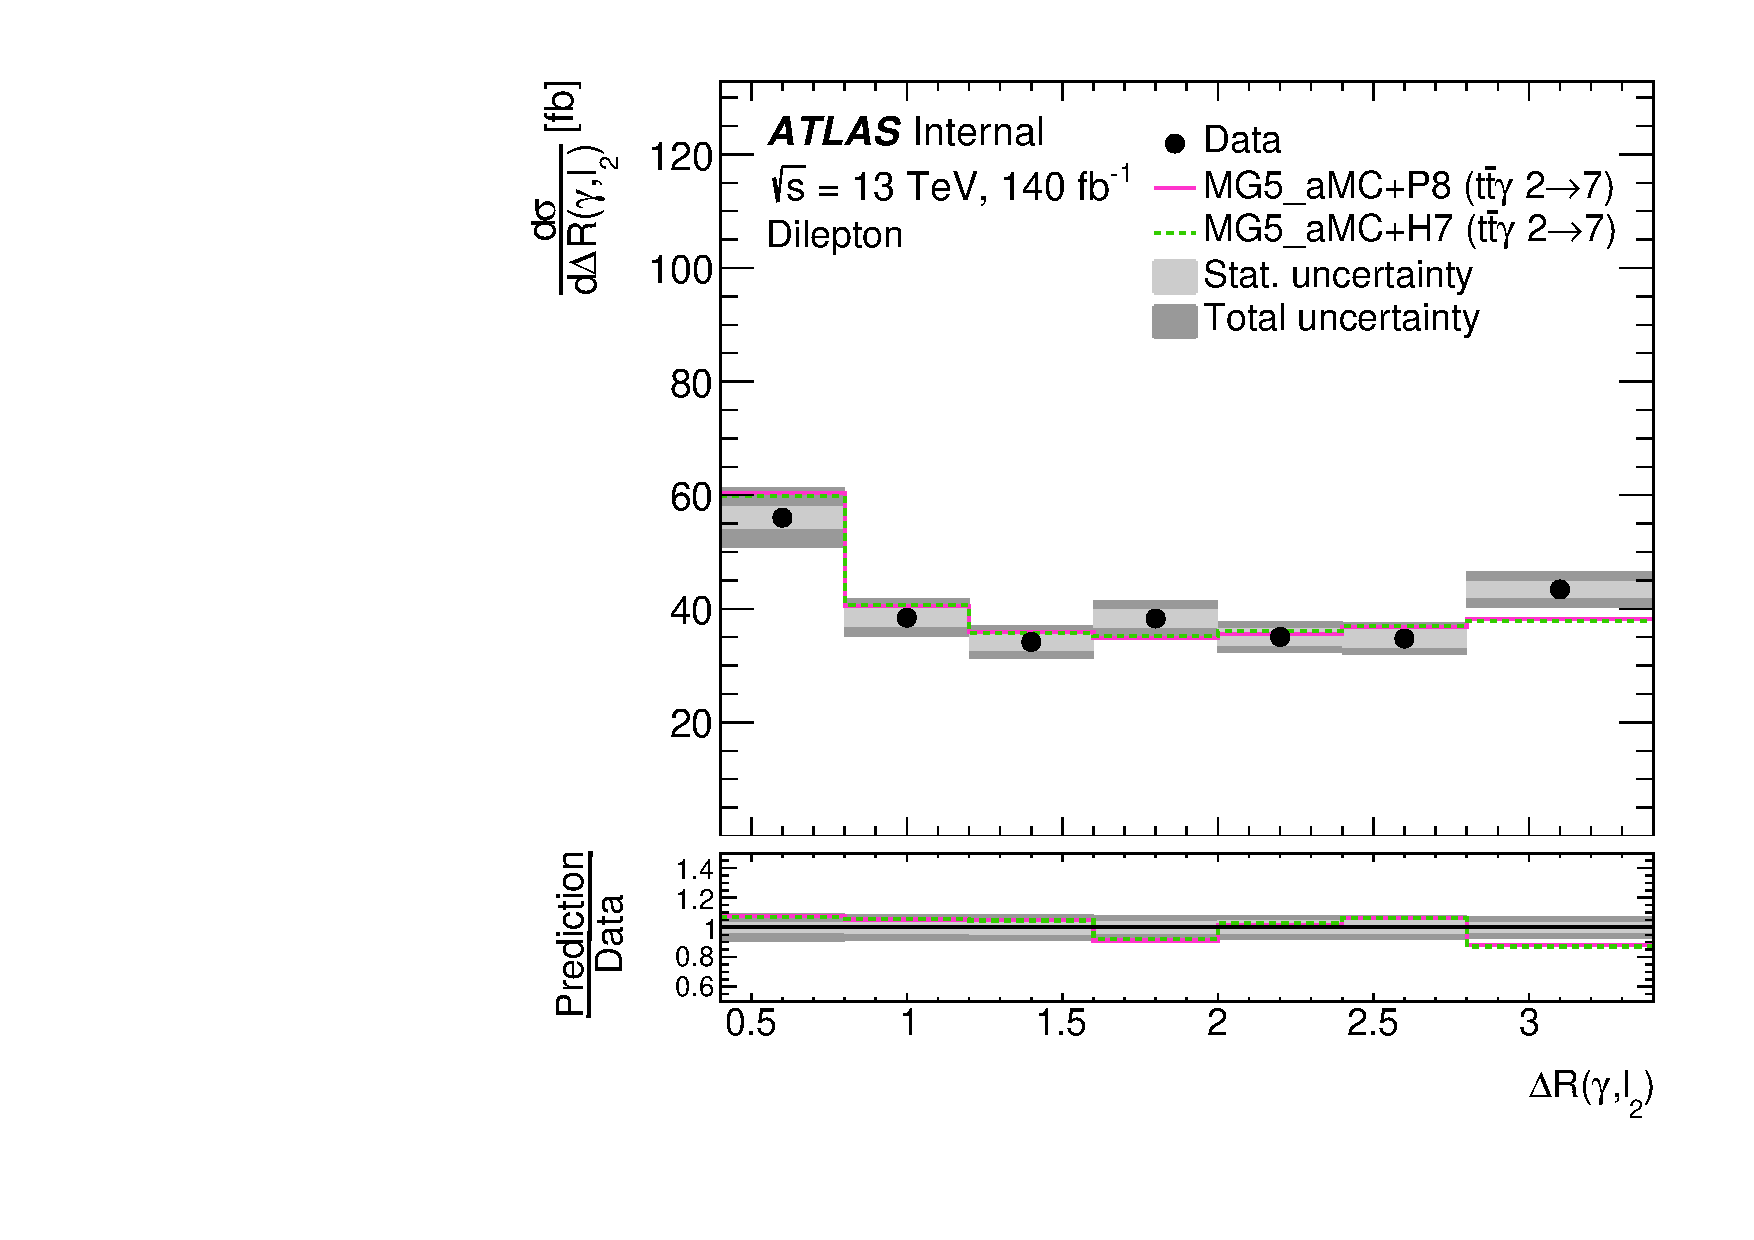
\includegraphics[width=0.4\textwidth]{figures/diff_xsec/absolute-unfolded-distributions/tty_total_dilep/DL_tty_total_drphl2_unfolded_absolute.pdf}}
  \quad\quad
  \subfloat[]{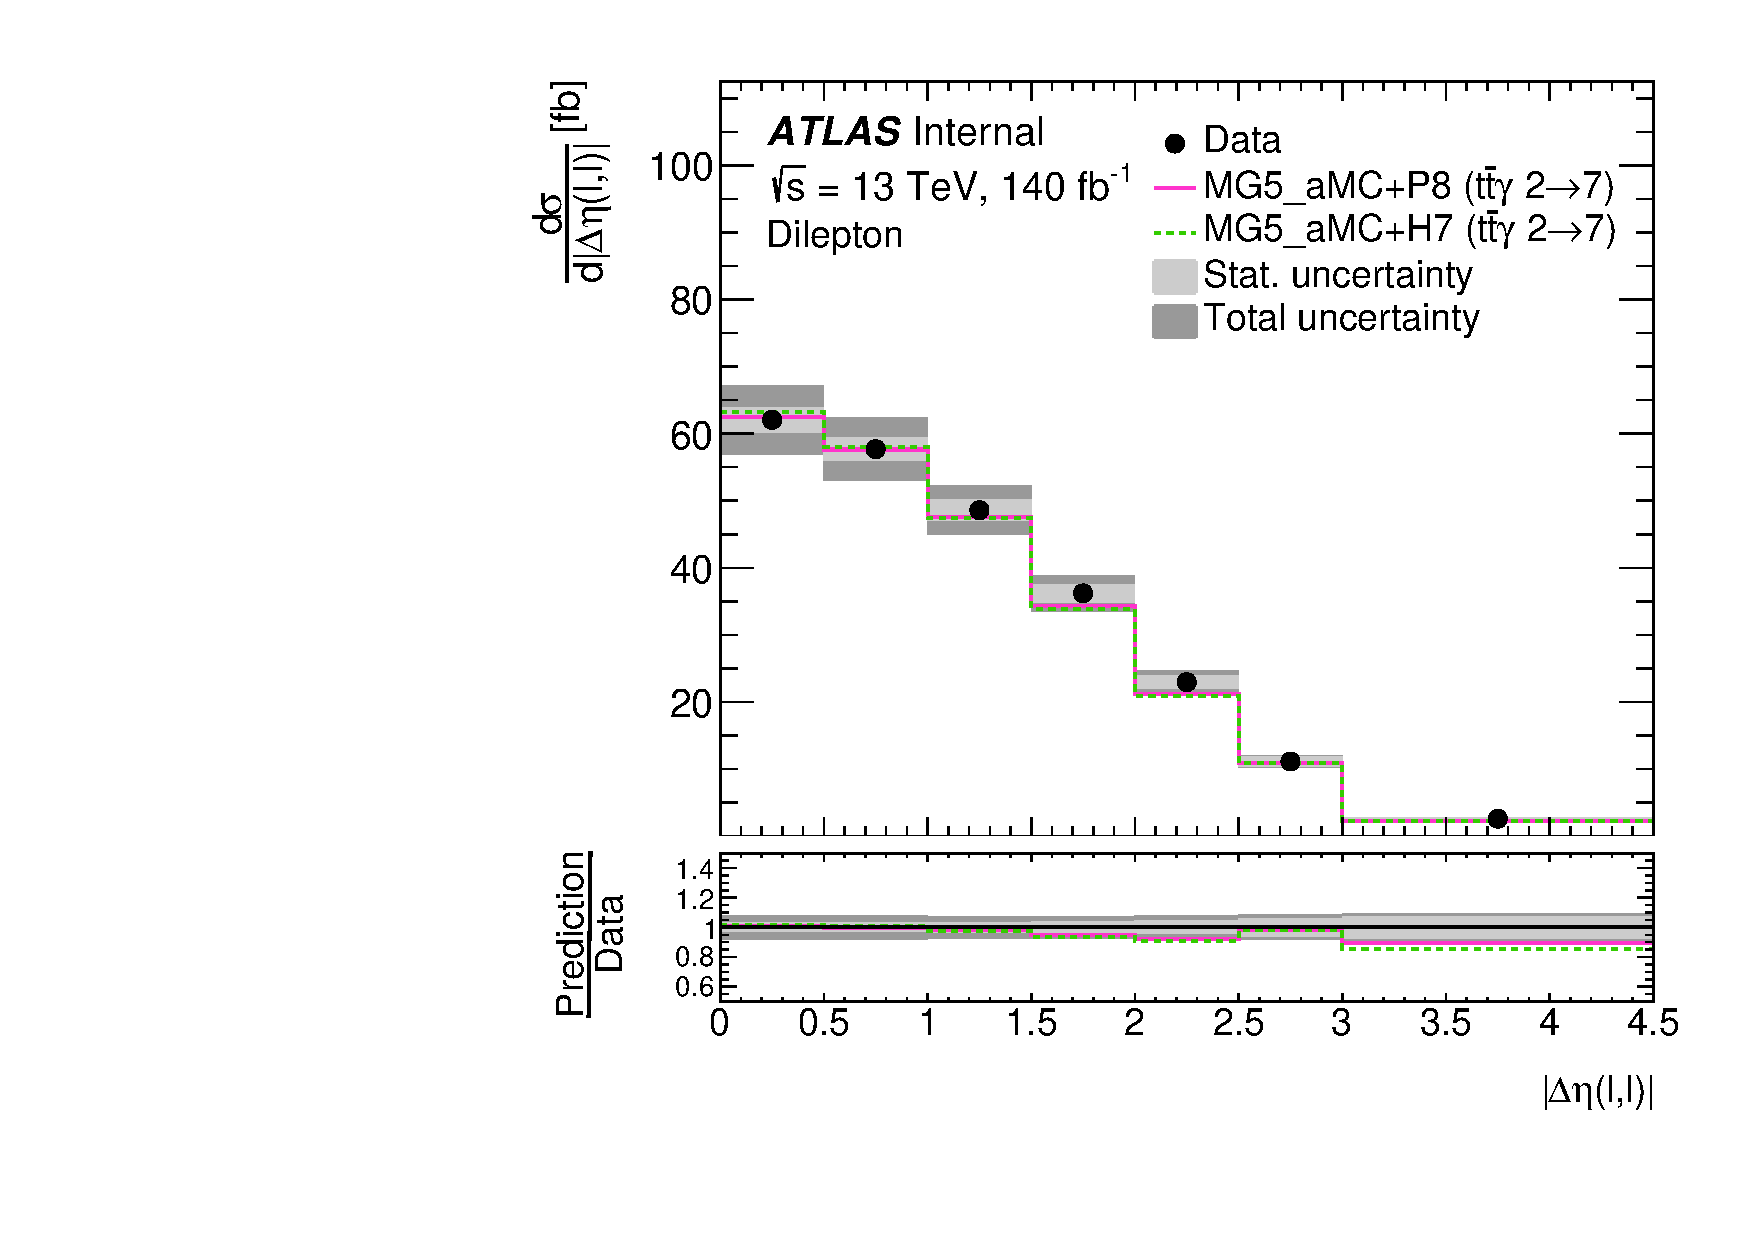
\includegraphics[width=0.4\textwidth]{figures/diff_xsec/absolute-unfolded-distributions/tty_total_dilep/DL_tty_total_dEtall_unfolded_absolute.pdf}}
  \caption{For the $t\bar{t}\gamma(\mathrm{total})$ measurement, particle-level unfolded distributions in the dilepton channel after fitting to the real dataset. 
  The error bars represent both statistical and systematic uncertainties. Overflow events are included in the last bin of the corresponding distribution.}
  \label{fig:pt_unfolded_dilep_tty_total_realdata_1}
\end{figure}

\begin{figure}[ht]
  \centering
  \subfloat[]{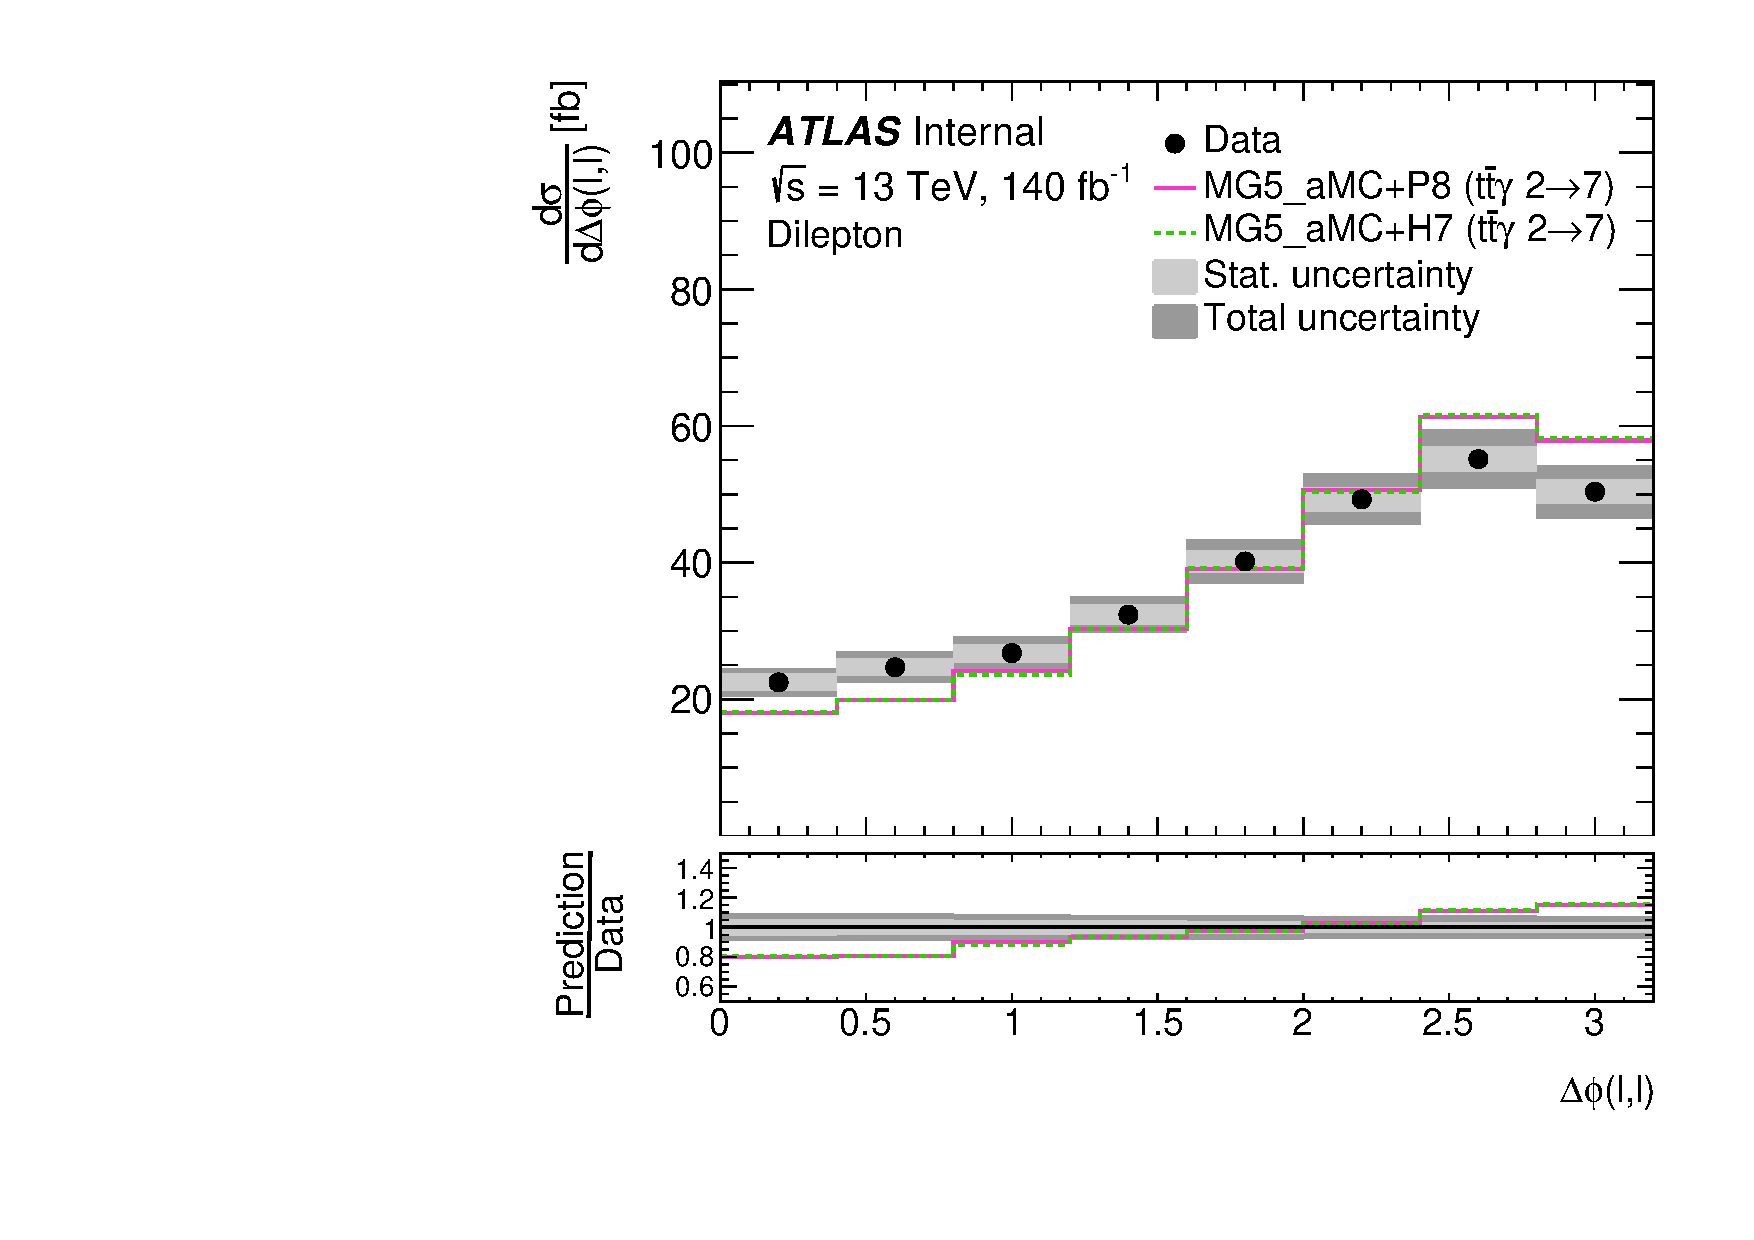
\includegraphics[width=0.4\textwidth]{figures/diff_xsec/absolute-unfolded-distributions/tty_total_dilep/DL_tty_total_dPhill_unfolded_absolute.pdf}}
  \quad\quad
  \subfloat[]{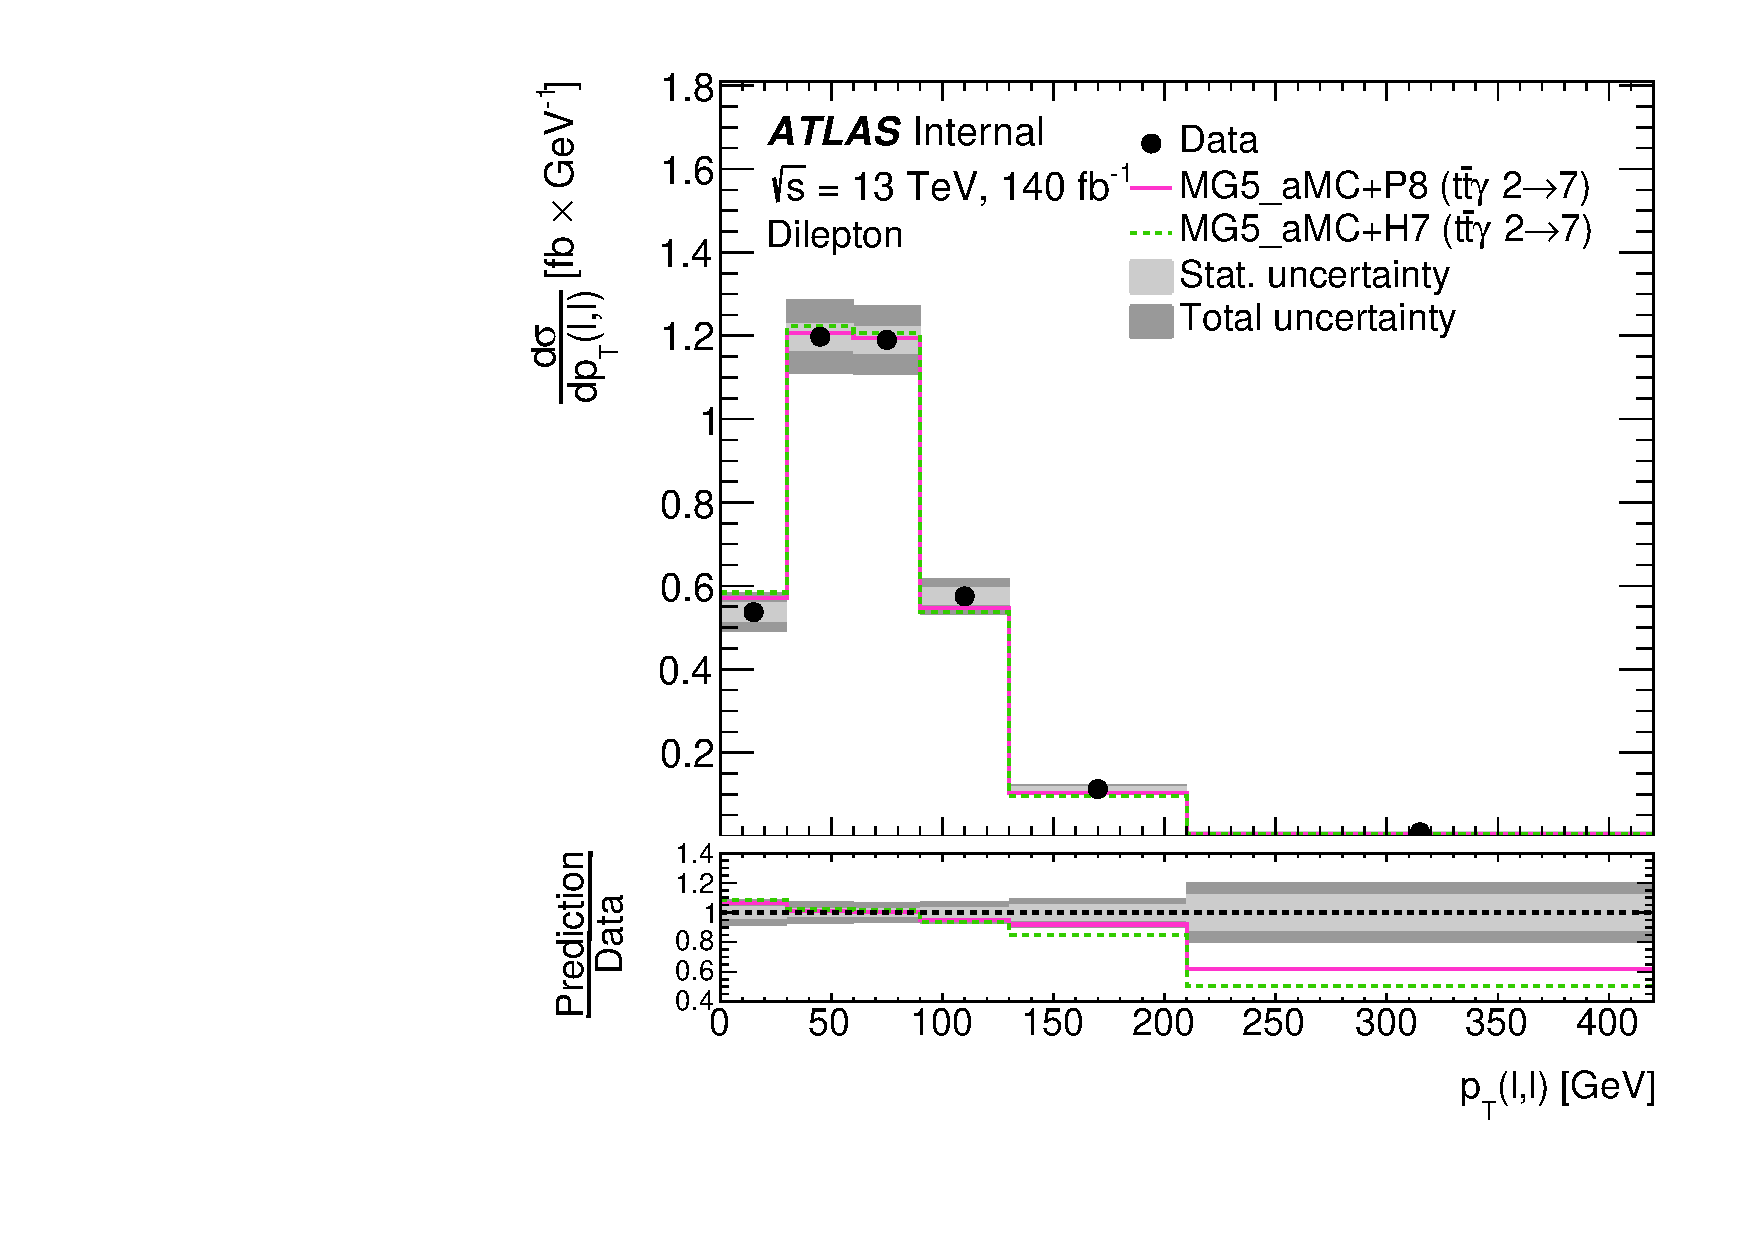
\includegraphics[width=0.4\textwidth]{figures/diff_xsec/absolute-unfolded-distributions/tty_total_dilep/DL_tty_total_ptll_unfolded_absolute.pdf}}
  \quad\quad
  \subfloat[]{\includegraphics[width=0.4\textwidth]{figures/diff_xsec/absolute-unfolded-distributions/tty_total_dilep/DL_tty_total_drphb_unfolded_absolute.pdf}}
  \quad\quad
  \subfloat[]{\includegraphics[width=0.4\textwidth]{figures/diff_xsec/absolute-unfolded-distributions/tty_total_dilep/DL_tty_total_drlj_unfolded_absolute.pdf}}
  \quad\quad
  \subfloat[]{\includegraphics[width=0.4\textwidth]{figures/diff_xsec/absolute-unfolded-distributions/tty_total_dilep/DL_tty_total_ptj1_unfolded_absolute.pdf}}
  \quad\quad
  \caption{For the $t\bar{t}\gamma(\mathrm{total})$ measurement, particle-level unfolded distributions in the dilepton channel after fitting to the real dataset. 
  The error bars represent both statistical and systematic uncertainties. Overflow events are included in the last bin of the corresponding distribution.}
  \label{fig:pt_unfolded_dilep_tty_total_realdata_2}
\end{figure}
\FloatBarrier



%%%%%%%%% NORM FACTORS %%%%%%%%%%%%%%%%

\begin{figure}[ht]
  \centering
  \subfloat[]{\includegraphics[width=0.3\textwidth]{figures/diff_xsec/ljet_tty_total_mu_blinded/Unfolded_data/tty1l_pt_all_syst/NormFactors.pdf}}
  \quad
  \subfloat[]{\includegraphics[width=0.3\textwidth]{figures/diff_xsec/ljet_tty_total_mu_blinded/Unfolded_data/tty1l_eta_all_syst/NormFactors.pdf}}
  \quad
  \subfloat[]{\includegraphics[width=0.3\textwidth]{figures/diff_xsec/ljet_tty_total_mu_blinded/Unfolded_data/tty1l_dr_all_syst/NormFactors.pdf}}
  \quad
  \subfloat[]{\includegraphics[width=0.3\textwidth]{figures/diff_xsec/ljet_tty_total_mu_blinded/Unfolded_data/tty1l_drphb_all_syst/NormFactors.pdf}}
  \quad
  \subfloat[]{\includegraphics[width=0.3\textwidth]{figures/diff_xsec/ljet_tty_total_mu_blinded/Unfolded_data/tty1l_drlj_all_syst/NormFactors.pdf}}
  \quad
  \subfloat[]{\includegraphics[width=0.3\textwidth]{figures/diff_xsec/ljet_tty_total_mu_blinded/Unfolded_data/tty1l_ptj1_all_syst/NormFactors.pdf}}
  \caption{For the $t\bar{t}\gamma(\mathrm{total})$ measurement, the figure displays the normalization factors obtained from the fit to the real dataset for the single 
  lepton channel for the following observables: (a) $p_T(\gamma)$, (b) $|\eta(\gamma|)$, 
  (c) $\Delta R_{min}(\gamma, l)$, (d) $\Delta R(\gamma, b)$, (e) $\Delta R_{min}(l, j)$, (f) $p_T(j1)$.}
  \label{fig:pt_unfolded_ljet_table_tty_total_realdata}
\end{figure}
\FloatBarrier


\begin{figure}[ht]
  \centering
  \subfloat[]{\includegraphics[width=0.3\textwidth]{figures/diff_xsec/dilep_tty_total_mu_blinded/Unfolded_data/tty2l_pt_all_syst/NormFactors.pdf}}
  \quad
  \subfloat[]{\includegraphics[width=0.3\textwidth]{figures/diff_xsec/dilep_tty_total_mu_blinded/Unfolded_data/tty2l_eta_all_syst/NormFactors.pdf}}
  \quad
  \subfloat[]{\includegraphics[width=0.3\textwidth]{figures/diff_xsec/dilep_tty_total_mu_blinded/Unfolded_data/tty2l_dr_all_syst/NormFactors.pdf}}
  \quad
  \subfloat[]{\includegraphics[width=0.3\textwidth]{figures/diff_xsec/dilep_tty_total_mu_blinded/Unfolded_data/tty2l_dr1_all_syst/NormFactors.pdf}}
  \quad
  \subfloat[]{\includegraphics[width=0.3\textwidth]{figures/diff_xsec/dilep_tty_total_mu_blinded/Unfolded_data/tty2l_dr2_all_syst/NormFactors.pdf}}
  \quad
  \subfloat[]{\includegraphics[width=0.3\textwidth]{figures/diff_xsec/dilep_tty_total_mu_blinded/Unfolded_data/tty2l_dEtall_all_syst/NormFactors.pdf}}
  \quad
  \subfloat[]{\includegraphics[width=0.3\textwidth]{figures/diff_xsec/dilep_tty_total_mu_blinded/Unfolded_data/tty2l_dPhill_all_syst/NormFactors.pdf}}
  \quad
  \subfloat[]{\includegraphics[width=0.3\textwidth]{figures/diff_xsec/dilep_tty_total_mu_blinded/Unfolded_data/tty2l_ptll_all_syst/NormFactors.pdf}}
  \quad
  \subfloat[]{\includegraphics[width=0.3\textwidth]{figures/diff_xsec/dilep_tty_total_mu_blinded/Unfolded_data/tty2l_drphb_all_syst/NormFactors.pdf}}
  \quad
  \subfloat[]{\includegraphics[width=0.3\textwidth]{figures/diff_xsec/dilep_tty_total_mu_blinded/Unfolded_data/tty2l_drlj_all_syst/NormFactors.pdf}}
  \subfloat[]{\includegraphics[width=0.3\textwidth]{figures/diff_xsec/dilep_tty_total_mu_blinded/Unfolded_data/tty2l_ptj1_all_syst/NormFactors.pdf}}
  \caption{For the $t\bar{t}\gamma(\mathrm{total})$ measurement, the figure displays the normalisation factors obtained from the fit to the reald dataset for the dilepton channel
  for the following observables: (a) $p_T(\gamma)$, (b) $|\eta(\gamma|)$, (c) $\Delta R_{min}(\gamma, l)$
  (d) $\Delta R(\gamma, l1)$, (e) $\Delta R(\gamma, l2)$, (f) $|\Delta \eta(l, l)|$, (g) $|\Delta \phi(l, l)|$,
  (h) $p_T(ll)$, (i) $\Delta R(\gamma, b)$, (j) $\Delta R_{min}(l, j)$, (k) $p_T(j1)$.}
  \label{fig:pt_unfolded_dilep_table_tty_total_realdata}
\end{figure}
\FloatBarrier

\begin{figure}[ht]
  \centering
  \includegraphics[width=0.33\textwidth]{figures/diff_xsec/normalized-unfolded-distributions/tty_total_ljet/SL_tty_total_pt_unfolded_normalized.pdf}%
  \includegraphics[width=0.33\textwidth]{figures/diff_xsec/normalized-unfolded-distributions/tty_total_ljet/SL_tty_total_eta_unfolded_normalized.pdf}%
  \includegraphics[width=0.33\textwidth]{figures/diff_xsec/normalized-unfolded-distributions/tty_total_ljet/SL_tty_total_drphb_unfolded_normalized.pdf}\\
  \includegraphics[width=0.33\textwidth]{figures/diff_xsec/normalized-unfolded-distributions/tty_total_ljet/SL_tty_total_drphl_unfolded_normalized.pdf}%
  \includegraphics[width=0.33\textwidth]{figures/diff_xsec/normalized-unfolded-distributions/tty_total_ljet/SL_tty_total_drlj_unfolded_normalized.pdf}%
  \includegraphics[width=0.33\textwidth]{figures/diff_xsec/normalized-unfolded-distributions/tty_total_ljet/SL_tty_total_ptj1_unfolded_normalized.pdf}%
  \caption{Normalised differential of the total \tty production and decay
  cross-section measured in the fiducial phase space in the single-lepton
  channel as a function of the photon \pt, photon $|\eta|$, $\Delta R_{min}
  (\gamma, b)$, $\Delta R (\gamma, \ell)$ and $\Delta_{min} R (j, \ell)$ (from
  left to right and top to bottom). Data are compared with MadGraph5\_aMC@NLO
  simulation interfaced with \PYTHIA[8] and \HERWIG[7]. The lower parts of each
  plot show the ratio of the prediction to the data. }
  \label{fig:tty_total_diff_Ljets_norm}
\end{figure}
\FloatBarrier

\begin{figure}[ht]
  \centering
  \includegraphics[width=0.33\textwidth]{figures/diff_xsec/normalized-unfolded-distributions/tty_total_dilep/DL_tty_total_pt_unfolded_normalized.pdf}%
  \includegraphics[width=0.33\textwidth]{figures/diff_xsec/normalized-unfolded-distributions/tty_total_dilep/DL_tty_total_eta_unfolded_normalized.pdf}%
  \includegraphics[width=0.33\textwidth]{figures/diff_xsec/normalized-unfolded-distributions/tty_total_dilep/DL_tty_total_drphb_unfolded_normalized.pdf}\\
  \includegraphics[width=0.33\textwidth]{figures/diff_xsec/normalized-unfolded-distributions/tty_total_dilep/DL_tty_total_drphl_unfolded_normalized.pdf}%
  \includegraphics[width=0.33\textwidth]{figures/diff_xsec/normalized-unfolded-distributions/tty_total_dilep/DL_tty_total_drlj_unfolded_normalized.pdf}%
  \caption{Normalised differential of the total \tty production and decay
  cross-section measured in the fiducial phase space in the dilepton channel as
  a function of the photon \pt, photon $|\eta|$, $\Delta R_{min} (\gamma, b)$,
  $\Delta R (\gamma, \ell)$ and $\Delta_{min} R (j, \ell)$ (from left to right
  and top to bottom). Data are compared with MadGraph5\_aMC@NLO simulation
  interfaced with \PYTHIA[8] and \HERWIG[7]. The lower parts of each plot show
  the ratio of the prediction to the data.}
  \label{fig:tty_total_diff_DL1_norm}
\end{figure}
\FloatBarrier

\begin{figure}[ht]
  \centering
  \includegraphics[width=0.33\textwidth]{figures/diff_xsec/normalized-unfolded-distributions/tty_total_dilep/DL_tty_total_ptll_unfolded_normalized.pdf}%
  \includegraphics[width=0.33\textwidth]{figures/diff_xsec/normalized-unfolded-distributions/tty_total_dilep/DL_tty_total_dEtall_unfolded_normalized.pdf}%
  \includegraphics[width=0.33\textwidth]{figures/diff_xsec/normalized-unfolded-distributions/tty_total_dilep/DL_tty_total_dPhill_unfolded_normalized.pdf}\\
  \includegraphics[width=0.33\textwidth]{figures/diff_xsec/normalized-unfolded-distributions/tty_total_dilep/DL_tty_total_drphl1_unfolded_normalized.pdf}%
  \includegraphics[width=0.33\textwidth]{figures/diff_xsec/normalized-unfolded-distributions/tty_total_dilep/DL_tty_total_drphl2_unfolded_normalized.pdf}%
  \includegraphics[width=0.33\textwidth]{figures/diff_xsec/normalized-unfolded-distributions/tty_total_dilep/DL_tty_total_ptj1_unfolded_normalized.pdf}%
    \caption{Normalised differential cross-section of the \tty total measured in the fiducial phase space in the dilepton channel as a function of the scalar sum of the \pt of the leptons, $|\Delta \eta(\ell\ell)|$, $\Delta \phi (\ell\ell)$, $\Delta R (\gamma, \ell_1)$, $\Delta R (\gamma, \ell_2)$ and leading jet \pt (from left to right and top to bottom). Data are compared with MadGraph5\_aMC@NLO simulation interfaced with \PYTHIA[8] and \HERWIG[7]. The lower parts of each plot show the ratio of the prediction to the data.}
  \label{fig:tty_total_diff_DL2_norm}
\end{figure}
\FloatBarrier


%%%%%%%%%%%%% tty total %%%%%%%%%%%%%%%%
  \begin{table}
    \scriptsize
    \centering
    \caption{$\chi^2$/ndf and $p$-values between the measured absolute and normalised cross-sections of the total \tty production and decay process and the LO $2\rightarrow 7$ \MGNLO simulation interfaced with \PYTHIA[8] and \HERWIG[7].}
    \scalebox{0.9}{
    \begin{tabular}{l | c c | c c | c c |  c c }
    \toprule
      & \multicolumn{4}{c}{Absolute cross-sections} & \multicolumn{4}{c}{Normalised cross-sections} \\
      &  \multicolumn{2}{c}{MG5\_aMC@NLO+\Pythia[8]} & \multicolumn{2}{c}{MG5\_aMC@NLO+\Herwig[7]} &  \multicolumn{2}{c}{MG5\_aMC@NLO+\Pythia[8]} & \multicolumn{2}{c}{MG5\_aMC@NLO+\Herwig[7]}\\
    Variables & $\chi^2$/ndf & $p$-value & $\chi^2$/ndf & $p$-value & $\chi^2$/ndf & $p$-value & $\chi^2$/ndf & $p$-value \\
    \midrule
    \multicolumn{9}{c}{Single-lepton channel} \\
    \midrule
    \pt($\gamma$) &	 12.9/10&	 0.23&	 8.7/10&	 0.56&	 122.4/9&	 $<0.01$ &	 31.6/9& 	 $<0.01$ \\ 
                    
    $|\eta|$($\gamma$)	& 13.3/8&	 0.1&	 13.3/8&	 0.1&	 12.2/7&	 0.09&	 13.1/7& 	 0.07 \\
                    
    $\Delta R(\gamma, \ell)$ &	 15.2/7&	 0.03&	 14.2/7&	 0.05&	 18.5/6&	 0.01&	 17.3/6& 	 0.01 \\
                    
    $\Delta R(\gamma, b)_{min}$ &	 8.6/5&	 0.12&	 5.9/5&	 0.31&	 9.1/4&	 0.06&	 5.8/4& 	 0.21 \\
                    
    $\Delta R(\ell, j)_{min}$	& 4.7/5&	 0.46&	 2.9/5&	 0.71&	 0.8/4&	 0.93&	 0.9/4& 	 0.93 \\
                    
    $\pt(j_1)$	& 25.2/5&	 $<0.01$ &	 43.5/5&	 $<0.01$ &	 27.8/4&	 $<0.01$ &	 45.2/4& 	 $<0.01$  \\
    \midrule
    \multicolumn{9}{c}{Dilepton channel} \\
    \midrule
    \pt($\gamma$) &	 7.5/6&	 0.28&	 4.3/6&	 0.64&	 6.4/5&	 0.27&	 4.1/5& 	 0.53 \\
                    
    $|\eta|$($\gamma$)	& 5.3/8&	 0.73&	 6.5/8&	 0.59&	 5.5/7&	 0.6&	 6.8/7& 	 0.45 \\
                    
    $\Delta R(\gamma, \ell)_{min}$ &	 24.7/7&	 $<0.01$ &	 24.3/7&	 $<0.01$ &	 21.0/6&	 $<0.01$ &	 20.7/6& 	 $<0.01$  \\
                    
    $\Delta R(\gamma, \ell_1)$ &      	 9.1/7&	 0.25&	 7.7/7&	 0.36&	 9.0/6&	 0.17&	 7.5/6& 	 0.28 \\
                    
    $\Delta R(\gamma, \ell_2)$ &      	 17.1/7&	 0.02&	 18.1/7&	 0.01&	 16.7/6&	 0.01&	 17.7/6& 	 0.01 \\
                    
    \Detall &	 4.0/7&	 0.78&	 7.0/7&	 0.43&	 3.3/6&	 0.78&	 5.8/6& 	 0.45 \\
                    
    \Dphill &	 35.8/8&	 $<0.01$ &	 37.6/8&	 $<0.01$ &	 35.6/7&	 $<0.01$ &	 37.3/7& 	 $<0.01$  \\
                    
    $\pt(\ell,\ell)$	& 6.5/6&	 0.37&	 12.5/6&	 0.05&	 5.8/5&	 0.33&	 11.5/5& 	 0.04 \\
                    
    $\Delta R(\gamma, b)_{min}$ &	 0.7/5&	 0.98&	 2.4/5&	 0.79&	 0.7/4&	 0.95&	 2.4/4& 	 0.66 \\
                    
    $\Delta R(\ell, j)_{min}$	& 6.1/5&	 0.3&	 8.9/5&	 0.11&	 9.9/4&	 0.04&	 12.4/4& 	 0.01 \\
                    
    $\pt(j_1)$	& 11.5/5&	 0.04&	 21.1/5&	 $<0.01$ &	 10.4/4&	 0.03&	 19.3/4& 	 $<0.01$  \\
    \bottomrule
    \end{tabular}
    \label{tab:chi2_tty}
    }
    \end{table}
    
  \FloatBarrier

